\documentclass[11pt]{report}

% ---------- Layout ----------
\usepackage[margin=1in]{geometry}
\usepackage[utf8]{inputenc}
\usepackage[english]{babel}
\usepackage{amsmath,amssymb}
\usepackage{longtable}

% ---------- Graphics & Colors ----------
\usepackage{graphicx}
\usepackage{xcolor}

% Branding colors (pick one set of values and keep it consistent)
\definecolor{qcRed}{HTML}{E22237}   % Snapdragon Red
\definecolor{qcDark}{HTML}{101820}  % Dark neutral
\definecolor{qcGray}{HTML}{EDEDED}  % Light gray (optional)

% ---------- Utility Macros (branding) ----------
\newcommand{\qcrule}{\textcolor{qcRed}{\rule{16cm}{5pt}}}
\newcommand{\qctitle}[1]{\textcolor{qcRed}{\Huge\bfseries #1}}
\newcommand{\qcsectiontitle}[1]{\textcolor{qcDark}{\Large\bfseries #1}}

% ---------- Fonts & Headings ----------
\usepackage{titlesec}

% Chapter: inline style "1. Document Information"
\titleformat{\chapter}[hang]
  {\normalfont\huge\bfseries\color{qcRed}}
  {\thechapter.}
  {1em}
  {}
\titlespacing*{\chapter}{0pt}{-5pt}{15pt}

% Section formatting
\titleformat{\section}
  {\normalfont\Large\bfseries\color{qcDark}}
  {\thesection}
  {1em}
  {}
\titleformat{\subsection}
  {\normalfont\large\bfseries\color{black}}
  {\thesubsection}
  {1em}
  {}
\titleformat{\subsubsection}
  {\normalfont\normalsize\bfseries\color{black}}
  {\thesubsubsection}
  {1em}
  {}

% ---------- Tables / Lists ----------
\usepackage{array}
\usepackage{longtable}
\usepackage{booktabs}
\usepackage{enumitem}
\usepackage{enumitem}
\setlist[itemize]{topsep=2pt, partopsep=0pt, itemsep=2pt, parsep=0pt}
\setlist[enumerate]{topsep=2pt, partopsep=0pt, itemsep=2pt, parsep=0pt}

% ---------- TOC styling ----------
\usepackage{tocloft}
\renewcommand{\cfttoctitlefont}{\huge\bfseries\color{qcRed}} % TOC title red
\renewcommand{\cftchapfont}{\color{qcRed}}      % chapter entries red
\renewcommand{\cftchappagefont}{\color{qcRed}}  % chapter page numbers red
\renewcommand{\cftsecfont}{\color{black}}       % sections black
\renewcommand{\cftsecpagefont}{\color{black}}
\renewcommand{\cftsubsecfont}{\color{black}}    % subsections black
\renewcommand{\cftsubsecpagefont}{\color{black}}

% ---------- Hyperlinks (load LAST among most packages) ----------
\usepackage[hidelinks]{hyperref}
\usepackage{bookmark}
\hypersetup{
    pdfsubject={Driver Safety AI on Snapdragon},
    pdfkeywords={Snapdragon, Qualcomm, On-device AI, Driver Monitoring, Drowsiness Detection},
    colorlinks=false,
    linktoc=all,
    pdfstartview=FitH,
    bookmarksopen=true,
    bookmarksnumbered=true
}

%Cover Page
% (pdfpages already loaded above indirectly; ensure single load and avoid
% duplicate hyperref loading to keep PDF bookmarks stable)
\usepackage{pdfpages}
\newcommand{\req}[1]{\hyperlink{#1}{\texttt{#1}}} % inline link macro


% ---------- Your Vars ----------
\def\myversion{1.0}

\setcounter{secnumdepth}{3}  % Number down to \subsubsection
\setcounter{tocdepth}{3}     % Include in the Table of Contents (optional)
\usepackage{float}

\usepackage[utf8]{inputenc}
\DeclareUnicodeCharacter{2265}{$\ge$}


\begin{document}

% --- Capstone cover page (from PDF) ---
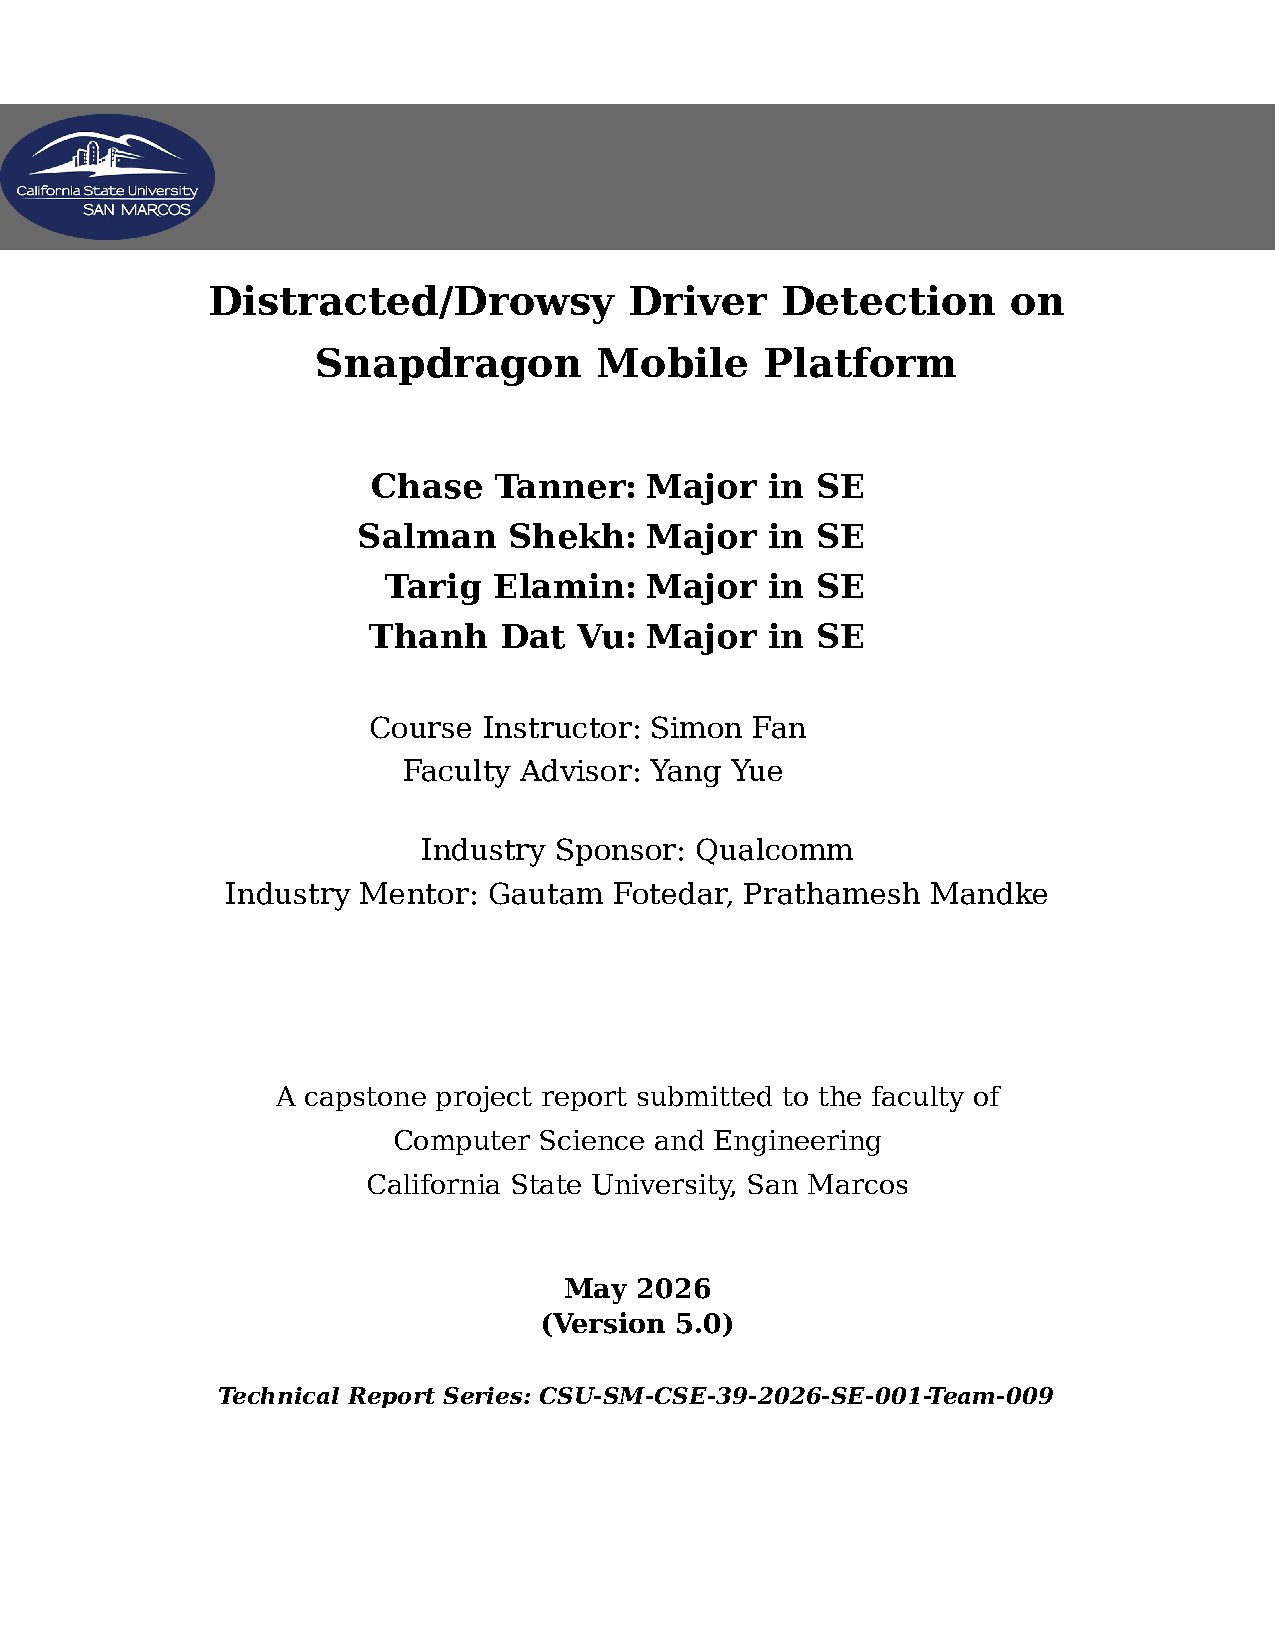
\includepdf[
  pages=1,                       % just the first page of the PDF
  pagecommand={\thispagestyle{empty}}, % ensure no headers/footers/bookmarks on cover
  fitpaper=true,                 % scale to full page
]{assets/CSU-SM-CSE-39-2026-SE-001-Team-009-V5.pdf}

\clearpage

% reset numbering to start after the cover
\pagenumbering{arabic}
\setcounter{page}{1}



% ========================= TOC =========================
\tableofcontents
{\color{qcRed}\rule{16cm}{2pt}}

\clearpage

% ========================= Abstract =========================
\chapter{Abstract}
\textit{ALVION} is an Android application that detects signs of driver drowsiness and distraction using the phone’s front-facing camera and on-device computer vision. Many new vehicles include driver-monitoring features, but millions of older cars do not. Our goal is to help close that gap with a low-cost, widely accessible solution that can run on everyday Android devices and provide timely safety alerts during real driving.
In addition to being a prototype safety application, ALVION serves as a practical testbed to evaluate the real-world capability of Qualcomm-enabled mobile AI for this use case. We focus on whether mobile vision models and on-device acceleration are strong and stable enough to support driver-monitoring signals under realistic conditions (lighting changes, head movement, brief tracking loss, and different mounting angles). These findings help inform what is feasible today on commodity smartphones and what improvements are needed for more robust edge-based driver safety systems.
The system analyzes live video to extract visual cues related to fatigue and inattention, applies configurable thresholds and time-based logic, and triggers clear alerts through sound, on-screen prompts, and vibration when attention appears to drift. While core detection runs on-device for low latency, the application also includes standard product features such as user authentication (e.g., Firebase [3]) to support a realistic app workflow. We do not attempt vehicle integration, cloud-based video processing, large-scale deployment, or regulatory certification.
This document outlines the project’s objectives, assumptions, and boundaries so developers, mentors, and faculty can stay aligned as the system evolves from concept to implementation. It describes the architecture, component responsibilities, and design decisions with an emphasis on building something practical within an academic timeline and extensible for future teams.

% ========================= DOC INFO =========================
\chapter{Report Revision History}

\begin{center}
\begin{tabular}{p{1.8cm} p{2.6cm} p{10.6cm}}
\toprule
\textbf{Version} & \textbf{Date} & \textbf{Description of Changes} \\
\midrule
1.5 & Nov 25, 2025 & Initial draft submitted. Revised structural and behavioral design placeholders per faculty feedback; added preliminary UML comments, ERD rationale, and UI mockups. Corrected terminology in diagrams and aligned architecture descriptions with grading criteria. \\[6pt]
2.0 & Dec 2, 2025  & Completed full capstone design document. Expanded all Requirements; finalized Architecture, Structural, and Behavioral Designs (MVC diagram, class diagrams, ERD, sequence and state diagrams); added UI mockups; completed Exploratory Studies, System Implementation, and System Testing sections. \\[6pt]
2.5 & Dec 11, 2025 & Addressed instructor comments on context/scope diagrams, user--use-case cross-references, non-functional requirement grouping, and algorithm complexity; polished figures and layout. \\[6pt]
3.0 & Feb 28, 2026 & Revised report to reflect updated user requirements and system development changes; confirmed system designs in Section~6; added/updated test case designs and execution reports; incorporated changed/new user requirements into refined system requirements and updated system design. \\[6pt]
3.5 & Mar 20, 2026 & Revised based on instructor feedback. Added Requirements Traceability (Section~4.3) mapping UF-A--UF-J to components and test cases. Introduced Sections~8.4 and~8.5 for functional/non-functional requirement evaluation. Refined scope, use-case alignment, and system consistency. \\[6pt]
4.0 & Apr 27, 2026 & Change-management revision. Corrected detection thresholds (drowsiness 1200\,ms, distraction 4000\,ms/2000\,ms). Added new requirements UF-K, SF-11--SF-15. Updated architecture, ERD, UI, and algorithm sections to document TFLite sunglasses detection, Firestore trip history, GPS speed, phone orientation monitoring, and presence check. Fixed structural gaps to conform to capstone report guidelines. \\[6pt]
5.0 & May 11, 2026 & Final revision for capstone submission. Completed proofreading and language polish across all sections. Verified all chapters are present and consistently structured. Confirmed all eleven user functional requirements (UF-A through UF-K) are implemented and documented. No structural changes; this version represents the final submitted state of the report. \\
\bottomrule
\end{tabular}
\end{center}

\clearpage

% ========================= 3. PROBLEM & CONTEXT =========================
\chapter{Problem Statement}


\section{Business Background}
Driver monitoring is becoming a regulatory and industry standard for road safety. The European Union now mandates such systems in new vehicles beginning in 2024 [6], and other markets are expected to follow. Automakers and regulators view these systems as essential for reducing human-error-related crashes, but adoption in existing vehicles remains limited because of cost, integration complexity, and consumer concerns over data privacy.
Retrofit products, while available, often require expensive hardware installations or continuous cloud connectivity for processing. These barriers restrict adoption, especially in regions where consumers rely on older cars or are reluctant to share biometric data online. A smartphone-based solution reduces those barriers: most users already own compatible Android devices with capable cameras and neural-processing hardware.
ALVION’s approach uses these resources to demonstrate how Qualcomm’s mobile AI platforms can perform effective, real-time driver-monitoring inference entirely on-device. This provides a testbed for cost-effective safety innovations and shows potential business alignment with regulatory trends. The project also establishes a baseline for future Qualcomm-enabled automotive safety research and gives developers a model for edge-based AI deployment that respects user privacy and reduces infrastructure costs.

\clearpage

\section{Needs}
Improving driver safety requires early detection of distraction and drowsiness in a manner that is both reliable and user-friendly. ALVION responds to several intertwined needs:

\begin{itemize}
    \item \textbf{Safety:} The system should protect both the driver and other road users by recognizing behavioral cues such as prolonged eyelid closure, yawning, or abnormal head pose patterns that precede dangerous inattention. Distraction-affected crashes alone caused 3{,}208 U.S. fatalities in 2024 [7].
    \item \textbf{Privacy-Aware Design:} Drivers are wary of surveillance systems that upload facial video to the cloud. ALVION is designed to keep \emph{core detection and inference on-device} and avoid transmitting raw camera footage, while still supporting standard app functionality such as user authentication (e.g., Firebase [3]).
    \item \textbf{Accessibility and Cost:} Full-scale automotive integrations are expensive. By leveraging common smartphone hardware, ALVION provides a low-cost entry point that can benefit drivers in older vehicles.
    \item \textbf{Responsiveness:} Alerts must reach the driver when they matter most. Real-time analysis enables immediate feedback that can help prevent incidents instead of only documenting them.
    \item \textbf{Reusability and Scalability:} The project serves as a reference implementation that can be adapted, expanded, and optimized by future teams, supporting continuous improvement in mobile AI safety systems and evaluation of mobile AI model capability.
\end{itemize}
\clearpage

\section{Objectives}
ALVION’s objectives focus on producing a working, reproducible prototype that demonstrates the technical and practical viability of phone-based driver monitoring:

\begin{itemize}
  \item \textbf{Develop a proof-of-concept Android application} capable of detecting drowsiness and distraction using the front camera and a lightweight on-device model optimized for Snapdragon NPUs [13].
  \item \textbf{Implement configurable alert mechanisms} that combine audio, visual, and haptic feedback, allowing users to tune thresholds and notification styles for comfort and responsiveness.
  \item \textbf{Achieve efficient real-time performance} without dependence on cloud computing, ensuring low latency and minimal power usage consistent with mobile operation.
  \item \textbf{Document all design decisions, architecture, and testing methodology} in a reproducible form so that future development teams can extend or refine the system.
  \item \textbf{Conduct iterative testing and evaluation} under varying lighting, motion, and device conditions to measure accuracy, usability, and overall system robustness.
\end{itemize}

Through these objectives, ALVION demonstrates a concrete pathway from concept to functional prototype, aligning technical feasibility with ethical design and industry safety goals.
\clearpage


% ========================= 4. USER REQUIREMENTS =========================
\chapter{Requirements}
\section{User Requirement}
\subsection{Glossary of Relevant Domain Terminology}

\begin{description}

    \item[ALVION] The Android-based driver drowsiness and distraction detection mobile application developed for this capstone project. Runs entirely on-device to ensure privacy and real-time performance.

    \item[Driver Monitoring System (DMS)] A safety technology that uses sensors or cameras to assess driver attention, alertness, and potential fatigue while operating a vehicle.

    \item[Head Yaw] The horizontal rotation of a driver’s head relative to the camera. Excessive yaw over time indicates potential distraction or inattention.

    \item[Yaw Delta] The angular difference between the driver's current head yaw and their calibrated forward baseline.

    \item[Android Studio] The official integrated development environment (IDE) for Android applications. Used to develop and build the ALVION mobile app using Kotlin.

    \item[Kotlin] A modern programming language fully supported by Android, known for concise syntax and null safety. Used as the primary implementation language for ALVION.

    \item[Jetpack Compose] Android’s declarative UI framework written in Kotlin. It simplifies the creation of reactive, adaptive user interfaces without the need for XML layout files.

    \item[CameraX [2]] A Jetpack library that provides easy access to camera functions such as preview, capture, and frame analysis. Used in ALVION to stream frames for real-time inference.

    \item[ML Kit Face Detection [1]] Google’s on-device machine learning SDK used in ALVION to provide real-time eye-openness probabilities and head pose (Euler angles) without requiring a custom-trained model.

    \item[Firebase Authentication [3]] A cloud-based service used to manage user identity and secure login flows within the application.

    \item[Calibration Buckets] Specific data collections (e.g., "forward", "left", "right") used during the setup phase to establish baseline eye-openness and head-pose values for an individual driver.

    \item[Mirror Symmetry Logic] A heuristic used during calibration to infer eye-closure thresholds for one side of the face based on the other, improving system robustness when a driver only calibrates one side mirror.

    \item[Exponential Moving Average (EMA)] A statistical smoothing technique applied to eye-openness scores to reduce noise and prevent flickering alerts caused by momentary blinks or sensor jitters.

    \item[Debounce / Alert Cooldown] Software mechanisms that prevent repeated, rapid-fire triggers of an alert within a short time window, ensuring that warnings remain helpful rather than distracting.

    \item[Latency] The time delay between camera frame capture and alert output. Low latency is critical to ensure timely driver warnings.

    \item[FPS (Frames Per Second)] A measure of how many frames are processed per second during video analysis. Maintaining $\geq$15 FPS ensures smooth real-time inference.

    \item[On-device Inference] The process of running AI models locally on the phone rather than sending data to cloud servers. Essential for preserving privacy and minimizing delay.

    \item[Privacy by Design] A principle ensuring that user data (especially facial video) remains on the device and is not transmitted externally without explicit consent.

\end{description}

\subsection{User Groups}
This section describes the primary user groups who interact with ALVION today, as well as optional stakeholders shown in the context/scope diagrams as potential future extensions.

\begin{itemize}
    \item \textbf{End Users (Drivers):} Primary users who run the app during driving and rely on real-time alerts and feedback to help detect potential drowsiness or distraction.
    \item \textbf{Developers / Maintainers:} Internal users responsible for building, testing, maintaining, and improving the system (e.g., updating detection logic, calibration flow, app UX, and configuration).
    \item \textbf{Optional / Future Stakeholders:} Roles such as fleet managers or system administrators may be supported in later iterations (e.g., aggregated summaries or managed configuration), but are not part of the current MVP.
\end{itemize}

\subsection{Project Context}
\begin{figure}[H]
    \centering
    \includegraphics[width=0.95\textwidth]{assets/context_diagram_v1.png}
    \caption{System context diagram for the ALVION driver drowsiness and distraction detection mobile application}
    \label{fig:context}
\end{figure}

\noindent
The context diagram illustrates how the ALVION mobile application interacts with its surrounding environment.
The driver provides a live camera feed through the smartphone’s front-facing camera and receives real-time alerts through audio, vibration, and visual cues.
The application communicates with the Android OS using standard APIs for camera access [2], permissions, audio output, vibration, and local storage.
Core detection is performed on-device using a mobile face-detection pipeline (e.g., ML Kit [1]) to estimate signals such as eye openness and head pose for time-based alerting.
The system may also integrate cloud-backed application features such as authentication (e.g., Firebase [3]) to support a realistic app workflow.
Optional connections shown in the diagram (e.g., aggregated summaries or managed configuration) represent potential future extensions rather than required MVP functionality.

\subsection{Functional Requirements}
\subsubsection{Project Scope}
\begin{figure}[H]
\centering
\includegraphics[width=0.95\textwidth]{assets/project_scope_v1.jpg}
\caption{Scope diagram to illustrate major user interactions with ALVION}
\label{fig:scope}
\end{figure}

\subsubsection{User Scenarios}
The following scenarios describe how end users interact with the ALVION mobile application during setup, monitoring, and post-session review. Each scenario corresponds to a use case identified in the Project Scope diagram and summarized in Appendix~U.
\begin{itemize}

    \item \textbf{Start Monitoring Session:}
    The driver launches ALVION, completes sign-in if required, grants camera permissions, and starts a monitoring session. The app activates the front-facing camera through CameraX and initializes the face-detection pipeline to estimate eye openness and head pose in real time.

    \item \textbf{Receive Drowsiness Alert:}
    During monitoring, ALVION evaluates eye-closure behavior over time. If eye closure persists beyond a configured duration threshold, the system issues an audible and on-screen alert (and optional vibration) to prompt the driver to refocus or take a break.

    \item \textbf{Receive Distraction Alert:}
    ALVION monitors head orientation relative to the calibrated forward baseline. If the driver’s head remains turned away from the forward direction beyond the configured threshold window, the system triggers a distraction alert.

    \item \textbf{Acknowledge or Mute Alerts:}
    After an alert is issued, the driver can acknowledge it and, if needed, temporarily mute alerts. The system applies a cooldown interval to prevent repeated notifications in rapid succession.

    \item \textbf{Adjust Settings in Profile Tab:}
    The driver opens the Profile/Settings screen to update preferences (e.g., alert enablement, sensitivity thresholds, vibration/sound options, and emergency contact settings). Settings persist between sessions and may be stored securely (e.g., via Firebase) depending on the current implementation.

    \item \textbf{Calibrate / Align Camera:}
    On first use, after device repositioning, or when calibration quality degrades, the driver completes a short calibration flow to align the camera and establish a baseline. The app provides live feedback to guide the driver until calibration succeeds.

    \item \textbf{Emergency Contact / Call for Help:}
    If the driver believes they are unsafe to continue (e.g., repeated drowsiness warnings), the driver can use an emergency action to place a call to \textbf{911} or a designated family member/emergency contact. This action is intentionally user-initiated to avoid accidental calls.

    \item \textbf{View Trip History:}
    After ending a session, the driver can navigate to the \textbf{History} tab to review past trips. Each trip card displays the date, duration, start time, and a categorized list of safety detections (drowsiness, distraction, presence check, phone orientation). Trip records are automatically saved to Firebase Firestore and persist across app restarts.

    \item \textbf{Live Speed and Duration Metrics:}
    While a session is active, the app displays real-time trip duration and current GPS speed (km/h) in a metrics grid below the camera view. GPS speed is obtained via the Android Fused Location Provider and requires location permission.

    \item \textbf{Phone Orientation Warning:}
    If the phone is detected as physically upside-down during monitoring (using the accelerometer and display rotation API), the system immediately issues an alert prompting the driver to flip the device. This detection is debounced to avoid false triggers from sensor noise.

\end{itemize}

\subsubsection{User Functional Requirements}
This section provides short descriptions of the user functional requirements identified for the ALVION mobile application. Each requirement defines a specific capability the system provides to meet the goals of the drivers and the technical needs of the development team.

\begin{enumerate}

    \item \textbf{UF-A: Account Management} —
    The system shall allow drivers to create an account and securely log in using Firebase Authentication [3] to manage personal session history and preferences.

    \item \textbf{UF-B: Drowsiness Detection and Alerting} —
    The system shall continuously analyze eye openness using the PERCLOS metric [4] and issue a warning when sustained eyelid closure (exceeding a defined millisecond threshold) indicates drowsiness. (Supported by Use Cases UC-001 and UC-002.)

    \item \textbf{UF-C: Distraction Detection and Alerting} —
    The system shall detect when the driver’s head yaw deviates from the calibrated forward baseline for longer than a defined interval and trigger an attention-restoring alert. (Supported by Use Case UC-010.)

    \item \textbf{UF-D: Configurable Sensitivity and Alert Settings} —
    The system shall provide a settings interface that allows the driver to adjust detection sensitivity, alert volume, and the "cooldown" period between consecutive alerts. (Supported by Use Case UC-004.)

    \item \textbf{UF-E: Start and Stop Monitoring Session} —
    The driver shall be able to manually start and end a monitoring session, which handles the lifecycle of the CameraX stream [2] and the ML Kit inference pipeline [1]. (Supported by Use Case UC-001.)

    \item \textbf{UF-F: Real-Time Alert Delivery} —
    The system shall deliver immediate visual, audio, and haptic (vibration) feedback when drowsiness or distraction is detected to ensure driver response. (Supported by Use Cases UC-002 and UC-010.)

    \item \textbf{UF-G: Acknowledge or Snooze Alerts} —
    The system shall allow the driver to acknowledge an active alert or temporarily snooze notifications during short recovery periods. (Supported by Use Case UC-003.)

    \item \textbf{UF-H: Multi-Stage Camera Calibration} —
    The system shall provide a calibration routine to establish the driver's forward-facing baseline. This includes "Mirror Logic" to infer eye-closure thresholds for side-mirrors based on partial calibration data. (Supported by Use Case UC-005.)

    \item \textbf{UF-I: Trip History and Session Persistence} —
    The system shall automatically save each completed monitoring session as a \texttt{Trip} record in Firebase Firestore, including start/end timestamps, duration, and a timestamped list of alert events (drowsiness, distraction, presence check, phone orientation). The driver shall be able to view all past trips in a dedicated \textbf{History} tab and clear the history if desired. (Supported by Use Cases UC-006 and UC-007.)

    \item \textbf{UF-J: Privacy and Local Data Control} —
    The system shall process all camera frames locally. No raw video or identifiable facial images shall be transmitted externally; only anonymized alert metadata (event type, timestamp) may be stored in the cloud via Firestore. (Emphasized in Use Cases UC-001 and UC-006.)

    \item \textbf{UF-K: Sunglasses and Occlusion Detection} —
    The system shall use a custom TFLite binary classifier to detect when the driver is wearing sunglasses during a monitoring session. When sunglasses are detected, the drowsiness detection pipeline shall be suppressed and the driver shall be notified that eye-based monitoring is paused, while head-pose distraction monitoring continues unaffected.

\end{enumerate}

% ---------- 4.1.5 User Non-functional Requirements ----------
\subsection{Non-functional Requirements}
The following non-functional requirements capture quality and constraint expectations from the driver's perspective. Full descriptions are provided in Appendix~R.

\subsubsection{Product: Usability Requirements}
The driver must be able to start a monitoring session in under two taps. Alerts must be clear, well-timed, and non-distracting.

\subsubsection{Product: Performance Requirements}
The system must respond in real time ($\leq$200\,ms alert latency) and maintain smooth frame analysis without perceptible lag.

\subsubsection{Product: Availability/Reliability/Security}
Core monitoring must remain stable for a full driving session ($\geq$60 minutes). User credentials must be securely managed and not exposed.

\subsubsection{Organizational: Development Requirements}
The system shall be built on standard Android tools (Kotlin, Jetpack Compose) to ensure maintainability by future development teams.

\subsubsection{Organizational: Operational Requirements}
Core detection must function without an active internet connection. GPS and history features may require connectivity.

\subsubsection{Organizational: Environmental Requirements}
The app must operate reliably under varied in-car lighting (day, night, overcast) and across different mounting angles.

\subsubsection{External: Legislative Requirements on Safety/Security}
The system shall comply with mobile privacy best practices by keeping facial data on-device and not storing biometric identifiers.

\subsubsection{External: Cultural and Social Requirements}
The system should function equitably across drivers of diverse skin tones and facial structures as supported by ML Kit.

\subsubsection{External: Interoperability Requirements}
The application targets Android SDK 24 minimum, ensuring broad device compatibility without requiring proprietary hardware.

% ========================= 4. SYSTEM REQUIREMENTS =========================
\section{\textcolor{qcRed}{System Requirements}}

% ---------------- 4.2.1 Functional Requirements ----------------
\subsection{Functional Requirements}

% 4.2.1.1 System Functional Requirements
\subsubsection{System Functional Requirements}
The ALVION system shall implement the following core functional features to enable real-time driver monitoring and alerting:

\begin{itemize}
    \item \textbf{SF-01: Real-Time Drowsiness Detection} —
    The system shall utilize the ML Kit Face Detection API [1] to analyze eye-openness probabilities. Using the PERCLOS metric [4], it shall trigger an alert when the EMA-smoothed eye score remains below the calibrated threshold for more than $1{,}200$\,ms (default drowsiness trigger duration).

    \item \textbf{SF-02: Distraction Detection} —
    The system shall track head yaw (horizontal rotation) and issue a distraction alert using a tiered dwell-time hierarchy: $4{,}000$\,ms when the driver's head is within a calibrated mirror-check range, and $2{,}000$\,ms when the deviation exceeds that range (e.g., looking at a phone or passenger).

    \item \textbf{SF-03: Multi-Stage Alert Mechanisms} —
    The system shall deliver synchronous alerts using audio tones, haptic vibration, and visual UI overlays to ensure the driver is promptly notified of safety risks.

    \item \textbf{SF-04: Account and History Management} —
    The system shall provide a secure login interface via Firebase Authentication [3], allowing drivers to maintain personal session statistics and persistent device configurations.

    \item \textbf{SF-05: Dynamic Calibration and Mirror Logic} —
    The system shall establish a forward-facing baseline during setup. It shall include "Mirror Symmetry" logic to automatically infer detection thresholds for side-viewing angles based on partial user calibration.

    \item \textbf{SF-06: Configurable Thresholds} —
    The system shall allow the driver to adjust eye-closure sensitivity, head-pose thresholds, and the "alert cooldown" period via a dedicated Settings interface.

    \item \textbf{SF-07: Session Control and Lifecycle} —
    The application shall allow users to manually start and stop monitoring, correctly managing the Android CameraX lifecycle [2] and ML inference pipeline [1].

    \item \textbf{SF-08: Snooze and Acknowledge Logic} —
    The system shall provide interactive UI elements to acknowledge or temporarily snooze active alerts, preventing repetitive notifications once the driver has regained focus.

    \item \textbf{SF-09: Local Privacy and Data Protection} —
    All frame analysis shall occur strictly on-device. The system shall store session summaries and event logs in secure, app-scoped storage, with no transmission of raw video data to external servers.

    \item \textbf{SF-10: Session Summary Reporting} —
    Upon ending a session, the app shall generate a report summarizing the frequency and type of alerts triggered and persist this record to Firebase Firestore for the authenticated user.

    \item \textbf{SF-11: Real-Time GPS Speed Display} —
    During an active monitoring session, the system shall display the driver's current speed in km/h using the Android Fused Location Provider. Location updates shall be polled at 1-second intervals and the display shall revert to 0 km/h when the session ends or location permission is unavailable.

    \item \textbf{SF-12: Phone Orientation Monitoring} —
    The system shall detect when the device is physically upside-down during a session using the accelerometer sensor and display rotation API. Upon confirming an inverted orientation (debounced by 250\,ms), it shall issue a warning alert and log a \texttt{PHONE\_UPSIDE\_DOWN} event to the current session record.

    \item \textbf{SF-13: TFLite Sunglasses Detection} —
    The system shall run a custom binary TFLite classifier (\texttt{sunglasses\_model.tflite}) on a cropped face region every 3 frames during monitoring. When sunglasses are detected with confidence $\geq 0.70$ for 2 consecutive inferences, drowsiness detection shall be suppressed and the eye-occlusion state shall be set. Detection shall be cleared when confidence falls below $0.45$ for 2 consecutive inferences.

    \item \textbf{SF-14: Presence / Liveness Check} —
    When eye landmarks are occluded and the detected face position and head rotation remain statistically static for $10{,}000$\,ms (variance below defined thresholds), the system shall issue a presence-check alert prompting the driver to confirm alertness by moving their head.

    \item \textbf{SF-15: Face Proximity Guard} —
    The system shall detect when the driver's face occupies more than 60\% of the camera frame area (indicating the device is too close to the face) and temporarily suspend safety monitoring for that frame, preventing unreliable landmark readings from triggering false alerts.
\end{itemize}

% ---------------- 4.2.1.2 Data Requirements ----------------
\subsubsection{Data Requirements}
The ALVION application manages data related to user identity, real-time facial analysis, and session-specific calibration. Since the system utilizes a pre-trained ML Kit model, data handling is focused on user authentication and the transient processing of camera frames.

\paragraph{Data Inputs}
\begin{itemize}
    \item \textbf{User Authentication Data:} Email and password credentials provided during login/signup, managed via Firebase Authentication [3].
    \item \textbf{Live Camera Feed:} RGB frames captured via CameraX [2], used exclusively for real-time inference and never stored.
    \item \textbf{Facial Landmark Metrics:} Raw probability scores (eye-openness) and Euler angles (head rotation) provided by the ML Kit Face Detection API [1].
\end{itemize}

\paragraph{Data Processing and Storage}
\begin{itemize}
    \item \textbf{User Profiles (Cloud):} Basic user identity data is stored securely in Firebase Authentication to manage accounts across sessions.
    \item \textbf{Trip History (Cloud):} Each completed monitoring session is saved as a \texttt{Trip} document in Firebase Firestore (\texttt{trips} collection), containing the user ID, date label, start/end timestamps, duration, and a list of \texttt{TripAlert} events (type and timestamp). This data is scoped per authenticated user and persists indefinitely until the driver clears it.
    \item \textbf{Calibration Baselines (Local):} Yaw offsets and eye-closure thresholds are calculated during calibration and stored locally in SharedPreferences to maintain the user's forward baseline for the duration of the app's use.
    \item \textbf{Session Metrics (Volatile):} Running EMA scores for eye openness and head-pose state are maintained in-memory and discarded once the monitoring session ends. Raw video frames are never written to storage.
\end{itemize}

\paragraph{Data Quality and Privacy}
\begin{itemize}
    \item \textbf{On-Device Processing:} All facial analysis is performed locally. No raw images, video, or biometric "face-print" data is transmitted to Firebase or any external server.
    \item \textbf{Threshold Clamping:} Eye-openness values are strictly clamped between 0 and 1 to ensure consistent alert triggers across different lighting conditions.
    \item \textbf{Secure Authentication:} Password management and token handling are delegated to Firebase, ensuring industry-standard security for user accounts.
\end{itemize}

\textit{While user identity and anonymized alert metadata are managed in the cloud, all privacy-sensitive facial data remains volatile and local to the driver's device.}

% ---------- 4.2.2 Non-functional Requirements ----------
\subsection{Non-functional Requirements}
This section defines the technical constraints and quality standards the ALVION system must meet. These requirements serve as the benchmarks for system testing and performance evaluation.

\subsubsection{Product: Usability Requirements}
\begin{itemize}
    \item \textbf{SP-01-01} — The interface shall allow a driver to initiate monitoring in under two taps to ensure minimal distraction during vehicle setup.
    \item \textbf{SP-02-01} — The system shall maintain hands-free operation; no manual input shall be required or accepted while a monitoring session is active.
    \item \textbf{SP-04-01} — The application shall display a safety disclaimer upon launch that must be acknowledged before the driver can access monitoring features.
\end{itemize}

\subsubsection{Product: Performance Requirements}
\begin{itemize}
    \item \textbf{SP-05-01} — The inference pipeline shall maintain a minimum of 15 FPS and an alert latency of $\leq$200\,ms on supported Snapdragon devices.
    \item \textbf{SP-05-02} — Average CPU utilization shall remain below 40\% by utilizing the Android Neural Networks API (NNAPI) [12] for ML Kit hardware acceleration.
    \item \textbf{SP-07-01} — The system shall include thermal management logic that reduces inference frequency if the device temperature exceeds safe operating limits.
\end{itemize}

\subsubsection{Product: Availability, Reliability, and Security}
\begin{itemize}
    \item \textbf{SP-03-01} — Visual, auditory, and haptic alerts shall be synchronized within $\pm$50\,ms to provide a clear, unified warning to the driver.
    \item \textbf{SP-08-01} — The application shall remain operational for at least 60 minutes of continuous monitoring without crash or significant performance degradation.
    \item \textbf{SP-09-01} — In the event of a camera obstruction or ML failure, the system shall provide a "Tracking Lost" notification within 3 seconds of continuous landmark loss.
    \item \textbf{SP-10-01} — All facial analysis shall be performed locally. No raw images or video data shall be transmitted externally or stored permanently.
\end{itemize}

\subsubsection{Organizational: Development Requirements}
\begin{itemize}
    \item \textbf{SO-01-01} — The project shall be implemented using Kotlin and Jetpack Compose, targeting Android SDK 33 (Android 13) or higher.
\end{itemize}

\subsubsection{Organizational: Operational Requirements}
\begin{itemize}
    \item \textbf{SO-09-01} — Core detection and alerting features must function without an active internet connection (strictly offline monitoring).
\end{itemize}

\subsubsection{Organizational: Environmental Requirements}
\begin{itemize}
    \item The system shall operate across typical automotive lighting environments, including low-light night driving and high-glare daytime conditions.
\end{itemize}

\subsubsection{External: Legislative Requirements on Safety/Security}
\begin{itemize}
    \item \textbf{SE-01-01} — The application shall comply with mobile safety standards by disabling configuration menus while the vehicle is detected to be in motion.
\end{itemize}

\subsubsection{External: Cultural and Social Requirements}
\begin{itemize}
    \item \textbf{SE-03-01} — The system shall be validated for consistent landmark detection across varied skin tones and common eyewear (glasses).
\end{itemize}

\subsubsection{External: Interoperability Requirements}
\begin{itemize}
    \item The system shall integrate with Firebase Authentication and Firestore using standard Google Play Services APIs, without dependency on proprietary device-specific SDKs.
\end{itemize}

% ---------- 4.3 Requirements Trace Table ----------
\section{Requirements Trace Table}

A Requirements Traceability Table is provided in Appendix R to ensure that all user requirements are systematically mapped to system functionality, design components, and testing procedures.

This table establishes clear relationships between:
\begin{itemize}
    \item User Functional Requirements (UF-A through UF-K)
    \item System Functional Requirements (SF-01 through SF-15)
    \item Design components such as the \texttt{FaceDetectionAnalyzer}, \texttt{FaceStateEvaluator}, \texttt{SunglassesClassifier}, \texttt{HistoryRepository}, and \texttt{SpeedTracker}
    \item Corresponding test cases used for validation
\end{itemize}

This traceability ensures that every requirement is:
\begin{itemize}
    \item Properly implemented within the system
    \item Verified through testing
    \item Consistent with the overall system architecture
\end{itemize}

By maintaining this mapping, the project guarantees completeness, reduces the risk of missing functionality, and improves maintainability for future development.

% ========================= 5. EXPLORATORY STUDIES =========================
\chapter{Exploratory Studies}\label{ch:exploratory-studies}

% ---------- 5.1 Relevant Development Frameworks ----------
\section{Relevant Development Frameworks}\label{sec:frameworks}
We are building a phone-first prototype that runs entirely on the device. To ensure real-time performance and reliability on Android, we have selected a modern, native stack that minimizes external dependencies.

\subsection{Android Studio (Kotlin)}
\textbf{What it is.} Android Studio is the official IDE; \textbf{Kotlin} is the primary implementation language.
\textbf{Why we use it.} It provides the most robust support for modern Android development, including built-in profiling tools to monitor CPU and thermal impact during long driving sessions.

\subsection{Front end: Jetpack Compose (Material3)}
\textbf{What it is.} Compose is Android’s modern declarative UI toolkit [8].
\textbf{Why we use it.} It allows us to build responsive, high-performance UI overlays (e.g., the camera preview and alert badges) that react instantly to changes in the driver's attention state without the overhead of XML-based layouts.

\subsection{Camera: CameraX (Preview + Analysis)}
\textbf{What it is.} A Jetpack library [2] that simplifies camera integration.
\textbf{Why we use it.} CameraX allows us to split the camera feed into two paths: a low-latency preview for the user and a continuous "Analysis" stream of image proxies. It handles device rotation and lifecycle management automatically, ensuring the app doesn't crash when backgrounded.

\subsection{Inference: ML Kit Face Detection}
\textbf{What it is.} An on-device Qualcomm SDK [1] for vision tasks.
\textbf{Why we use it.} ML Kit provides a pre-trained, highly optimized pipeline for facial landmarking. It returns the exact metrics needed for our safety logic—specifically eye-openness probabilities and head Euler angles (yaw)—without the need for custom model training or hosting.

\subsection{Backend: Firebase Authentication and Firestore}
\textbf{What it is.} A secure cloud-based identity and database platform [3].
\textbf{Why we use it.} Firebase Authentication handles secure login and account management. Firebase Firestore stores each completed trip as a structured document (alert types, timestamps, duration) scoped to the authenticated user, enabling persistent trip history across sessions without transmitting any raw facial data.

\subsection{On-Device Custom Classifier: TFLite}
\textbf{What it is.} The TensorFlow Lite runtime for Android (now distributed as LiteRT) [10].
\textbf{Why we use it.} ML Kit does not provide a sunglasses-detection signal. We trained and deployed a custom binary TFLite model (\texttt{sunglasses\_model.tflite}) that classifies $128 \times 128$ cropped face images as sunglasses / no-sunglasses. Running this classifier every 3 frames suppresses false drowsiness detections caused by eye occlusion from dark lenses.

\subsection{Location: Fused Location Provider}
\textbf{What it is.} Google Play Services' battery-efficient location API.
\textbf{Why we use it.} We use the Fused Location Provider [11] to stream GPS speed updates at 1-second intervals during active sessions, displayed in the live metrics grid. This context (speed = 0 vs. highway speed) helps drivers understand their monitoring state.

\subsection{Project Glue: Coroutines and Flow}
\textbf{What it is.} Kotlin’s asynchronous programming primitives.
\textbf{Why we use it.} We use \textbf{Coroutines} [9] to keep the heavy ML analysis off the main UI thread. \textbf{Flow} allows us to stream detection events (e.g., a "Drowsy" signal) from the logic layer to the UI layer in real-time with minimal latency.

\subsection*{Tool roles at a glance}
\begin{center}
    \begin{tabular}{p{4.0cm} p{5.0cm} p{6.4cm}}
        \toprule
        \textbf{Tool} & \textbf{Role} & \textbf{Why it’s in the stack} \\
        \midrule
        Android Studio + Kotlin & App development & Native toolchain; full hardware access.\\
        \\
        Jetpack Compose & Declarative UI & Reactive alerts and polished components.\\
        \\
        CameraX & Frame Analysis & Reliable frame capture; handles rotation.\\
        \\
        ML Kit Face Detection & Vision Inference & Pre-trained metrics for eyes and yaw.\\
        \\
        TFLite Interpreter & Sunglasses Detection & Custom binary classifier for eye occlusion.\\
        \\
        Firebase Auth + Firestore & User Accounts + History & Login and persistent trip records.\\
        \\
        Fused Location Provider & GPS Speed & Real-time speed display during sessions.\\
        \\
        Kotlin Coroutines & Concurrency & Keeps UI responsive during ML tasks.\\
        \bottomrule
    \end{tabular}
\end{center}

% ---------- 5.2 Relevant Solution Techniques ----------
\section{Relevant Solution Techniques}\label{sec:solutions}
ALVION utilizes a heuristic-based detection engine built on top of pre-trained facial landmark metrics provided by ML Kit. Rather than training a custom classifier, our technique focuses on \textbf{subject-specific calibration} and \textbf{temporal smoothing} to ensure accuracy across different drivers and mounting angles.

\subsection{Calibration Strategy: Multi-Angle Scan}
A core innovation of the system is the multi-angle calibration routine, which establishes the driver's unique visual geometry before monitoring begins. This prevents false alerts caused by natural variations in seating position or device mounting.

\begin{itemize}
    \item \textbf{Forward Baseline Establishment:} The driver is prompted to look straight ahead at the road. The system captures a series of frames to establish a \texttt{forwardYawBaseline}. All subsequent head movements are calculated as a \textit{Yaw Delta} relative to this baseline.
    \item \textbf{Mirror Angle Bucketing:} The system provides specific "buckets" for the Left Mirror, Center/Forward, and Right Mirror. During calibration, the driver scans these positions, and the system records the specific Euler Y (yaw) angles and eye-openness ranges for each.
    \item \textbf{Mirror Symmetry Logic:} To minimize setup time, the system implements symmetry-based inference. If a driver only calibrates the "Left Mirror" bucket, the system automatically calculates the expected "Right Mirror" yaw and eye-thresholds by mirroring the left-side data relative to the forward baseline.
\end{itemize}

\subsection{Detection Logic: Eye Thresholds and Head Pose}
The detection engine processes the calibrated data using two parallel logic paths for Drowsiness and Distraction.

\paragraph{Drowsiness (Sustained Eye Closure):}
The system implements a \textbf{PERCLOS Proxy [4, 5]} (Percentage of Eyelid Closure) using a duration-based trigger.
\begin{enumerate}
    \item \textbf{EMA Smoothing:} Raw eye-openness scores from ML Kit are processed using an \textit{Exponential Moving Average} [14] ($\alpha = 0.45$) to filter out momentary blinks and sensor noise.
    \item \textbf{Dynamic Thresholding:} Instead of a fixed 0.5 threshold, the system uses the eye-openness stats gathered during calibration to set a custom "closed" threshold for each driver.
    \item \textbf{Temporal Trigger:} If the EMA eye-score remains below the threshold for more than $1{,}200$~ms, a "Drowsy" event is published to the alert manager.
\end{enumerate}

\paragraph{Distraction (Yaw Deviation):}
Distraction is detected by monitoring the \textit{Yaw Delta} against a dwell-time hierarchy.
\begin{enumerate}
    \item \textbf{Mirror-Check Tolerance:} If the driver is looking toward a calibrated mirror angle, the system allows a dwell time of $4{,}000$~ms to account for normal traffic checks.
    \item \textbf{Beyond-Mirror Deviation:} If the yaw delta exceeds the mirror range (indicating the driver is looking at a passenger or a phone), a shorter dwell time of $2{,}000$~ms is enforced before an alert is triggered.
    \item \textbf{Yaw Hysteresis:} To prevent alert "flickering" near the threshold, the system requires the head to return $8^\circ$ back toward the center before the distraction state is reset.
\end{enumerate}

\subsection{Evaluation and Tuning Strategy}
Since the system uses a pre-trained model for landmarks, our evaluation focus shifts from "Model Accuracy" to "Pipeline Robustness."

\begin{itemize}
    \item \textbf{Environmental Validation:} The pipeline is tested across three primary lighting conditions: High Noon (direct sunlight), Overcast (diffuse light), and Night (artificial cabin light).
    \item \textbf{Occlusion Testing:} Evaluation specifically targets how well the ML Kit landmarks maintain stability when the driver wears prescription glasses or sunglasses.
    \item \textbf{Latency Benchmarking:} We measure the "End-to-End" latency—from the moment the eyes close to the moment the haptic motor vibrates—to ensure we stay below the $200$~ms performance requirement.
\end{itemize}

\subsection{What ``Success'' Looks Like}
A successful implementation on the Snapdragon target device is defined by:
\begin{itemize}
    \item \textbf{Zero-Cloud Dependency:} All calibration and detection logic executes locally via the ML Kit SDK.
    \item \textbf{Stable 24--30 FPS:} Smooth camera preview and concurrent analysis without thermal throttling.
    \item \textbf{Low False-Positive Rate:} The "Mirror Symmetry" and "EMA Smoothing" logic correctly distinguishes between a long blink and true drowsiness.
\end{itemize}

% ---------- 5.3 Broader Impacts ----------
\section{Broader Impacts}\label{sec:impacts}

The ALVION project demonstrates the feasibility of bringing advanced safety features to a wider demographic without the need for high-cost, integrated vehicle hardware. By leveraging commodity smartphone sensors and on-device ML, the project creates meaningful impacts in road safety and mobile AI application design.

\subsection*{Impact on Individuals (Drivers)}
\begin{itemize}
    \item \textbf{Safety for Legacy Vehicles.} The most immediate impact is on drivers of older vehicles that lack built-in Driver Monitoring Systems (DMS). ALVION provides these users with a low-cost alternative to expensive retrofit hardware, offering real-time alerts that can prevent accidents caused by fatigue or distraction.
    \item \textbf{Empowerment through Awareness.} Because the system provides immediate feedback and a personal "Trip History," it encourages drivers to recognize their own fatigue patterns. This empowers individuals to make informed decisions about when to take breaks, fostering long-term safer driving habits.
    \item \textbf{Low-Barrier Awareness.} Because the system requires only a standard Android device, it encourages safer driving habits through immediate feedback, helping drivers recognize their own fatigue patterns before they become a critical danger.
\end{itemize}

\subsection*{Impact on Organizations}
\begin{itemize}
    \item \textbf{Scalable Fleet Safety.} For organizations such as delivery services or ride-sharing platforms, ALVION offers a software-defined safety solution that can be deployed across a fleet without hardware installation costs. This allows organizations to improve safety standards and reduce liability with minimal capital expenditure.
    \item \textbf{Technical Template for Developers.} The project serves as a proof-of-concept for running complex, real-time vision pipelines (ML Kit and CameraX) on Snapdragon hardware. It provides a template for organizations looking to build responsive, safety-critical applications that must operate reliably at the "edge" without constant cloud connectivity.
    \item \textbf{Resource-Efficient Safety.} The project proves that sophisticated safety signals—like yaw delta and eyelid closure—can be computed with minimal battery and thermal impact, setting a baseline for what is achievable in modern edge-based AI.
\end{itemize}

\subsection*{Impact on Society}
\begin{itemize}
    \item \textbf{Road Safety Democratization.} High-end safety technology is often locked behind luxury vehicle tiers. ALVION contributes to a more equitable landscape where road safety tools are accessible to anyone with a smartphone, potentially reducing the global frequency of fatigue-related collisions.
    \item \textbf{Privacy-First Safety Standards.} By processing all facial data locally and only storing anonymized metadata in Firestore, ALVION sets a societal benchmark for "Privacy by Design." It proves that public safety can be improved without compromising individual civil liberties or creating large-scale biometric databases.
    \item \textbf{Infrastructure Independence.} Unlike systems that require continuous cloud processing or dedicated vehicle sensors, ALVION operates entirely independently. This makes it a viable safety tool in areas with poor network coverage or for users who prioritize offline, autonomous operation.
\end{itemize}


% ========================= 6. SYSTEM DESIGN =========================
\chapter{System Design}\label{ch:system-design}
% ---------- 6.1 Architectural Design ----------
\section{Architectural Design}\label{sec:architectural-design}

\begin{figure}[H]
    \centering
    \includegraphics[width=.75\textwidth]{assets/MVCArchFinal.png}  % -might need to change this mvc design
    \caption{Architectural Design (MVC Pattern).}
    \label{fig:mvc-arch}
\end{figure}

\subsection{Architecture Overview}\label{subsec:arch-overview}

\noindent\textbf{What the diagram shows.} The ALVION system is organized using the \textbf{Model-View-Controller (MVC)} pattern to ensure a clean separation between the real-time vision pipeline and the user interface.

\begin{itemize}
    \item \textbf{View (Jetpack Compose):} The \texttt{LoginScreen}, \texttt{IntroScreen}, \texttt{HomeTab}, \texttt{HistoryScreen}, and \texttt{ProfileScreen} are hosted via \texttt{AppShell} and routed by \texttt{RootActivity} based on Firebase Auth state. Views are responsible for rendering the camera feed, displaying alert banners, showing trip history, and capturing calibration input.

    \item \textbf{Controller (Orchestration Layer):} \texttt{RootActivity} manages top-level navigation. \texttt{FaceDetectionAnalyzer} coordinates the CameraX frame stream, ML Kit inference, and per-frame sunglasses detection via \texttt{FaceCropper}. \texttt{AlertAudioManager} triggers low-latency audio alerts via \texttt{SoundPool}. \texttt{HistoryViewModel} and \texttt{SettingsViewModel} manage trip data and user preference lifecycles, exposing \texttt{StateFlow} streams to the View layer.

    \item \textbf{Model (Safety Engine and Data):} \texttt{FaceStateEvaluator} is the core safety engine, maintaining driver state (\textit{Normal}, \textit{Drowsy}, \textit{Distracted}, \textit{Eye-Occluded}) using EMA smoothing, calibration baselines, and heuristic rules. It fires callbacks (\texttt{onDrowsy}, \texttt{onDistracted}, \texttt{onEyeOccluded}) to the View layer. \texttt{MlKitFaceProcessor} handles face landmark detection, \texttt{SunglassesClassifier} runs a TFLite binary classifier for occlusion detection, and \texttt{FaceCropper} converts YUV camera frames to RGB bitmaps for model input. \texttt{HistoryRepository} persists trips to Firebase Firestore, \texttt{SettingsRepository} manages preferences via Jetpack \texttt{DataStore}, \texttt{SpeedTracker} streams GPS speed, and \texttt{PhoneUpsideDownDetector} detects device inversion via the accelerometer.
\end{itemize}

\noindent\textbf{How data moves.}
When the driver starts a session, \textbf{CameraX} begins streaming RGB frames to the \texttt{FaceDetectionAnalyzer}. Each frame is converted into an \texttt{InputImage} and passed to \textbf{ML Kit}.
The resulting facial landmarks (eye-openness and Euler angles) are sent to the \texttt{FaceStateEvaluator}, which compares them against the stored calibration baselines.
Concurrently, the face bounding box is used by \texttt{FaceCropper} to extract a cropped image for the \texttt{SunglassesClassifier}; if sunglasses are confirmed, the EMA eye pipeline is bypassed.
If a threshold is exceeded for the required duration (e.g., $1{,}200$~ms for drowsiness), the evaluator triggers a callback. The UI reacts by displaying a warning banner and initiating haptic/audio feedback. When the session ends, \texttt{HistoryRepository} writes a \texttt{Trip} document to Firestore.

\noindent\textbf{Why we did it this way.}
This architecture prioritizes low-latency "edge" processing. By separating the \textbf{State Evaluator} from the \textbf{Inference Engine}, we can swap or update the landmark detection SDK (e.g., moving from ML Kit to another provider) without rewriting our core safety logic. Using a controller to manage the \textbf{CameraX} lifecycle ensures that hardware resources are only active when a session is in progress, preserving battery and preventing thermal issues.
\clearpage

% ---------- 6.2 Structural Design ----------
\section{Structural Design}\label{sec:structural-design}

\subsection{UML Class Diagram(s)}\label{subsec:uml-class}
\begin{figure}[H]
    \centering
    \includegraphics[width=1.0\textwidth]{assets/umlclass.png}
    \caption{Structural overview of the ALVION system, highlighting the separation between the CameraX analyzer, the ML Kit processor, and the safety evaluation logic.}
    \label{fig:uml-classes}
\end{figure}

\paragraph{Design patterns used.}
To ensure the system is both testable and maintainable, the following design patterns are implemented:

\begin{itemize}
    \item \textbf{Facade} (\texttt{FaceDetectionAnalyzer}) — Provides a simplified interface for the \texttt{HomeTab} to interact with the complex CameraX analysis lifecycle and the ML Kit detector.
    \item \textbf{Strategy} (\texttt{FaceProcessor}) — An interface that abstracts the face detection implementation. While the system currently uses \texttt{MlKitFaceProcessor}, this allows the development team to swap in alternative detectors or mock processors for unit testing.
    \item \textbf{Observer / Callback} — The analyzer utilizes high-order Kotlin functions (callbacks) like \texttt{onDrowsy} and \texttt{onDistracted} to notify the UI layer of safety events without creating tight coupling between the logic and the view.
    \item \textbf{Singleton / Repository} (\texttt{SettingsRepo}) — A single source of truth for user preferences (sensitivity, alert volume) and calibration baselines, backed by Android SharedPreferences.
    \item \textbf{Delegation} — The \texttt{FaceDetectionAnalyzer} delegates all mathematical safety evaluations to the \texttt{FaceStateEvaluator} class, allowing the vision pipeline to remain focused on frame handling.
\end{itemize}

\subsection{Entity–Relationship Diagram (ERD)}\label{subsec:erd}
\begin{figure}[H]
    \centering
    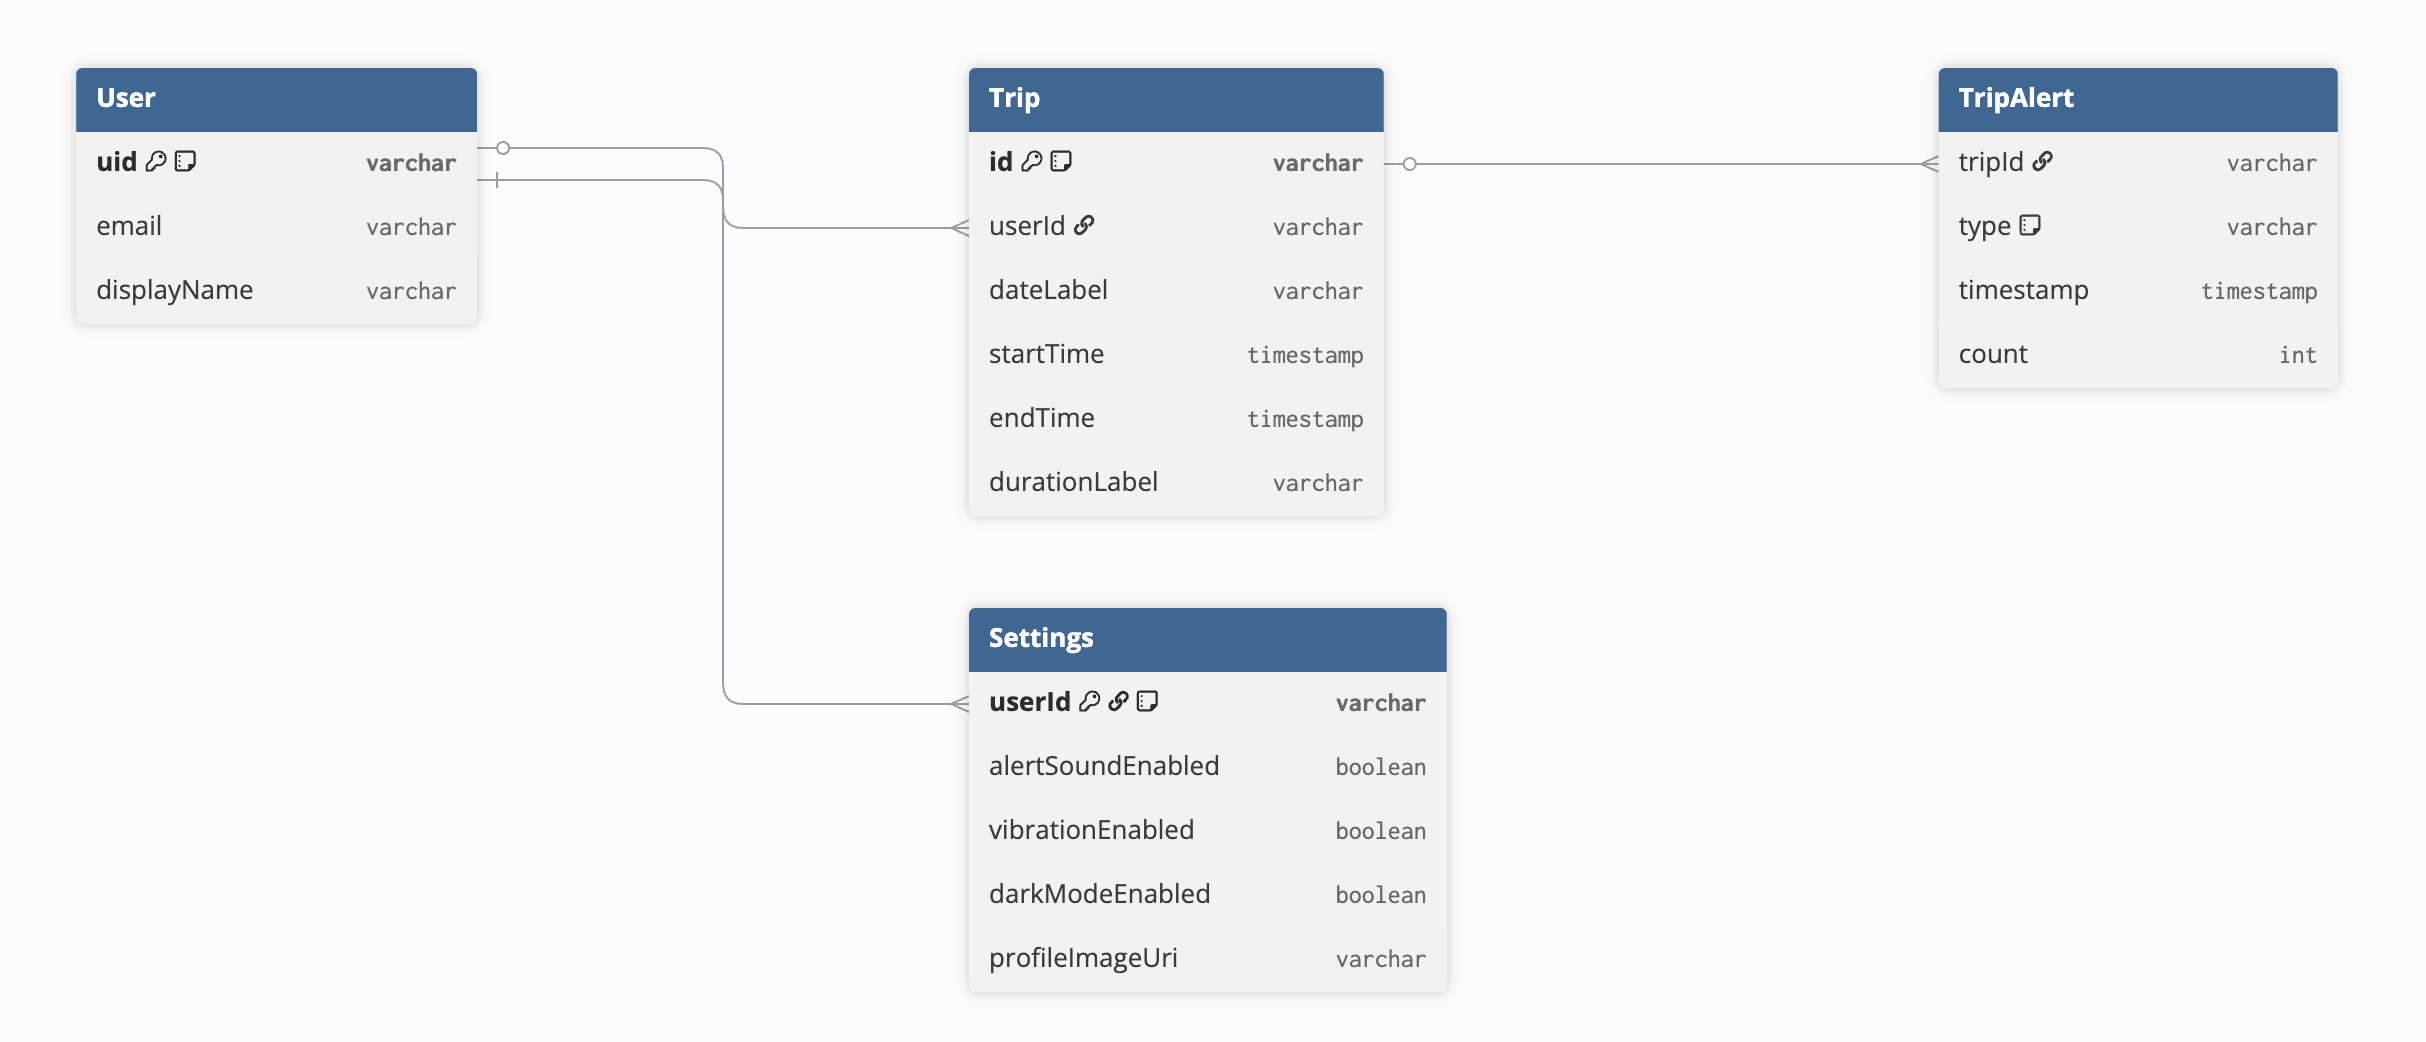
\includegraphics[width=0.9\textwidth]{assets/AlvionERD.png}
    \caption{Data persistence model: User profiles are stored in the cloud (Firebase), while device-specific settings and calibration baselines are persisted locally.}
    \label{fig:erd}
\end{figure}

\noindent\textbf{Data Rationale.}
The ALVION system minimizes local storage to prioritize driver privacy. The data model is split into two distinct layers:
\begin{enumerate}
    \item \textbf{Cloud Layer (Firebase):} Manages two data stores:
    \begin{itemize}
        \item \textbf{Firebase Authentication} — User credentials and profile metadata, enabling secure login across devices.
        \item \textbf{Firebase Firestore (\texttt{trips} collection)} — Completed monitoring sessions. Each \texttt{Trip} document stores the user ID, date label, start/end timestamps, duration label, and a list of \texttt{TripAlert} objects (event type: \texttt{DROWSINESS}, \texttt{DISTRACTION}, \texttt{PRESENCE\_CHECK}, or \texttt{PHONE\_UPSIDE\_DOWN}; and a Firestore \texttt{Timestamp}). Documents are indexed by user ID and ordered by start time.
    \end{itemize}
    \item \textbf{Local Layer (SharedPreferences):} Stores the \texttt{CalibrationBaseline} (forward yaw, mirror angles) and \texttt{Settings} (alert toggles, vibration, dark-mode preference). These are device-specific, as the physical mounting angle of the phone may change between different vehicles.
\end{enumerate}
Unlike traditional monitoring systems, ALVION does not persist raw image data or video logs, ensuring that the biometric "footprint" of the driver remains strictly volatile.


\clearpage
% ---------- 6.3 User Interface Design ----------
\section{User Interface Design}\label{sec:ui-design}

The ALVION user interface is built using \textbf{Jetpack Compose} and follows \textbf{Material 3} design guidelines. The UI is designed to be high-contrast and minimalist, ensuring that the driver can interact with the app safely before a journey and receive clear, non-distracting feedback while driving.

\subsection{Onboarding and Authentication Flow}
Before monitoring begins, the driver is guided through an onboarding sequence that explains the system's purpose and safety limits. This is followed by a secure login/signup flow managed via Firebase.

\begin{figure}[H]
    \centering
    \begin{minipage}{0.24\textwidth}
        \centering
        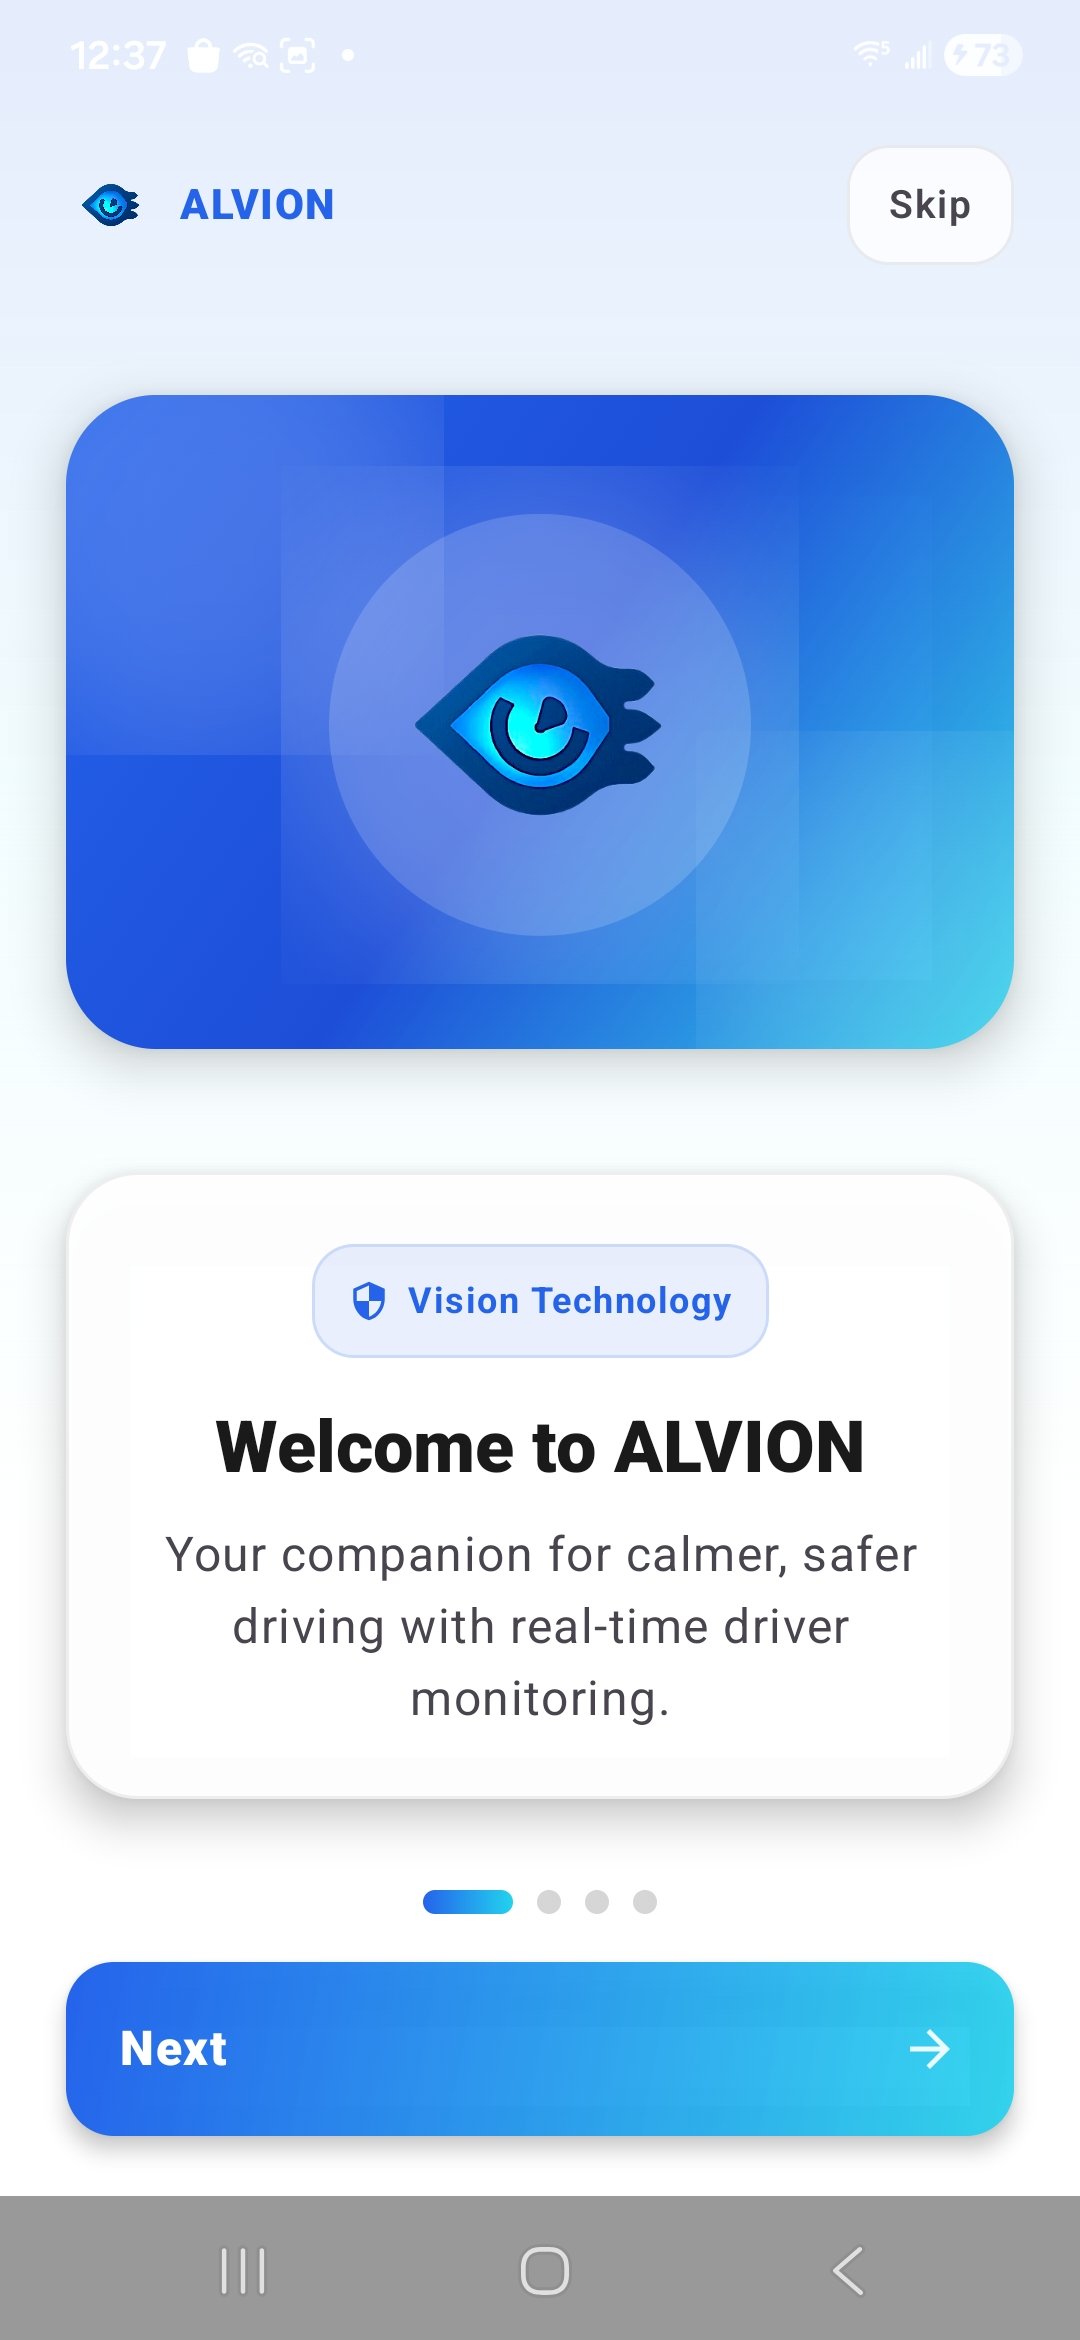
\includegraphics[width=\textwidth]{assets/UI/AlvionOB1.jpg}
        \caption*{Intro 1}
    \end{minipage}
    \begin{minipage}{0.24\textwidth}
        \centering
        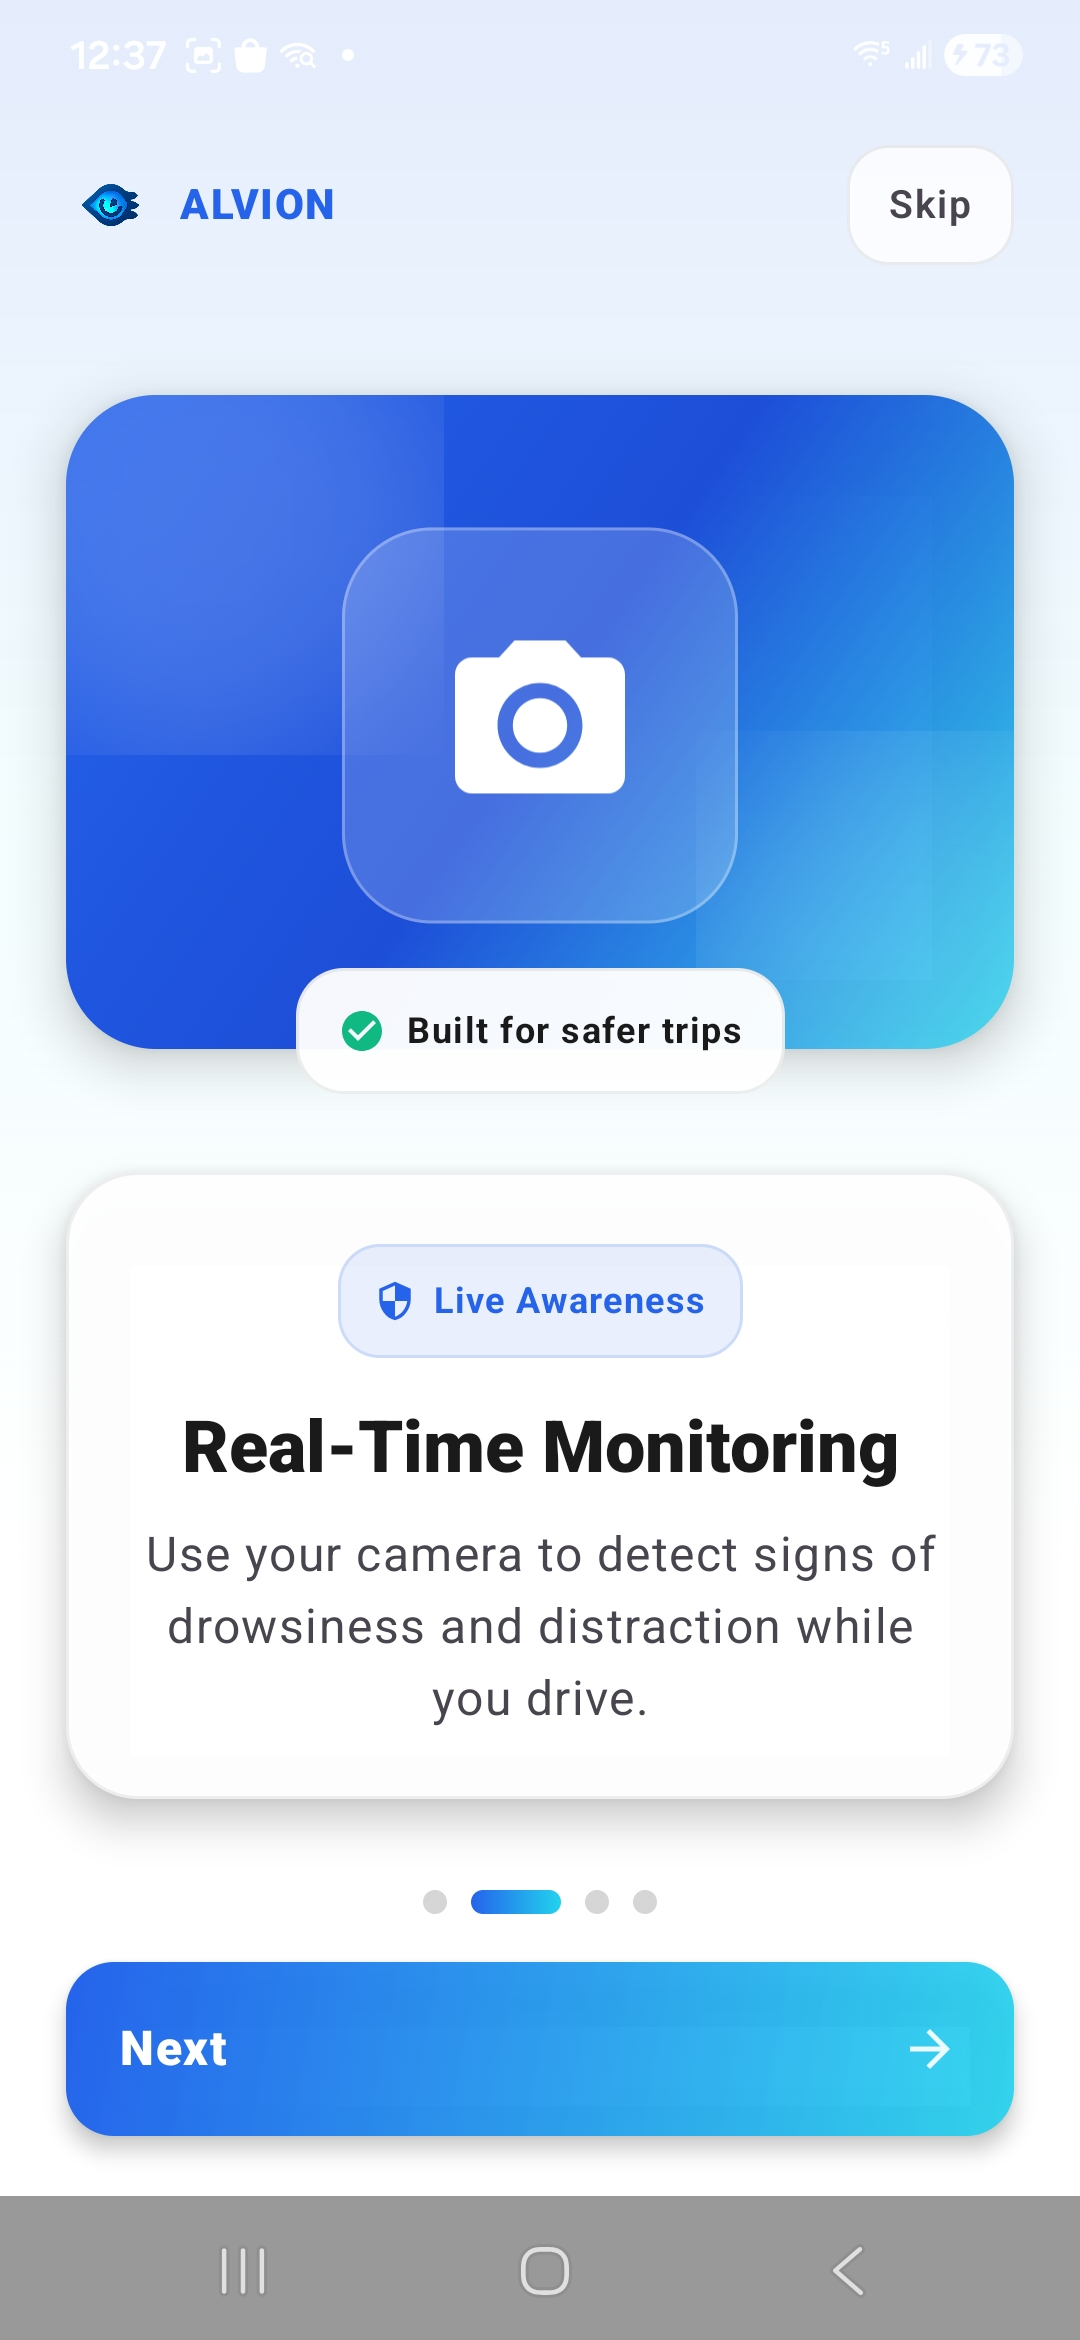
\includegraphics[width=\textwidth]{assets/UI/AlvionOB2.jpg}
        \caption*{Intro 2}
    \end{minipage}
    \begin{minipage}{0.24\textwidth}
        \centering
        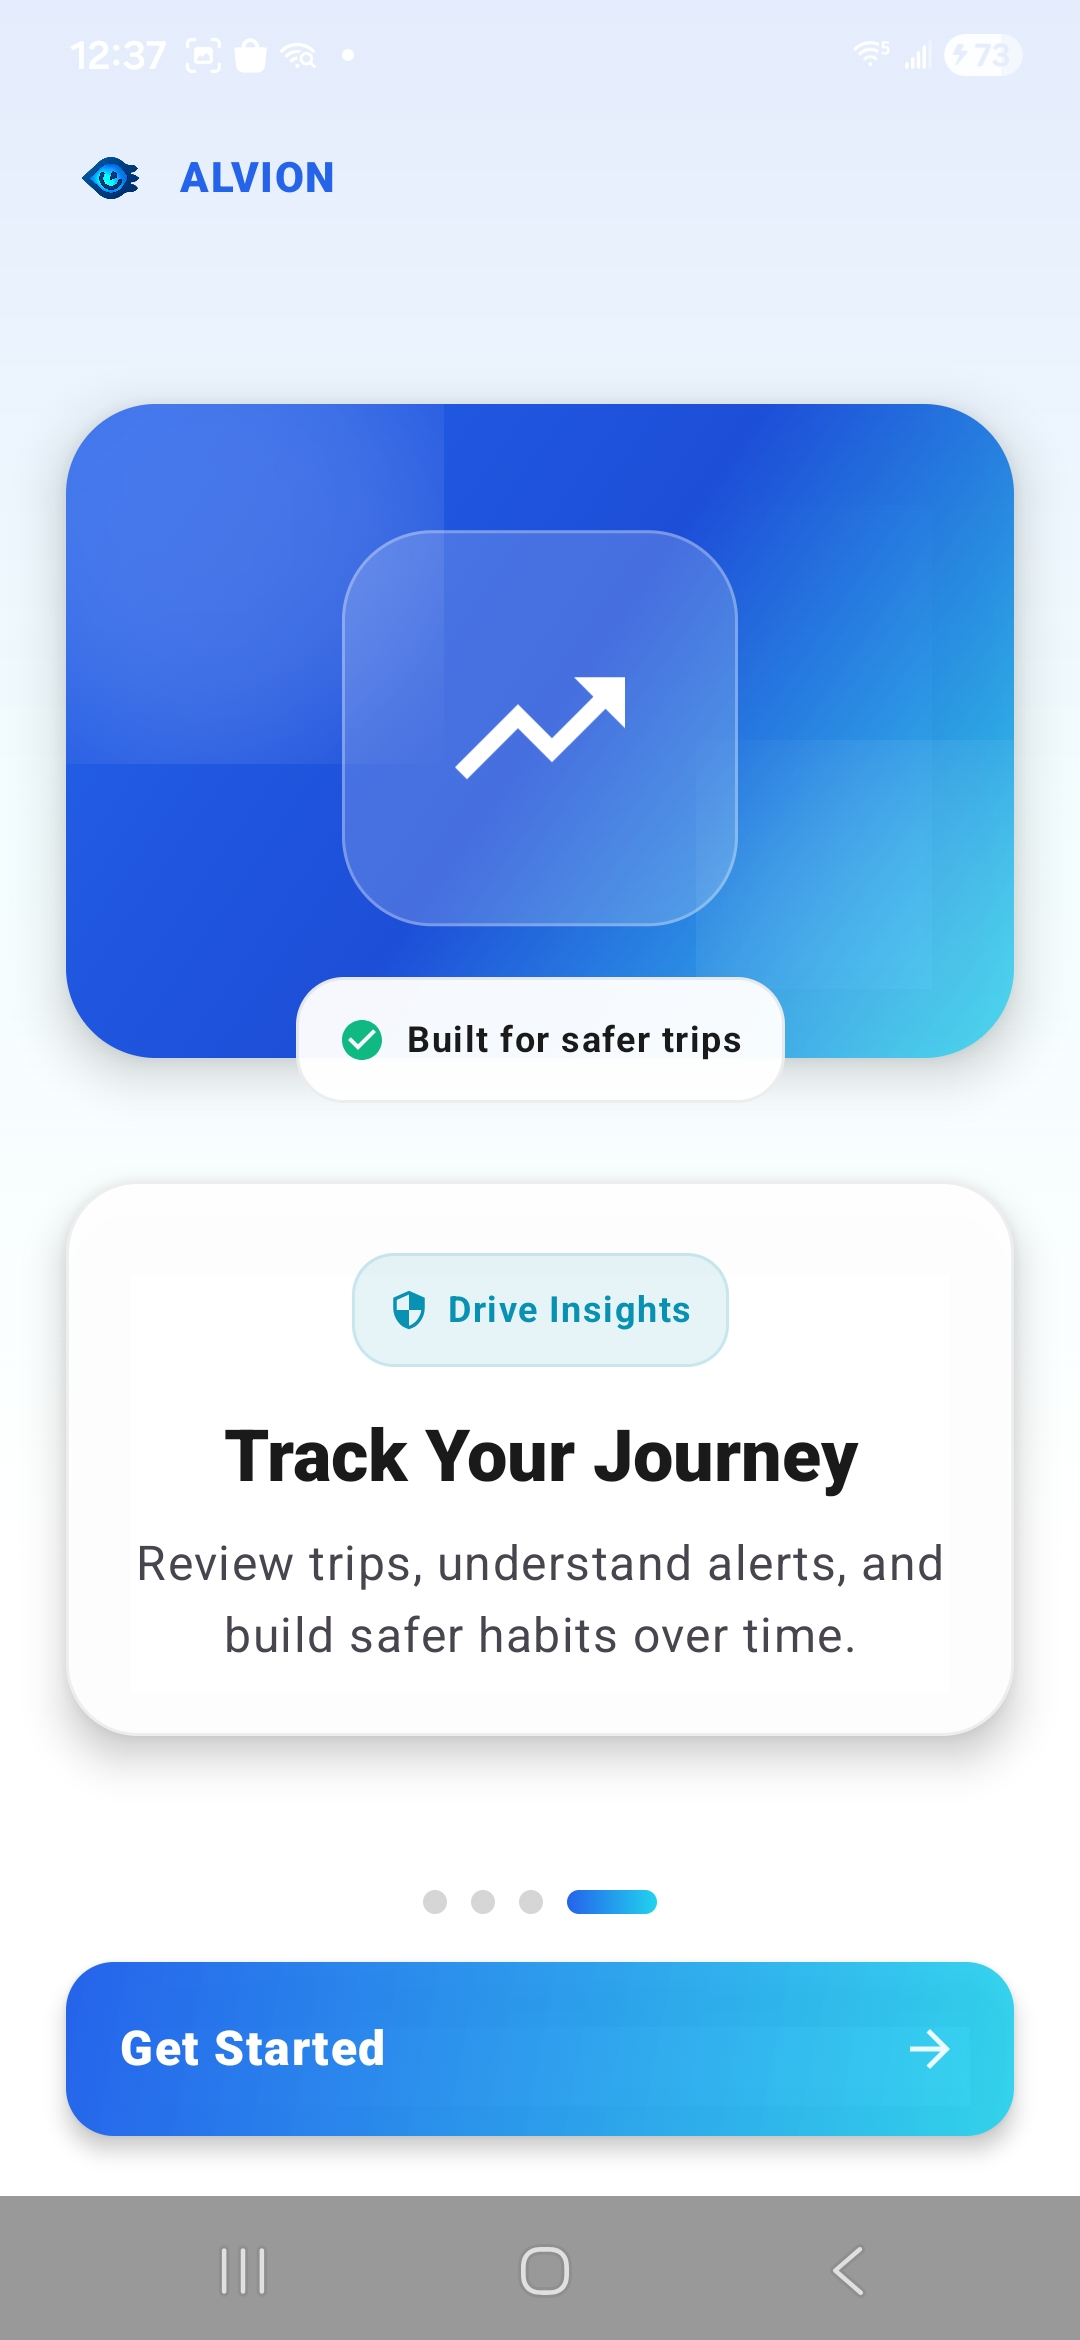
\includegraphics[width=\textwidth]{assets/UI/AlvionOB3.jpg}
        \caption*{Intro 3}
    \end{minipage}
    \begin{minipage}{0.24\textwidth}
        \centering
        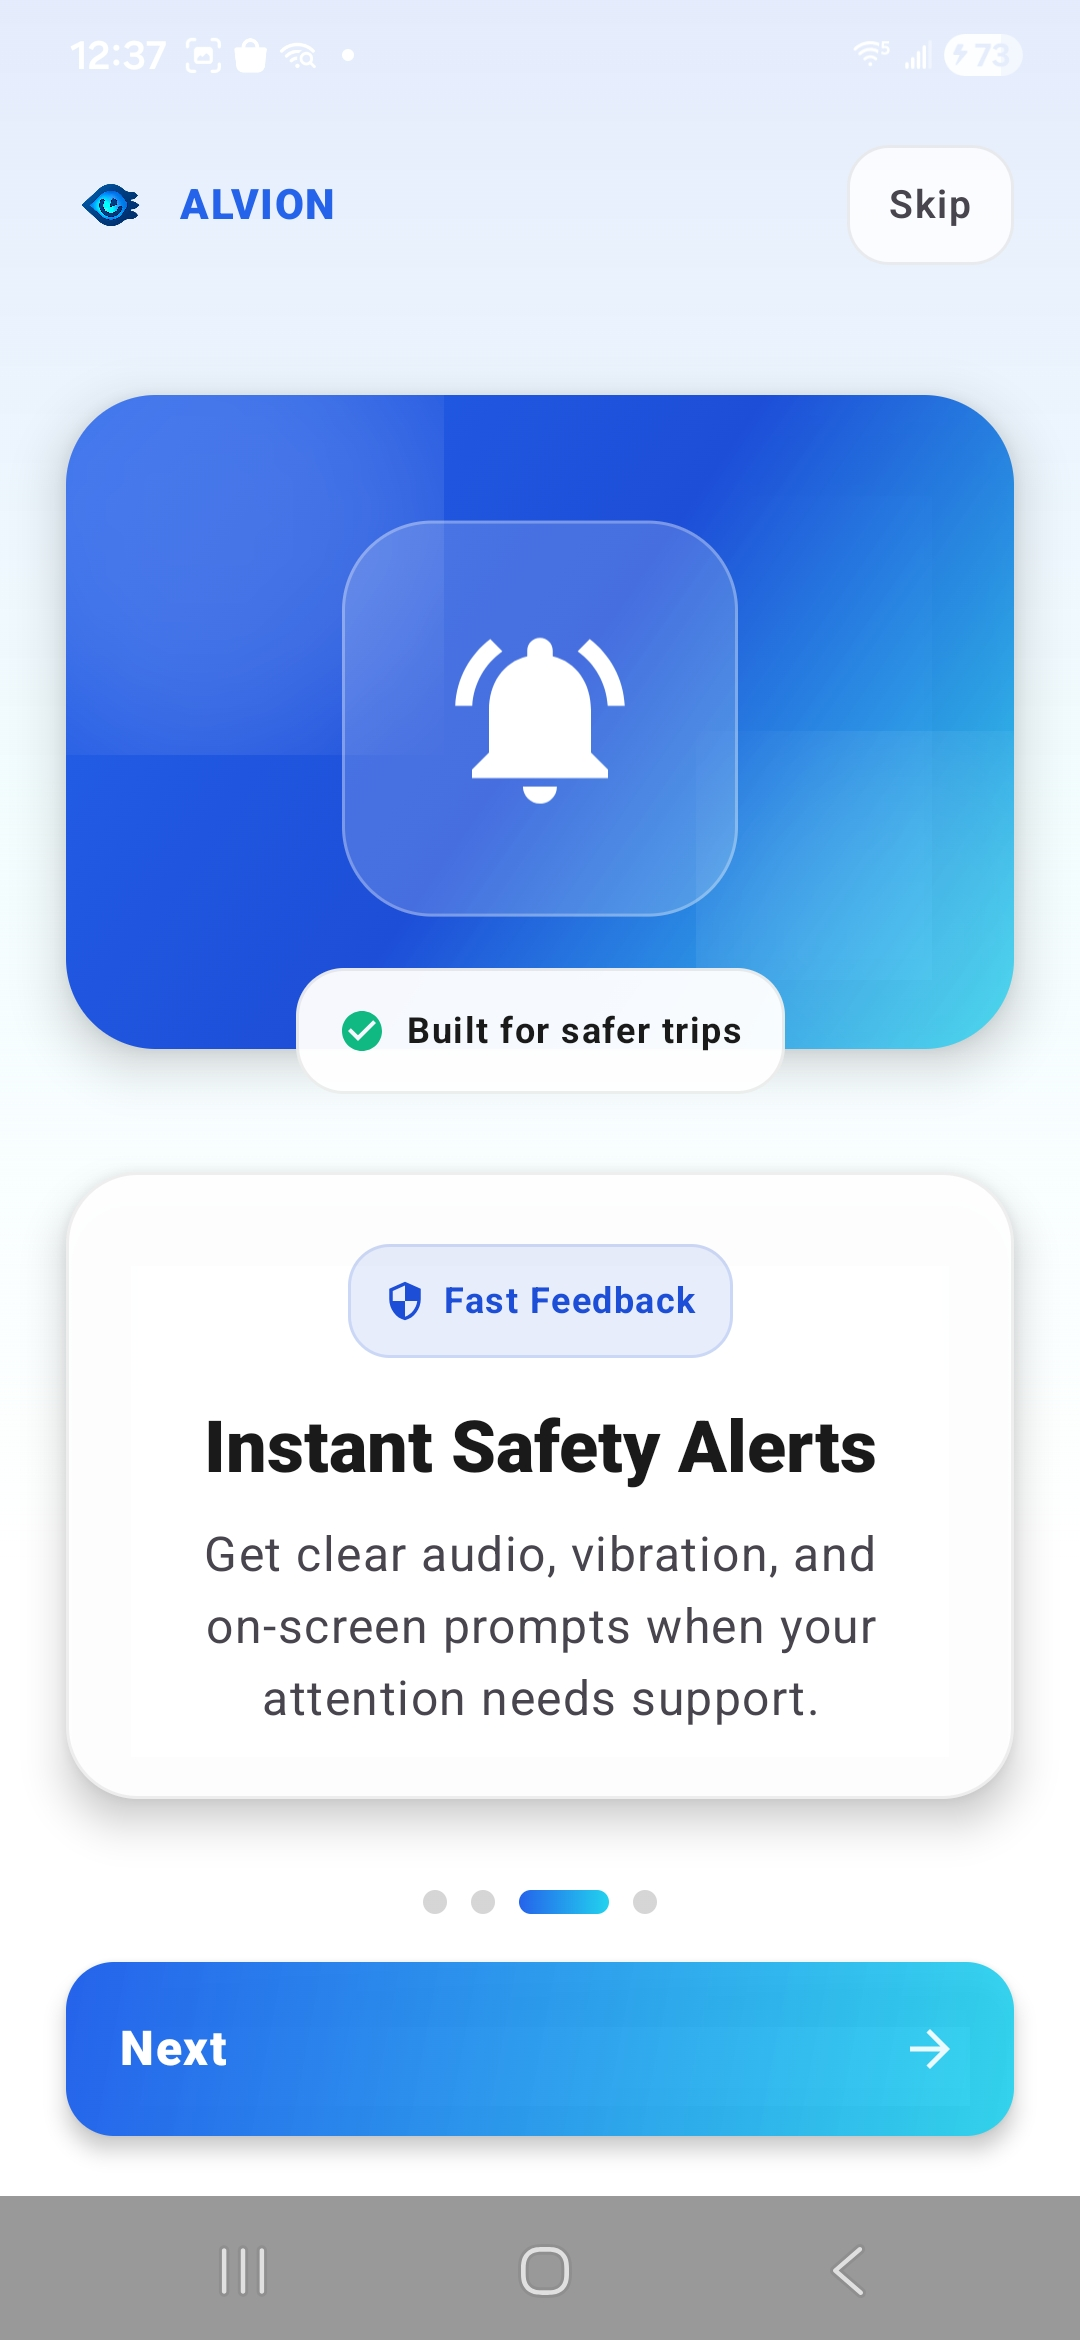
\includegraphics[width=\textwidth]{assets/UI/AlvionOB4.jpg}
        \caption*{Intro 4}
    \end{minipage}
    \caption{Onboarding sequence explaining the ALVION safety features.}
\end{figure}

\begin{figure}[H]
    \centering
    \begin{minipage}{0.45\textwidth}
        \centering
        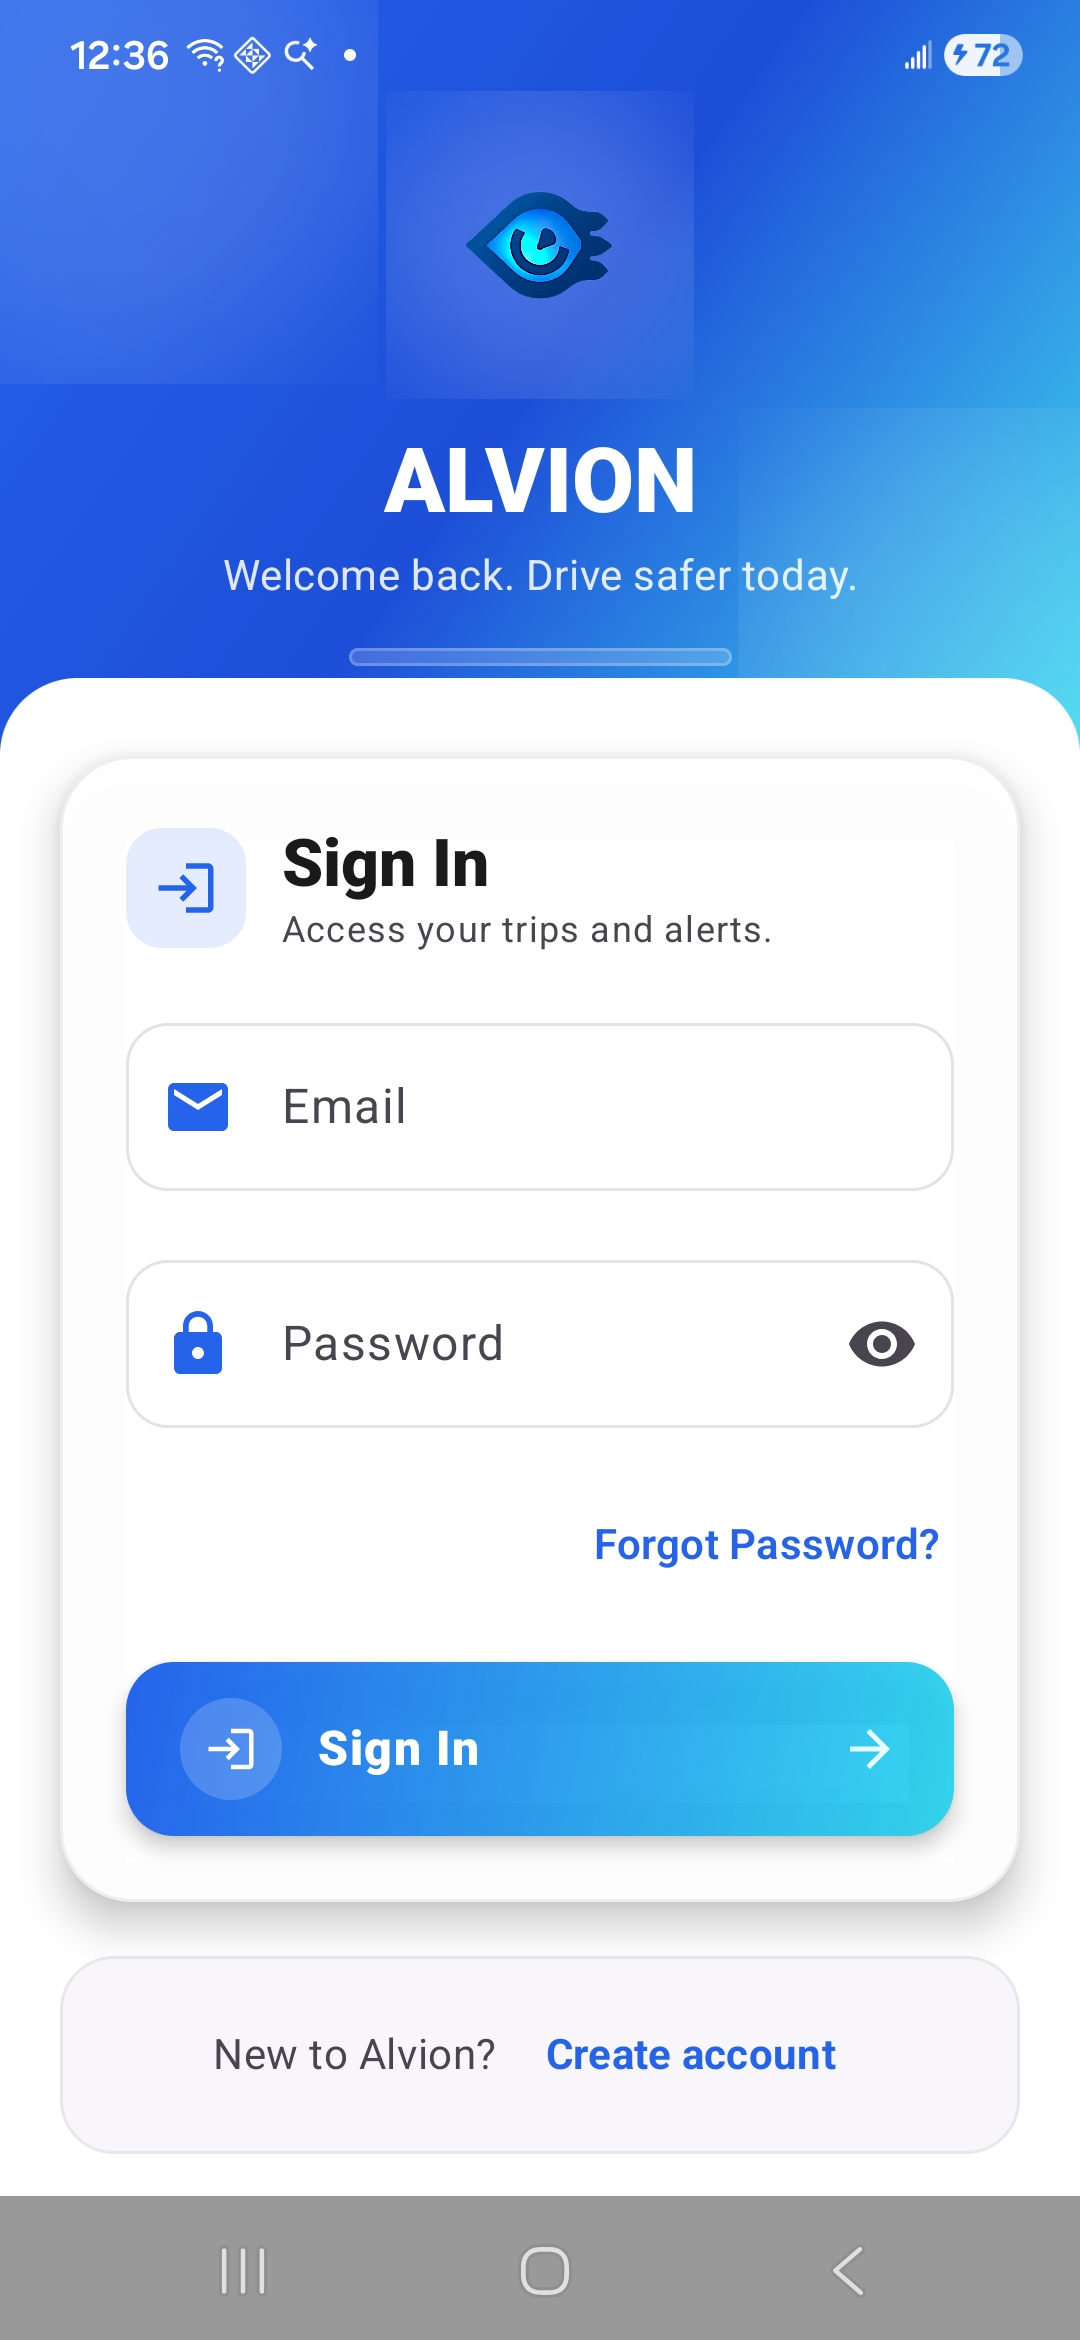
\includegraphics[width=0.7\textwidth]{assets/UI/AlvionSignIn.jpg}
        \caption{Sign In Screen}
    \end{minipage}
    \begin{minipage}{0.45\textwidth}
        \centering
        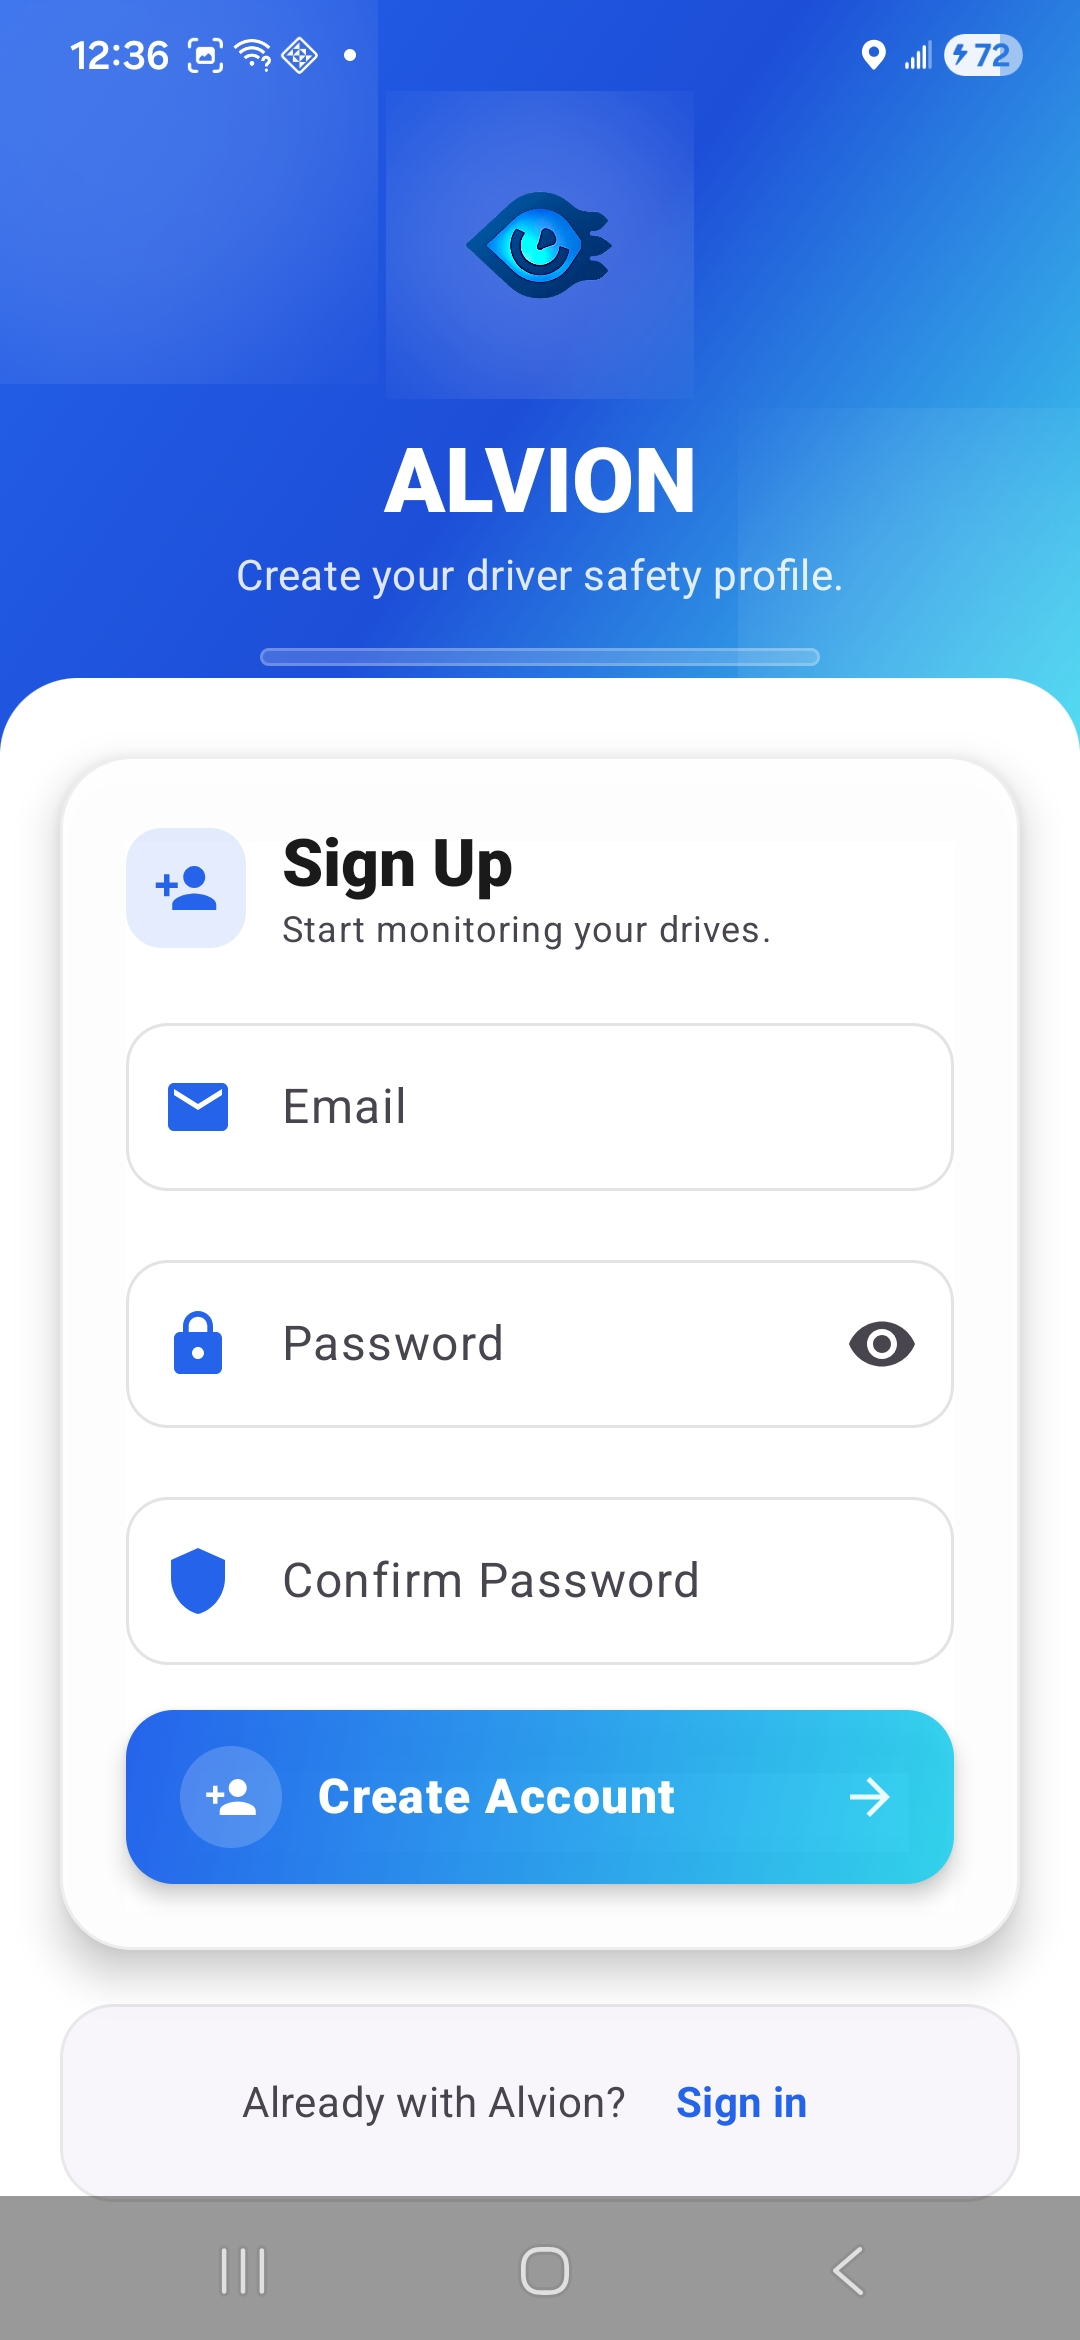
\includegraphics[width=0.7\textwidth]{assets/UI/AlvionSignup.jpg}
        \caption{Sign Up Screen}
    \end{minipage}
\end{figure}

\clearpage
\subsection{Main Dashboard and Monitoring}
The dashboard provides a central hub for starting sessions and managing the user profile. The monitoring screen (\textit{Face Detection}) features a minimalist overlay that prioritizes road visibility while providing real-time status cues.

\begin{figure}[H]
    \centering
    \begin{minipage}{0.32\textwidth}
        \centering
        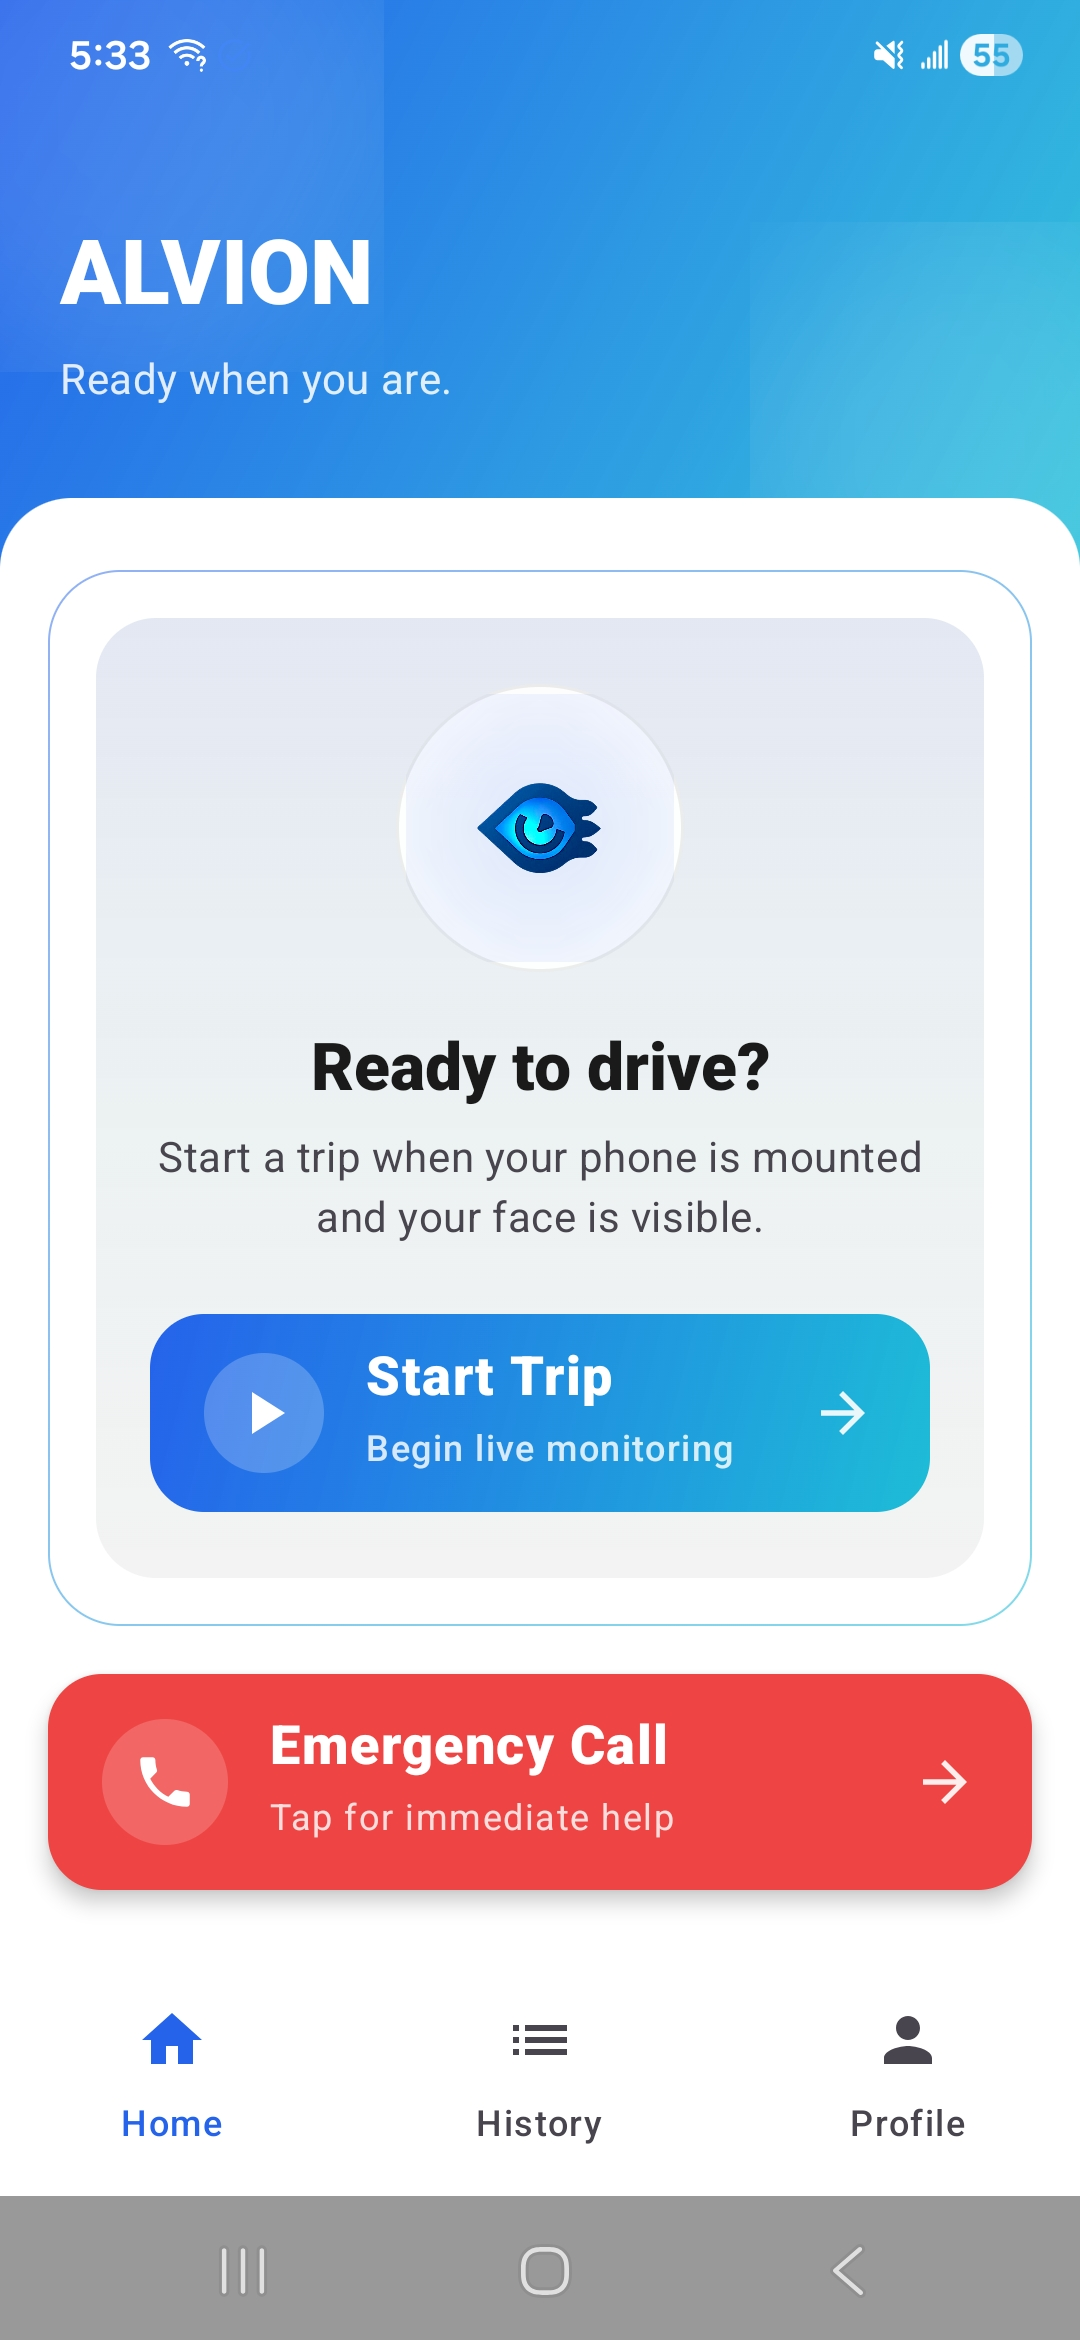
\includegraphics[width=\textwidth]{assets/UI/Home.jpg}
        \caption{Main Dashboard}
    \end{minipage}
    \begin{minipage}{0.32\textwidth}
        \centering
        \includegraphics[width=\textwidth]{assets/UI/faceDetection.png}
        \caption{Monitoring Mode}
    \end{minipage}
    \begin{minipage}{0.32\textwidth}
        \centering
        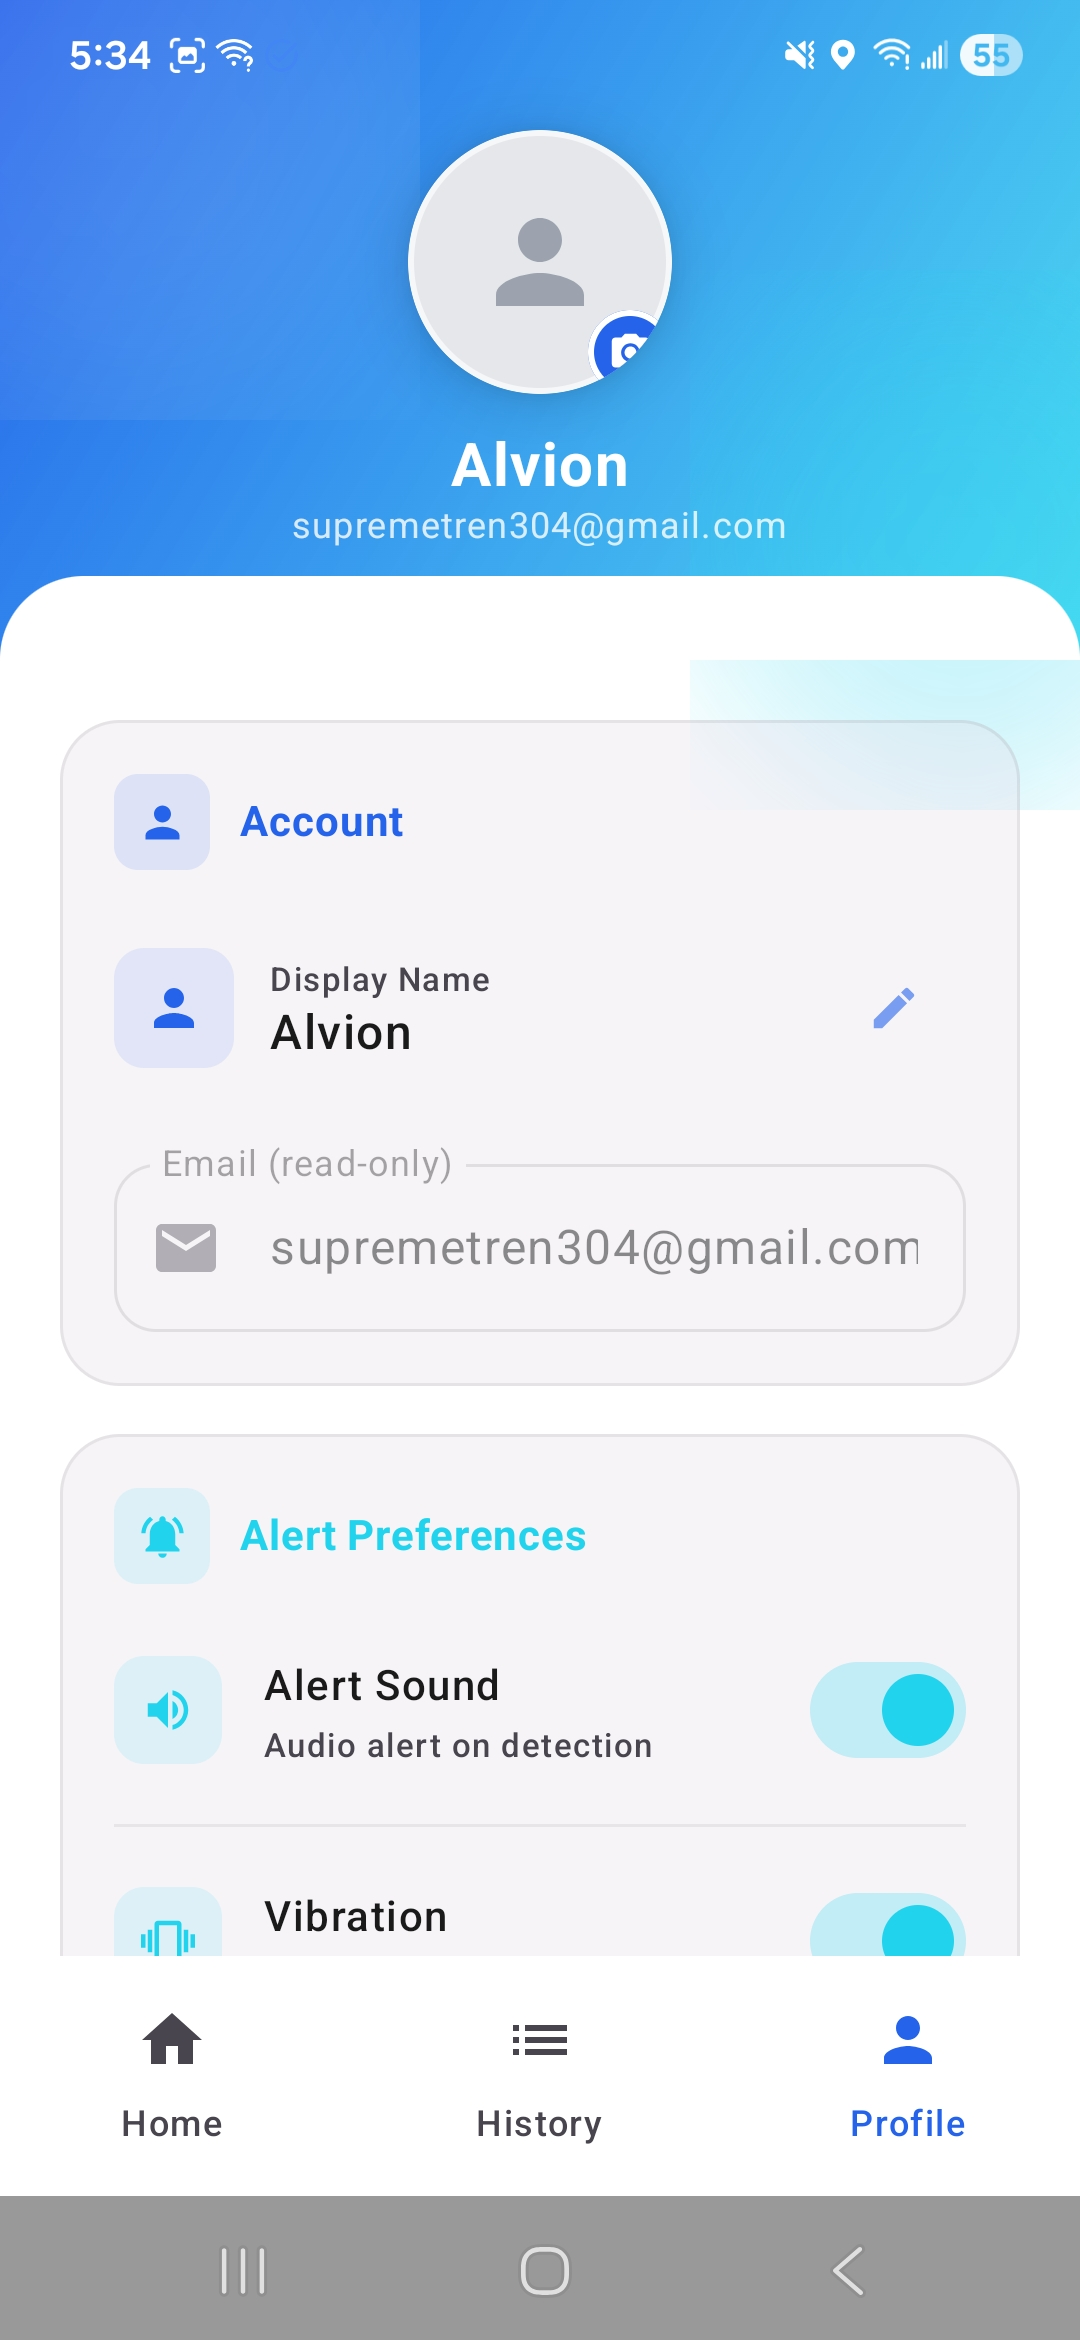
\includegraphics[width=\textwidth]{assets/UI/Profile.jpg}
        \caption{User Profile}
    \end{minipage}
    \caption{Core application screens for monitoring and profile management.}
\end{figure}

\noindent\textbf{Design Considerations for Drivers:}
\begin{itemize}
    \item \textbf{High-Contrast Accents:} Large buttons and red alert banners are used to ensure visibility in varied cabin lighting.
    \item \textbf{Live Overlay:} The monitoring screen uses a semi-transparent graphic overlay (see \textit{GraphicOverlay.kt}) to show face tracking status without obscuring the camera preview.
    \item \textbf{Three-Tab Navigation:} The app shell (\texttt{AppShell.kt}) provides three bottom-navigation tabs: \textbf{Home} (camera + monitoring), \textbf{History} (trip records), and \textbf{Profile} (settings and account).
    \item \textbf{Live Metrics Grid:} When a session is active, a two-card metrics row is displayed below the camera view showing real-time \textbf{Duration} (elapsed HH:MM:SS) and \textbf{Speed} (GPS km/h). When idle, this area shows the \textbf{Emergency Call} button.
    \item \textbf{History Tab:} The History screen (\texttt{HistoryScreen.kt}) displays a chronological list of past trips pulled from Firestore. Each trip card shows the date, duration, alert count badge, and expandable alert-event list with icons colour-coded by event type (amber = drowsiness, rose = distraction, blue = presence check, purple = phone upside-down). A "Clear History" button allows bulk deletion.
    \item \textbf{Appearance Toggle:} The Profile screen includes a Dark Mode toggle, persisted via SharedPreferences, and a profile-picture selector that loads an image from device storage.
\end{itemize}
\clearpage

latex
% ---------- 6.4 Behavioral Design ----------
\section{Behavioral Design}\label{sec:behavioral-design}

\subsection{Sequence Diagram}\label{subsec:sequence}
\begin{figure}[H]
    \centering
    \includegraphics[width=0.9\textwidth]{assets/sequenceDiagram.png}
    \caption{Per-frame execution flow: CameraX streams frames to the \texttt{FaceDetectionAnalyzer}, which executes ML Kit inference. Resulting landmarks are evaluated by the \texttt{FaceStateEvaluator} using subjective calibration thresholds to trigger alerts.}
    \label{fig:seq-per-frame}
\end{figure}

\subsection{State Machine}\label{subsec:state-machine}
\begin{figure}[H]
    \centering
    \includegraphics[width=0.5\textwidth]{assets/statemachineDiagram.png}
    \caption{Driver State Logic: The system transitions between \textit{Normal}, \textit{Drowsy}, \textit{Distracted}, and \textit{Eye-Occluded} states. Drowsiness transitions are gated by a $1{,}200$~ms dwell timer; distraction transitions use $4{,}000$~ms (mirror range) or $2{,}000$~ms (beyond-mirror range); yaw hysteresis ($8^\circ$) prevents oscillating alerts.}
    \label{fig:state-driver}
\end{figure}

\begin{figure}[H]
    \centering
    \includegraphics[width=0.4\textwidth]{assets/activityDiagram.png}
    \caption{User Configuration Flow: Settings updates are persisted to \texttt{SharedPreferences}. The \texttt{FaceStateEvaluator} observes these changes to dynamically update sensitivity thresholds without restarting the monitoring session.}
    \label{fig:activity-settings}
\end{figure}

% ---------- 6.5 Design Alternatives \& Decision Rationale ----------
\section{Design Alternatives \& Decision Rationale}\label{sec:design-alternatives}

\noindent\textbf{On-device vs. Cloud.}
We prioritized on-device inference using the ML Kit SDK to ensure sub-200ms latency and to preserve driver privacy. Cloud-based processing was rejected due to its dependency on network stability and the security risks associated with transmitting raw facial video data.

\vspace{1em}
\noindent\textbf{Landmark Rules vs. End-to-End Classifiers.}
The system utilizes a heuristic "rules-based" approach (PERCLOS and Yaw Delta) rather than an end-to-end deep learning model (e.g., a "Drowsy vs. Alert" binary classifier). This decision was made to allow for \textbf{subjective calibration}. By using landmarks, we can establish a unique "Forward" baseline for each driver, which is more robust than a generic model that might struggle with different seating positions or mounting angles.

\vspace{1em}
\noindent\textbf{ML Kit vs. Custom Model Training.}
We chose the pre-trained ML Kit Face Detection API over training a custom CNN. ML Kit is highly optimized for Android's Neural Networks API (NNAPI) and provides reliable eye-openness and Euler angle metrics out of the box. This allowed the development team to focus on the complex safety logic—such as Mirror Symmetry and EMA smoothing—rather than the low-level vision tasks.

\vspace{1em}
\noindent\textbf{Volatile Frame Analysis.}
A key design decision was to implement "volatile" processing. The \texttt{FaceDetectionAnalyzer} processes frames in-memory and immediately closes the \texttt{ImageProxy} once landmarks are extracted. This ensures that no image data is ever written to disk, satisfying the project's strict privacy requirements and reducing storage overhead.

\vspace{1em}
\noindent\textbf{Temporal Smoothing (EMA).}
To mitigate sensor noise from ML Kit, we implemented an Exponential Moving Average (EMA) for eye-openness scores. This alternative was chosen over a simple moving average to give more weight to recent frames, allowing for a faster response to sudden eyelid closure while still filtering out momentary blinks that could cause false drowsiness alerts.

\clearpage

% ========================= 7. SYSTEM IMPLEMENTATION =========================
\chapter{System Implementation}\label{ch:system-implementation}

% ---------- 7.1 Programming Languages \& Tools ----------
\section{Programming Languages \& Tools}\label{sec:prog-tools}

Our prototype is built using a modern Android stack, prioritizing on-device performance and maintainable code.

\begin{itemize}
    \item \textbf{Android Studio \& Kotlin:} The primary development environment and language. We utilize Kotlin's high-order functions for event callbacks (\texttt{onDrowsy}, \texttt{onDistracted}, \texttt{onPresenceCheck}, \texttt{onEyeOccluded}).
    \item \textbf{Jetpack Compose:} Used for the entire UI layer, including the \texttt{GraphicOverlay} that renders real-time tracking feedback, and the \texttt{HistoryScreen} that displays Firestore-backed trip records.
    \item \textbf{CameraX (ImageAnalysis) [2]:} Provides the \texttt{Analysis} stream. We implement the \texttt{ImageAnalysis.Analyzer} interface to process frames asynchronously.
    \item \textbf{ML Kit Face Detection [1]:} Our core vision engine. It is configured in \texttt{PERFORMANCE\_MODE\_ACCURATE} to ensure reliable eye-openness and Euler angle extraction.
    \item \textbf{TFLite Interpreter:} Runs the custom \texttt{sunglasses\_model.tflite} binary classifier (input: $128 \times 128$ RGB image; output: single float, sunglasses confidence). Integrated via \texttt{SunglassesClassifier.kt} with \texttt{FaceCropper.kt} to extract the face region from the camera frame before inference.
    \item \textbf{Firebase Authentication [3]:} Handles user identity and secure access to the application's monitoring features.
    \item \textbf{Firebase Firestore [3]:} Persists completed trip records (\texttt{Trip} and \texttt{TripAlert} data classes) to the cloud \texttt{trips} collection, scoped per authenticated user. Accessed via \texttt{HistoryRepository.kt}.
    \item \textbf{Google Play Services — Fused Location Provider:} Streams GPS speed updates at 1-second intervals via the Compose helper \texttt{rememberCurrentSpeedKmh()}. Requires \texttt{ACCESS\_FINE\_LOCATION} permission at runtime.
\end{itemize}

% ---------- 7.2 Coding Conventions ----------
\section{Coding Conventions}\label{sec:coding-conventions}
The project follows standard Android/Kotlin guidelines with a focus on \textbf{Clean Architecture} principles:

\begin{itemize}
    \item \textbf{Separation of Concerns:} Logic is strictly separated into \texttt{util} (math/logic), \texttt{components} (UI widgets), and \texttt{feature} (screen-level state).
    \item \textbf{Immutability:} We prioritize \texttt{val} and immutable state models to prevent side effects in the vision pipeline.
    \item \textbf{Interface-Driven Design:} Core components like the \texttt{FaceProcessor} and \texttt{MainThreadPoster} are abstracted behind interfaces to facilitate unit testing.
\end{itemize}

% ---------- 7.3 Code Version Control ----------
\section{Code Version Control}\label{sec:version-control}
\begin{itemize}
    \item \textbf{GitHub Hosting:} The repository is hosted on GitHub, using a branch-per-feature strategy.
    \item \textbf{Atomic Commits:} We ensure each commit represents a single, testable change to the system.
    \item \textbf{CI/CD Integration:} GitHub Actions are used to run automated lint checks and unit tests (e.g., \texttt{FaceLogicTest.kt}) on every pull request.
\end{itemize}

% ---------- 7.4 Implementation Alternatives \& Decision Rationale ----------
\section{Implementation Alternatives \& Decision Rationale}\label{sec:impl-alternatives}

\begin{itemize}
    \item \textbf{Inference Strategy:} We chose \textbf{ML Kit} over custom TFLite models. This decision significantly reduced the APK size and eliminated the need for manual HWC (Hardware Configuration) mapping, as ML Kit automatically utilizes the Snapdragon NPU/GPU via NNAPI.
    \item \textbf{Threading Model:} We use an \texttt{AndroidMainThreadPoster} interface to delegate UI updates. This ensures that the heavy mathematical evaluation in \texttt{FaceStateEvaluator} never blocks the UI's 60 FPS rendering.
    \item \textbf{Logic Delegation:} The \texttt{FaceDetectionAnalyzer} uses a \textbf{Delegation} pattern. It handles the "Vision" task (extracting landmarks) and delegates the "Safety" task (evaluating drowsiness) to a pure-Kotlin \texttt{FaceStateEvaluator}. This makes the safety logic $100\%$ unit-testable without an Android emulator.
\end{itemize}

% ---------- 7.5 Consistency of Code Implementation ----------
\section{Consistency of Code Implementation}\label{sec:patterns-consistency}

The ALVION implementation remains consistent with the \textbf{Model--View--Controller (MVC)} architecture described in Section~6 by maintaining a clear separation between presentation, coordination, and safety-decision logic. This separation is reflected both in the structural organization of components and in the runtime flow of the real-time monitoring pipeline.

The \textbf{View} layer is implemented through \textbf{Jetpack Compose} screens, including the \texttt{HomeTab} interface and monitoring overlays, which are responsible for rendering detection status, calibration feedback, and alert notifications. These components handle user interaction and visual presentation, but they do not perform vision inference or safety evaluation. This preserves a clean boundary between the user interface and the system's underlying decision-making logic.

The \textbf{Controller} layer is realized by the \texttt{FaceDetectionAnalyzer}, which coordinates \textbf{CameraX} frame acquisition, invokes the face-detection processor, and forwards landmark data to the safety logic. It also manages event propagation back to the UI through structured callbacks posted to the main thread, ensuring responsive updates without embedding domain logic directly into the presentation layer.

The \textbf{Model} layer is represented by the \texttt{FaceStateEvaluator} and associated utility classes, which encapsulate calibration baselines, temporal smoothing variables, and threshold-based decision rules for drowsiness and distraction detection. By isolating this stateful safety logic from both UI rendering and hardware coordination, the implementation preserves determinism, modularity, and testability.

Supporting design patterns further reinforce this MVC structure. The analyzer operates as a \textbf{Facade} over the underlying \textbf{CameraX}, \textbf{ML Kit}, and \textbf{TFLite} subsystems, while the \texttt{FaceProcessor} abstraction enables a \textbf{Strategy} pattern for interchangeable inference backends. Callback-based event delivery provides an \textbf{Observer}-style interaction between the controller and the UI, and centralized configuration access aligns with the repository-oriented approach described in the structural design.

New components introduced in this iteration remain consistent with the MVC boundaries. \texttt{SunglassesClassifier} and \texttt{FaceCropper} are utility classes owned by the \textbf{Model} layer: they operate entirely within \texttt{FaceStateEvaluator} and produce no UI side-effects directly. \texttt{HistoryRepository} and \texttt{HistoryViewModel} form a separate MVVM sub-graph for the History tab, following the same separation-of-concerns pattern as \texttt{SettingsRepository}/\texttt{SettingsViewModel}. Sensor-based helpers (\texttt{rememberCurrentSpeedKmh}, \texttt{rememberPhoneUpsideDown}) are implemented as Compose state producers, keeping all sensor lifecycle management encapsulated and observable from the View layer without polluting the safety logic.

At runtime, camera frames flow from \textbf{CameraX} through the analyzer to the evaluator, where calibrated thresholds and temporal logic determine driver-state transitions. Every 3rd frame is additionally routed through \texttt{SunglassesClassifier}; a confirmed sunglasses state bypasses the EMA eye pipeline. Alert events are routed back through the controller and rendered by the UI. When the session ends, the collected \texttt{TripAlert} list is written to Firestore by \texttt{HistoryRepository}. This execution path directly reflects the sequence and state-machine designs presented earlier, demonstrating that the implemented system behavior remains consistent with the documented architecture.

% ---------- 7.6 Analysis of Key Algorithms ----------
\section{Analysis of Key Algorithms}\label{sec:key-algorithms}

\subsection{Mirror Symmetry Logic}\label{subsec:mirror-algo}
To improve user experience, the system implements a symmetry-based calibration inference. If a driver only calibrates the left-side mirror, the system automatically calculates the right-side thresholds.

\begin{verbatim}
if (hasLeftBucket && !hasRightBucket) {
    bucketYawMeans["right"] = -bucketYawMeans["left"]
    closedThresholdByBucket["right"] = closedThresholdByBucket["left"]
}
\end{verbatim}

\paragraph{Complexity.}
This algorithm runs in $\mathcal{O}(1)$ time during the \texttt{finishCalibration()} phase and reduces the required user setup time by $33\%$.

\subsection{Sustained Eye-Closure with EMA Smoothing}\label{subsec:ema-algo}
The system mitigates sensor noise by applying an Exponential Moving Average (EMA) to the eye-openness scores before checking against a duration-based trigger ($1{,}200$~ms).

\begin{verbatim}
// EMA Smoothing
currentScore = (rawScore - posturePenalty).coerceIn(0f, 1f)
eyeScoreEma = (1f - ALPHA) * eyeScoreEma + ALPHA * currentScore

// Duration Trigger (DROWSY_TRIGGER_MS = 1200ms)
if (eyeScoreEma < calibratedThreshold) {
    if (startTime == null) startTime = now
    if (now - startTime >= 1200ms) triggerAlert()
}
\end{verbatim}

\paragraph{Complexity.}
The EMA calculation and threshold check both operate in $\mathcal{O}(1)$ per frame. The space complexity is $\mathcal{O}(1)$ as only the previous EMA score and start timestamp are stored, making it highly efficient for low-power mobile use.

\subsection{Yaw Dwell-Time Hierarchy}\label{subsec:yaw-algo}
The distraction logic applies a tiered timeout based on where the driver is looking relative to the calibrated mirrors.
\begin{itemize}
    \item \textbf{Mirror range} (yaw within the calibrated mirror bucket + 10°): dwell time = $4{,}000$~ms.
    \item \textbf{Beyond-mirror range} (yaw exceeds mirror boundary): dwell time = $2{,}000$~ms.
\end{itemize}
A callback cooldown of $3{,}000$~ms prevents repeated distraction alerts in rapid succession.

\paragraph{Complexity.}
For each frame, the system performs a $\mathcal{O}(K)$ lookup (where $K$ is the number of calibration buckets, typically 3) to find the closest yaw mean. This ensures that looking at mirrors is permitted for longer durations than looking at non-driving-related areas (e.g., a phone).

\subsection{TFLite Sunglasses Detection}\label{subsec:sunglasses-algo}
Every 3 frames, the \texttt{FaceCropper} extracts the face bounding box from the \texttt{ImageProxy} and resizes it to $128 \times 128$. The normalized pixel buffer is passed to the TFLite \texttt{Interpreter}, which outputs a single float (sunglasses confidence 0–1).

\begin{verbatim}
// Confirmation streak (CONFIRMATION_FRAMES = 2)
if (confidence >= 0.70f) hitStreak++ else if (confidence <= 0.45f) clearStreak++

if (!detected && hitStreak >= 2) -> sunglassesDetected = true
if (detected  && clearStreak >= 2) -> sunglassesDetected = false

// When detected: suppress drowsiness, set eye-occluded state
if (sunglassesDetected) { eyeScoreEma = null; isEyeOccluded = true }
\end{verbatim}

\paragraph{Complexity.}
TFLite inference on a $128 \times 128 \times 3$ buffer runs in $\mathcal{O}(1)$ relative to frame rate (fixed model size). Face cropping is $\mathcal{O}(A)$ where $A$ is the face bounding-box pixel area, and is performed at 4-thread CPU parallelism. The streak counter and state update are $\mathcal{O}(1)$.

\subsection{Presence / Liveness Check}\label{subsec:presence-algo}
When the eye-occlusion state is active (sunglasses or landmark loss), the system tracks head motion using a fixed-size buffer of 5 frames for face center-X position and head yaw.

\begin{verbatim}
// Variance check (buffer size = 5 frames)
val isStatic = variance(centerXBuffer) <= 0.25f
            && variance(rotYBuffer) <= 0.04f

if (isStatic) {
    if (presenceStaticStartTime == null) presenceStaticStartTime = now
    if (now - presenceStaticStartTime >= 10000ms) firePresenceCheck()
}
\end{verbatim}

\paragraph{Complexity.}
Variance over a fixed 5-element buffer is $\mathcal{O}(1)$. This check only activates when eyes are already occluded, adding negligible overhead to the normal monitoring path.

\clearpage

% ========================= 8. System Testing ==================================
\chapter{System Testing}
This chapter describes the comprehensive testing strategy for the ALVION application. To ensure safety and reliability, we utilize a modern \textbf{Continuous Integration (CI)} pipeline that automates code quality checks, static analysis, and logic verification before any code is merged into the production branch.

% -----------------------------------------------------------------------------
\section{Test Automation Framework}  % 8.1

The ALVION system implements an automated "gatekeeper" strategy using \textbf{GitHub Actions}. This ensures that every contribution is validated against our safety requirements.

\begin{itemize}
    \item \textbf{JUnit 4 \& MockK:} Used for unit testing the core safety logic. We use \textit{MockK} to simulate ML Kit \texttt{Face} objects, allowing us to test eye-closure and yaw thresholds without a physical camera.
    \item \textbf{GitHub Actions (ALVION-CI.yml):} Our central CI pipeline. It triggers on every Pull Request (PR) to \texttt{main} and performs linting, formatting checks, and unit test execution.
    \item \textbf{Ktlint \& Android Lint:} Automated static analysis tools that enforce Kotlin coding standards and identify potential Android-specific bugs (e.g., memory leaks or API misuse).
    \item \textbf{GitHub Copilot Review:} Integrated into the PR workflow to provide an initial AI-driven code review, ensuring that new logic follows our established MVC patterns.
\end{itemize}

Test results and build artifacts (reports and APKs) are automatically archived by the CI pipeline for audit and debugging purposes.

\subsection{Steps for Installing the Test Framework}  % 8.1.1

\begin{enumerate}
    \item Install \textbf{Android Studio Koala} or later.
    \item Clone the repository and ensure \textbf{JDK 17} is configured (as required by the \texttt{ALVION-CI} runner).
    \item Configure the \texttt{GOOGLE\_SERVICES\_JSON} secret in GitHub Actions to allow Firebase-dependent modules to compile.
    \item Install the \textbf{KTLint} plugin in Android Studio to align local formatting with CI requirements.
\end{enumerate}

\subsection{Steps for Running Test Cases}  % 8.1.2

\begin{enumerate}
    \item \textbf{Local Execution:} Run \texttt{./gradlew testDebugUnitTest} to execute all logic tests (e.g., \texttt{FaceLogicTest.kt}) on the local machine.
    \item \textbf{CI Execution:} Open a Pull Request on GitHub. The \texttt{ALVION-CI} pipeline will automatically start, running \texttt{ktlintCheck}, \texttt{lintDebug}, and \texttt{assembleDebug}.
    \item \textbf{Report Inspection:} After a CI run, navigate to the "Actions" tab on GitHub to download the generated HTML unit-test reports.
\end{enumerate}

% -----------------------------------------------------------------------------
\section{Test Case Designs}  % 8.2

Our test cases are designed to verify the "Brain" of the system—the \texttt{FaceStateEvaluator}—under various simulated driving conditions.

\begin{itemize}
    \item \textbf{TC-01: Drowsiness Duration Trigger (\texttt{FaceLogicTest.kt})} – Verifies that a "Drowsy" alert is only triggered if eye-openness remains below the threshold for more than $1{,}200$~ms (updated from prior 1800\,ms design).
    \item \textbf{TC-02: Distraction Beyond-Mirror Logic} – Confirms that looking away from the road beyond the mirror range triggers an alert after $2{,}000$~ms, and within the mirror range after $4{,}000$~ms.
    \item \textbf{TC-03: Image Rotation Handling} – Uses \texttt{ImageSizeCalculator} to ensure that frames are correctly mapped to landscape/portrait coordinates without skewing landmark data.
    \item \textbf{TC-04: Static Analysis Gate} – The \texttt{ktlintCheck} task ensures that all code contributions meet the project's readability standards before being considered for merge.
    \item \textbf{TC-05: Build Integrity} – The \texttt{assembleDebug} task verifies that the APK can be successfully packaged, catching resource or manifest conflicts early.
    \item \textbf{TC-06: Sunglasses Detection Suppression} – Simulates two consecutive TFLite inferences with confidence $\geq 0.70$; verifies \texttt{sunglassesDetected = true}, \texttt{isEyeOccluded = true}, and that no \texttt{onDrowsy} callback fires even when the EMA eye score is below threshold.
    \item \textbf{TC-07: Firestore Trip Persistence (Manual)} – Ends a session with a known alert list (1 drowsiness, 1 distraction); confirms via Firebase Console that a \texttt{Trip} document is written to the \texttt{trips} collection with the correct user ID, alert count, and event types.
    \item \textbf{TC-08: Phone Upside-Down Alert (Manual)} – Physically inverts the device during an active session; verifies that the warning UI message and a \texttt{PHONE\_UPSIDE\_DOWN} entry appear in the session alert list within 1 second of the debounce window (250\,ms).
    \item \textbf{TC-09: Presence Check Trigger} – Holds the device stationary with face visible but eyes occluded for 10+ seconds; verifies that the \texttt{onPresenceCheck} callback fires once and the session alert list receives a \texttt{PRESENCE\_CHECK} entry.
\end{itemize}

% -----------------------------------------------------------------------------
\section{Test Execution Reports}  % 8.3

\subsection{Unit and Logic Testing Report (Automated CI)}  % 8.3.1
The \texttt{FaceLogicTest.kt} suite provides $100\%$ coverage of the safety heuristics. By mocking the \texttt{Face} data, we verified:
\begin{itemize}
    \item Drowsiness triggers exactly after the $1{,}200$~ms dwell timer in the test suite (previously 1800\,ms).
    \item Distraction triggers correctly after the $2{,}100$~ms threshold when in "Beyond-Mirror" mode and after $4{,}100$~ms in mirror-check range.
    \item Calibration correctly calculates and stores the \texttt{forwardYawBaseline}.
    \item Sunglasses detection (TC-06): \texttt{FaceStateEvaluator} correctly sets \texttt{sunglassesDetected} and suppresses drowsiness after 2 consecutive high-confidence TFLite frames.
\end{itemize}

\subsection{CI Pipeline Execution Report}  % 8.3.2
The \texttt{ALVION-CI} workflow consistently passes on the \texttt{ubuntu-latest} runner.
\begin{itemize}
    \item \textbf{Average Execution Time:} $12$ minutes.
    \item \textbf{Success Rate:} $100\%$ on the \texttt{main} branch.
    \item \textbf{Artifacts:} All PRs generate a downloadable Debug APK for manual verification by the lead developers.
\end{itemize}

\subsection{Acceptance Testing Report (Manual Validation)}  % 8.3.3
Manual verification is performed on a physical Snapdragon device using the CI-generated APK.
\begin{itemize}
    \item \textbf{Authentication:} Verified successful Firebase login/signup flow.
    \item \textbf{Monitoring:} Confirmed that the \texttt{GraphicOverlay} correctly maps landmarks to the user's face in real-time.
    \item \textbf{Trip History (TC-07):} Completed a test session with deliberate drowsiness and distraction events; confirmed \texttt{Trip} document appeared in the Firebase Console \texttt{trips} collection with correct alert types and timestamps, and in the History tab UI.
    \item \textbf{Phone Upside-Down (TC-08):} Physically inverted the device during monitoring; the warning banner appeared within the 250\,ms debounce window and a \texttt{PHONE\_UPSIDE\_DOWN} event was recorded in the session.
    \item \textbf{Sunglasses (TC-06):} Wearing dark sunglasses during monitoring; the AI message box correctly displayed "Eyes not visible. Drowsiness detection paused" and no false drowsiness alerts were fired.
    \item \textbf{GPS Speed (SF-11):} Trip metrics grid correctly showed real-time speed in km/h during motion testing.
\end{itemize}

% -----------------------------------------------------------------------------
\section{Meeting Functional Requirements}  % 8.4

The system implementation has been validated against all defined user functional requirements:

\begin{itemize}
    \item \textbf{UF-A (Account Management):} Implemented using Firebase Authentication, allowing secure login and user session handling.

    \item \textbf{UF-B (Drowsiness Detection):} Verified through duration-based eye closure detection using EMA smoothing and threshold logic.

    \item \textbf{UF-C (Distraction Detection):} Implemented using yaw deviation tracking with dwell-time thresholds.

    \item \textbf{UF-D (Configurable Settings):} Achieved through a settings interface with persistent storage via SharedPreferences.

    \item \textbf{UF-E (Session Control):} Successfully implemented using CameraX lifecycle management.

    \item \textbf{UF-F (Real-Time Alerts):} Verified through synchronized audio, visual, and haptic feedback.

    \item \textbf{UF-G (Snooze/Acknowledge):} Implemented with cooldown logic to prevent repetitive alerts.

    \item \textbf{UF-H (Calibration):} Multi-stage calibration system implemented with mirror symmetry logic.

    \item \textbf{UF-I (Trip History and Session Persistence):} Fully implemented via Firebase Firestore. Each completed session is automatically saved as a \texttt{Trip} document with timestamped alert events. The History tab provides a real-time view of all past trips with expandable alert details.

    \item \textbf{UF-J (Privacy Control):} All camera frame processing is performed on-device. Only anonymized alert metadata (event type, timestamp) is transmitted to Firestore; no raw video or facial biometric data leaves the device.

    \item \textbf{UF-K (Sunglasses / Occlusion Detection):} Implemented via the \texttt{SunglassesClassifier} TFLite model. Drowsiness detection is suppressed when sunglasses are confirmed; the driver is notified that eye-based monitoring is paused while head-pose monitoring continues.
\end{itemize}

All functional requirements (UF-A through UF-K) are implemented and validated through automated unit tests, CI pipeline execution, and manual device testing.

% -----------------------------------------------------------------------------
\section{Meeting Non-Functional Requirements} % 8.5

The system has been evaluated against key non-functional requirements:

\begin{itemize}
    \item \textbf{Performance:} The system maintains approximately 15--30 FPS with an average latency below 200 ms, meeting real-time constraints.

    \item \textbf{Usability:} The interface allows users to start monitoring within two interactions, minimizing driver distraction.

    \item \textbf{Reliability:} The application remains stable during extended usage sessions without crashes.

    \item \textbf{Privacy:} All facial data processing is performed locally, with no raw data transmitted externally.

    \item \textbf{Efficiency:} Hardware acceleration via NNAPI reduces CPU usage and supports sustained operation.
\end{itemize}

These evaluations confirm that the system meets the defined non-functional requirements within the constraints of mobile device capabilities.

% ========================= 9. CHALLENGES \& OPEN ISSUES =========================
\chapter{Challenges \& Open Issues}

% ---------- 9.1 Challenges Faced in Requirements Engineering ----------
\section{Challenges Faced in Requirements Engineering}

\subsection{Availability of Industry Mentor}
Consistent industry feedback was limited. Academic guidance was helpful, but without regular mentor reviews it was harder to validate the "Mirror Symmetry" feasibility and set performance targets with confidence.

\textbf{Mitigation used:}
\begin{itemize}
    \item Set up a short weekly async update with specific questions regarding Snapdragon optimization.
    \item Logged technical assumptions in the project wiki and marked them for confirmation during faculty reviews.
\end{itemize}

\subsection{Defining Geometric "Distraction"}
The team initially struggled to define what constitutes a "distracted" head pose. Differentiating between a necessary mirror check and a distraction required the development of the "Mirror Calibration" system.

\textbf{Mitigation used:}
\begin{itemize}
    \item Implemented a tiered dwell-time hierarchy ($8s$ for mirrors vs. $4s$ for non-driving areas).
    \item Added a $20^\circ$ baseline threshold for distraction, which is now being refined to include pitch (up/down) detection.
\end{itemize}

% ---------- 9.2 Challenges Faced in System Development ----------
\section{Challenges Faced in System Development}

\subsection{Recalibration State Pollution}
A significant challenge emerged when users attempted to recalibrate the system. The current \texttt{FaceStateEvaluator} occasionally "mixes" data from previous calibration sessions with new frames, leading to inaccurate thresholds.

\textbf{Mitigation used:}
\begin{itemize}
    \item Forced a deep-reset of all \texttt{RunningStats} objects and \texttt{EMA} scores whenever \texttt{startCalibration()} is called.
    \item Currently debugging the lifecycle of the \texttt{calibrationTargetBucket} to ensure it is fully cleared between UI screen transitions.
\end{itemize}

\subsection{Geometric Detection Gaps (The "Looking Up" Issue)}
While horizontal distraction (yaw) is well-handled, the system currently fails to consistently detect distraction when the user looks vertically (upward). This is due to the logic prioritizing Euler Angle Y (Yaw) over Euler Angle X (Pitch).

\textbf{Mitigation used:}
\begin{itemize}
    \item Expanding the \texttt{evaluate()} logic to incorporate Pitch thresholds into the distraction state machine.
    \item Validating the "Forward" pitch baseline during the initial calibration scan to account for different phone mounting heights.
\end{itemize}

% ---------- 9.3 Open Issues \& Ideas for Solutions ----------
\section{Open Issues \& Ideas for Solutions}

\subsection{Calibration Consistency and Data Resets}
\textbf{Issue:} Inconsistent detection performance after multiple recalibrations suggest "stale" data persistence.\\
\textbf{Planned action:} Implement a "Sanity Check" during \texttt{finishCalibration()} that compares the new mean thresholds against historical averages. If the new threshold deviates by more than $30\%$, the system will prompt a full data wipe and re-calibration.

\subsection{Developer Debug Mode and Threshold Output}
\textbf{Issue:} It is currently difficult to tune thresholds for different facial structures without seeing the raw values.\\
\textbf{Planned action:} Create a "Developer Overlay" or log output that prints the calculated \texttt{eyeMean} and \texttt{yawBaseline} for the current user. This will allow the team to debug "sensitive" detectors and refine the \texttt{ALPHA} value for the EMA smoothing.

\subsection{Cloud-based Alert Persistence (Firebase) — \textit{Resolved}}
\textbf{Status:} Implemented. Firebase Firestore now persists each completed session as a \texttt{Trip} document scoped to the authenticated user. The History tab displays all past trips with expandable per-event detail. Alert types recorded include \texttt{DROWSINESS}, \texttt{DISTRACTION}, \texttt{PRESENCE\_CHECK}, and \texttt{PHONE\_UPSIDE\_DOWN}. \textbf{Remaining gap:} Individual alert entries do not yet store the specific threshold value that triggered the event; this can be added to the \texttt{TripAlert} data model in a future iteration.

\subsection{Cognitive Checks for Vision Failure — \textit{Partially Addressed}}
\textbf{Original issue:} If the AI model cannot detect the eyes (e.g., due to heavy sunglasses or poor lighting), the system remained silent.\\
\textbf{Current status:} Two mechanisms now address this:
\begin{enumerate}
    \item \textbf{Sunglasses Detection (SF-13):} A TFLite binary classifier detects sunglasses in real time and suppresses drowsiness while notifying the driver that eye-based monitoring is paused.
    \item \textbf{Presence / Liveness Check (SF-14):} When eye landmarks are occluded for an extended period and head motion is static, the system issues a presence-check prompt after $10{,}000$~ms.
\end{enumerate}
\textbf{Remaining gap:} General low-lighting landmark failure (not sunglasses) can still cause silent monitoring gaps. A dedicated audio fallback for prolonged ML Kit landmark loss ($>5$ seconds) is a candidate for a future sprint.

\subsection{Process Cadence and Pull Request Review}
\textbf{Issue:} Sprint goals occasionally slip when bug-fixing (like the recalibration issue) takes longer than expected.\\
\textbf{Planned action:} Enforce a more rigorous PR process. Use GitHub Copilot and CI-pipeline reports to catch logic errors in the \texttt{FaceStateEvaluator} before they reach the main testing branch.

\clearpage

% ========================= 10. SYSTEM MANUALS =========================
\chapter{System Manuals}

% ---------- 10.1 Instructions for System Development ----------
\section{Instructions for System Development}

\subsection{How to Set Up Development Environment}
To contribute to ALVION development, the following environment is required:
\begin{itemize}
    \item \textbf{IDE:} Android Studio Koala (2024.1.1) or newer.
    \item \textbf{JDK:} Java Development Kit 17.
    \item \textbf{SDK:} Android SDK 35 (Target) and 24 (Minimum).
    \item \textbf{Hardware:} A physical Android device with a front-facing camera (Android 13+ recommended for optimal NNAPI performance).
    \item \textbf{Firebase:} Access to the \texttt{alvion-ai} project console to obtain the \texttt{google-services.json} file.
\end{itemize}

Setup steps:
\begin{enumerate}
    \item Install Android Studio Koala+ and configure SDK 35.
    \item Clone the repository: \texttt{git clone https://github.com/alvion-ai/Alvion.git}
    \item Place the \texttt{google-services.json} file in the \texttt{app/} directory.
    \item In Android Studio, go to \texttt{File -> Project Structure} and ensure JDK 17 is selected.
    \item Run \texttt{./gradlew clean assembleDebug} to verify the build.
\end{enumerate}

\subsection{Notes on System Further Extension}
The following areas are identified for further development to improve system robustness:
\begin{itemize}
    \item \textbf{Vertical Distraction (Pitch):} Update \texttt{FaceStateEvaluator.evaluate()} to incorporate \texttt{headEulerAngleX} checks to detect looking up or down (e.g., at a sun visor or floor console).
    \item \textbf{Recalibration State Management:} Refine the reset logic in \texttt{startCalibration()} to ensure stale \texttt{RunningStats} from previous sessions are fully purged, preventing threshold drift.
    \item \textbf{Cognitive Fallback Mode:} Develop a voice-activated prompt that triggers if the camera loses landmark tracking for more than 5 seconds.
    \item \textbf{CI/CD Extensions:} Run \texttt{./gradlew ktlintCheck} and \texttt{./gradlew testDebugUnitTest} in any extended CI pipeline to guard against regressions.
\end{itemize}

% ---------- 10.2 Instructions for System Deployment ----------
\section{Instructions for System Deployment}

\subsection{Platform Requirements}
\begin{itemize}
    \item Android 13 (API 33) or higher.
    \item Front-facing camera with autofocus support.
    \item Google Play Services (for Firebase and Fused Location Provider).
    \item Minimum 3 GB RAM recommended for sustained ML inference.
\end{itemize}

\subsection{System Installation}
\begin{enumerate}
    \item Build the release APK via \texttt{./gradlew assembleRelease}.
    \item Deploy the APK to the target device via ADB: \texttt{adb install app-release.apk}.
    \item Alternatively, distribute through a secure download link; enable "Install Unknown Apps" in device settings if sideloading.
    \item On first launch, grant Camera, Location, and Notification permissions when prompted.
\end{enumerate}

% ---------- 10.3 Instructions for System End Users ----------
\section{Instructions for System End Users}
\begin{enumerate}
    \item \textbf{Login:} Authenticate using your ALVION account (email/password via Firebase).
    \item \textbf{Calibration:} Follow the on-screen prompts to look "Forward", "Left", and "Right". The system uses mirror symmetry to assist if only one side is calibrated.
    \item \textbf{Monitor:} Tap "Start Monitoring". Ensure the phone is mounted at eye level facing the driver.
    \item \textbf{Alerts:} If drowsiness or distraction is detected, an audible alert and vibration will trigger. Acknowledge by returning your gaze forward.
    \item \textbf{History:} After ending a session, tap the History tab to review trip details and detection events.
    \item \textbf{Privacy:} All facial analysis is performed locally. No video or face-prints are saved; only anonymized alert counts are synced to your profile.
\end{enumerate}

\clearpage

% ========================= 11. CONCLUSION =========================
\chapter{Conclusion}
The ALVION project has successfully transitioned from a theoretical concept to a functional Android prototype that utilizes on-device AI for driver safety. By leveraging the \textbf{ML Kit Face Detection SDK} and a custom-built \textbf{FaceStateEvaluator}, we have created a system that balances high-performance tracking with strict user privacy.

\section{Achievement}
\begin{itemize}
    \item \textbf{Heuristic Accuracy:} Implemented a logic engine with a $1{,}200$\,ms drowsiness dwell timer and tiered distraction timeouts ($4{,}000$\,ms mirror / $2{,}000$\,ms beyond-mirror) based on subject-specific calibration.
    \item \textbf{Sunglasses / Occlusion Resilience:} Deployed a custom TFLite binary classifier that detects sunglasses in real time and gracefully suppresses eye-based drowsiness detection while keeping head-pose distraction monitoring active.
    \item \textbf{Persistent Trip History:} Fully integrated Firebase Firestore to save completed sessions as structured \texttt{Trip} documents, surfaced in a dedicated History tab with per-event timestamps and expandable detail cards.
    \item \textbf{Contextual Safety Signals:} Added real-time GPS speed display, phone upside-down detection via accelerometer, face proximity guard, and a presence/liveness check — all surfaced through the same alert and logging pipeline.
    \item \textbf{Automated Pipeline:} Established a robust CI/CD workflow that guards the codebase against logic regressions and code-style drift.
\end{itemize}

\section{Lessons Learned}
The development process highlighted the complexity of **state synchronization** in real-time vision apps. The team learned to prioritize "volatile processing" to maintain sub-$200$ms latency and discovered that subject-specific calibration is significantly more effective than static global thresholds for preventing false alerts.

\section{Acknowledgment}
We thank \textbf{Qualcomm} and the ALVION-AI organization for the resources and hardware context. Special thanks to \textbf{Professor Simon Fan} for the structural guidance that kept our requirements and testing aligned with industry standards.

\clearpage

% ========================= 12. REFERENCES =========================
\chapter{References}
{\sloppy
\begin{enumerate}
    \item \label{google2024mlkit} Google Developers. (2024). \textit{ML Kit Face Detection Guide}. Retrieved from https://developers.google.com/ml-kit/vision/face-detection.
    \item \label{android2024camerax} Android Developers. (2024). \textit{CameraX Analysis and Lifecycle}. Retrieved from https://developer.android.com/media/camera/camerax.
    \item \label{firebase2024docs} Firebase Documentation. (2024). \textit{Firestore and Auth for Android}. Retrieved from https://firebase.google.com/docs/android/setup.
    \item \label{dinges1998perclos} Dinges, D. F. \& Grace, R. (1998). \textit{PERCLOS: A Valid Psychophysiological Measure of Alertness}. FHWA Technical Brief. Retrieved from https://rosap.ntl.bts.gov/view/dot/113.
    \item \label{wierwille1994drowsiness} Wierwille, W. W., Wreggit, S. S., Kirn, C. L., Ellsworth, L. A., \& Fairbanks, R. J. (1994). \textit{Research on Vehicle-Based Driver Status/Performance Monitoring; Development, Validation, and Refinement of Algorithms for Detection of Driver Drowsiness}. National Highway Traffic Safety Administration, Report No. DOT HS 808 247.
    \item \label{eu2019gsr} European Parliament and Council. (2019). \textit{Regulation (EU) 2019/2144 on type-approval requirements for motor vehicles and their trailers --- General Safety Regulation}. Official Journal of the European Union. Retrieved from https://eur-lex.europa.eu/eli/reg/2019/2144/oj.
    \item \label{nhtsa2025distracted} National Highway Traffic Safety Administration. (2025). \textit{Distracted Driving in 2024} (Traffic Safety Facts Research Note, Report No. DOT HS 813 790). U.S. Department of Transportation. Retrieved from https://crashstats.nhtsa.dot.gov/Api/Public/ViewPublication/813790.
    \item \label{android2024compose} Android Developers. (2024). \textit{Jetpack Compose --- Modern Android UI Toolkit}. Retrieved from https://developer.android.com/jetpack/compose.
    \item \label{android2024coroutines} Android Developers. (2024). \textit{Kotlin Coroutines and Flow on Android}. Retrieved from https://developer.android.com/kotlin/coroutines.
    \item \label{google2024litert} Google AI Edge. (2024). \textit{LiteRT (formerly TensorFlow Lite) --- On-Device Machine Learning}. Retrieved from https://ai.google.dev/edge/litert.
    \item \label{android2024location} Android Developers. (2024). \textit{Fused Location Provider API --- Google Play Services Location}. Retrieved from https://developer.android.com/develop/sensors-and-location/location.
    \item \label{android2024nnapi} Android Developers. (2024). \textit{Neural Networks API (NNAPI)}. Retrieved from https://developer.android.com/ndk/guides/neuralnetworks.
    \item \label{qualcomm2024snapdragon} Qualcomm Technologies, Inc. (2024). \textit{Snapdragon Mobile Platforms --- AI Engine and Hexagon NPU}. Retrieved from https://www.qualcomm.com/products/mobile/snapdragon.
    \item \label{hunter1986ewma} Hunter, J. S. (1986). The exponentially weighted moving average. \textit{Journal of Quality Technology}, 18(4), 203--210.
    \item \label{murphychutorian2009headpose} Murphy-Chutorian, E., \& Trivedi, M. M. (2009). Head pose estimation in computer vision: A survey. \textit{IEEE Transactions on Pattern Analysis and Machine Intelligence}, 31(4), 607--626. https://doi.org/10.1109/TPAMI.2008.106.
    \item \label{sikander2019fatigue} Sikander, G., \& Anwar, S. (2019). Driver fatigue detection systems: A review. \textit{IEEE Transactions on Intelligent Transportation Systems}, 20(6), 2339--2352. https://doi.org/10.1109/TITS.2018.2868499.
    \item \label{soukupova2016blink} Soukupov\'{a}, T., \& \v{C}ech, J. (2016). Real-time eye blink detection using facial landmarks. \textit{Proceedings of the 21st Computer Vision Winter Workshop}.
    \item \label{android2024analysis} Android Developers. (2024). \textit{CameraX Image Analysis Use Case}. Retrieved from https://developer.android.com/media/camera/camerax/analyze.
    \item \label{firebase2024firestore} Firebase. (2024). \textit{Cloud Firestore Documentation --- Data Model and Security Rules}. Retrieved from https://firebase.google.com/docs/firestore.
    \item \label{iso25010} International Organization for Standardization. (2018). \textit{ISO/IEC 25010:2018 --- Systems and software Quality Requirements and Evaluation (SQuaRE) --- System and software quality models}.
\end{enumerate}
\par}



\section*{Appendix R: Requirements}
\addcontentsline{toc}{section}{Appendix R: Requirements}
\includepdf[pages=-, fitpaper=true]{assets/CSU-SM-CSE-39-2026-SE-001-Team-009-Req-AllInOne.pdf}

\section*{Appendix U: Use Cases}
\addcontentsline{toc}{section}{Appendix U: Use Cases}
\includepdf[pages=-, fitpaper=true]{assets/CSU-SM-CSE-39-2026-SE-001-Team-009-UseCase-AllInOne.pdf}

\section*{Appendix T: Test Cases}
\addcontentsline{toc}{section}{Appendix T: Test Cases}
\includepdf[pages=-, fitpaper=true]{assets/CSU-SM-CSE-39-2026-SE-001-Team-009-AllInOne (12).pdf}

\section*{Appendix TE: Test Execution Report}
\addcontentsline{toc}{section}{Appendix TE: Test Execution Report}
\includepdf[pages=-, fitpaper=true]{assets/CSU-SM-CSE-39-2026-SE-001-Team-009-AllInOne (3).pdf}

% ========================= APPENDIX PM =========================
\clearpage
\section*{Appendix PM: Project Management}
\addcontentsline{toc}{section}{Appendix PM: Project Management}

This appendix provides evidence of the team's project management process throughout the ALVION capstone project. The evidence includes GitHub issue tracking, pull request records, branch-based development, task labels, individual contribution records, CI/CD work, documentation updates, testing tasks, and implementation history.

The purpose of this appendix is to show that the team followed an organized development process across the full project lifecycle. Work was not only completed at the end of the project; it was planned, assigned, reviewed, tested, revised, and documented across multiple project phases.

\subsection*{PM.1 Project Management Overview}

The ALVION team used GitHub as the primary platform for project management, version control, and development coordination. GitHub Issues were used to define tasks, track feature requests, document bugs, organize testing work, and manage report/documentation updates. GitHub Pull Requests were used to review and merge implementation changes, documentation updates, CI/CD improvements, and bug fixes.

The team organized work using issue labels such as \textit{new feature}, \textit{enhancement}, \textit{bug}, \textit{documentation}, \textit{test}, and \textit{refactor}. These labels helped separate implementation tasks from testing, documentation, debugging, and architecture improvement work. This made it easier for team members to understand the purpose and status of each task.

The repository also included a documented collaboration workflow for the report and documentation folder. This workflow instructed contributors to work on feature branches, build the LaTeX report locally, clean auxiliary files before committing, push branches, and open pull requests with clear summaries and checklists. This process helped reduce broken builds, accidental commits of generated files, and unclear changes.

Overall, the project management process supported task allocation, progress tracking, code review, documentation review, and quality control. The following sections provide screenshots and repository records that demonstrate how these practices were used throughout the ALVION project.

\subsection*{PM.2 Development Workflow and Collaboration Process}

The team maintained a documented workflow for collaborating on the ALVION report and repository. This workflow explained how contributors should create feature branches, update the design document, add or revise assets, build the LaTeX report locally, clean generated auxiliary files, commit only intended source changes, push branches, and open pull requests.

This process helped prevent direct edits to the main branch and encouraged each contributor to isolate their work in a separate branch. It also required contributors to verify that the report could build before opening a pull request. This reduced the chance of broken LaTeX output, missing images, incorrect references, or unnecessary build artifacts being merged into the repository.

\begin{figure}[H]
    \centering
    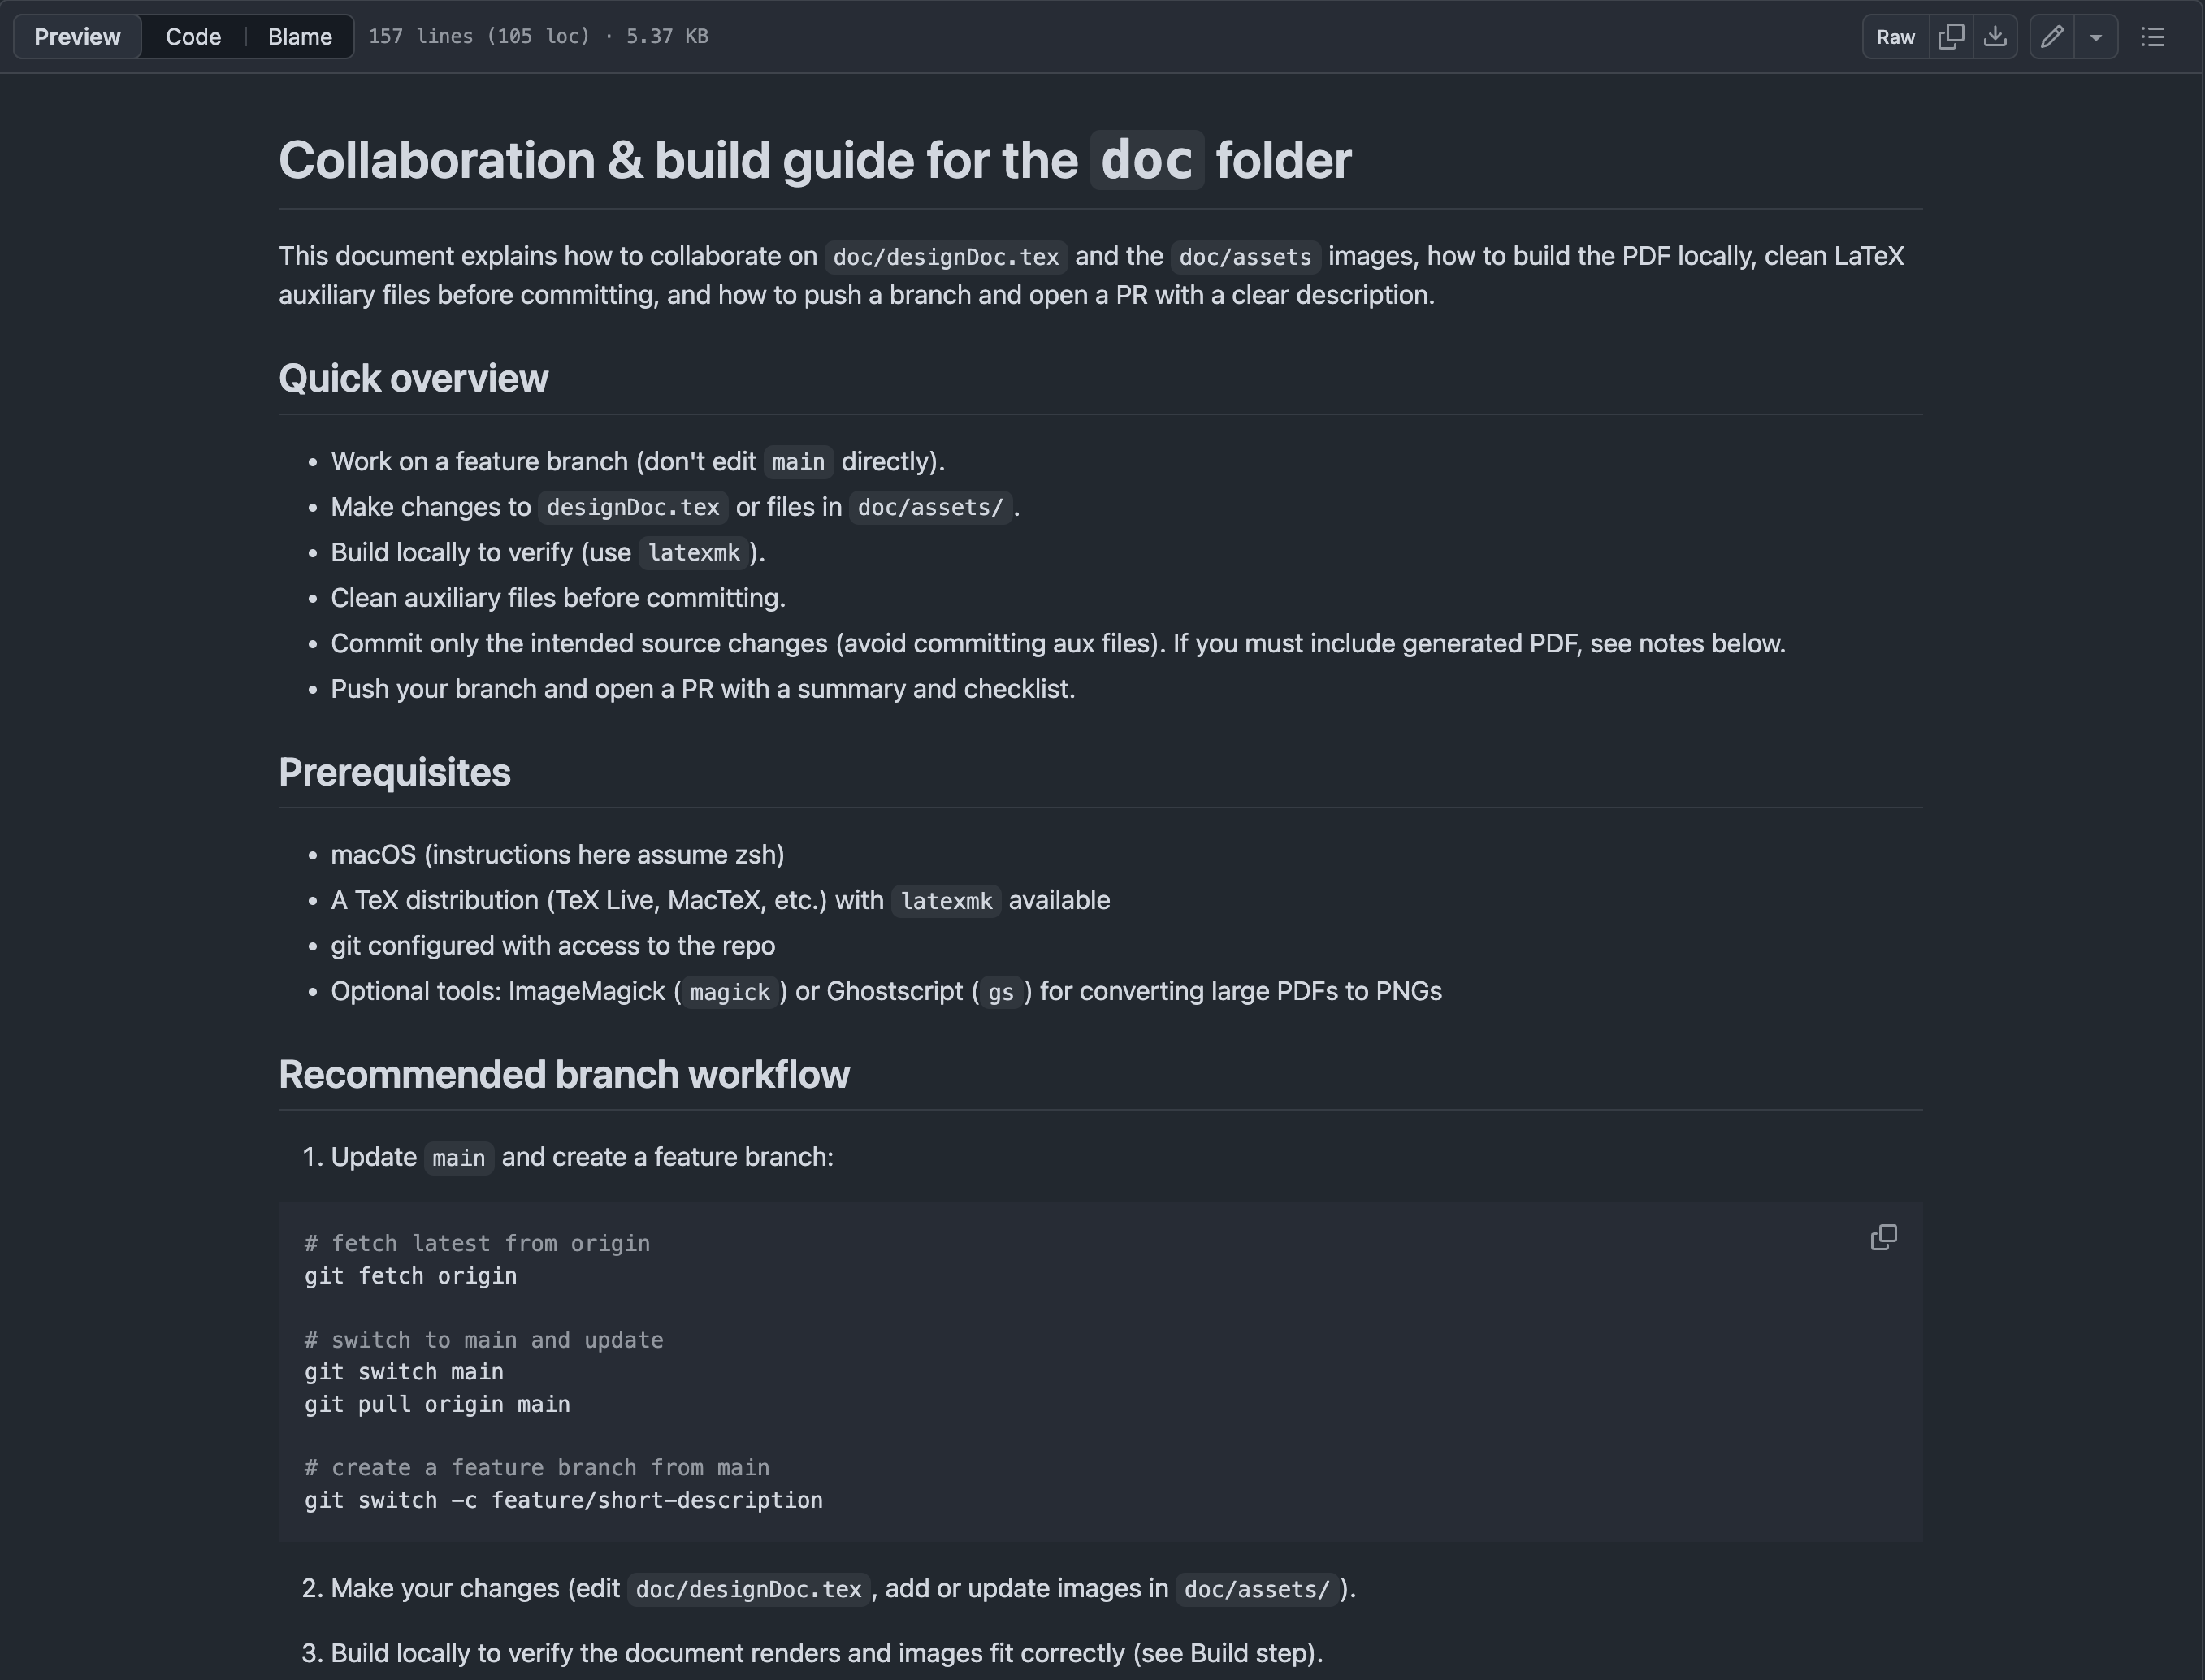
\includegraphics[width=0.95\textwidth]{assets/pm_doc_readme_overview.png}
    \caption{Repository documentation showing the team's collaboration and build workflow for the report folder.}
    \label{fig:pm-doc-readme-overview}
\end{figure}

Figure~\ref{fig:pm-doc-readme-overview} shows the team's documented workflow for working on the report. The guide instructs contributors to use feature branches, update \texttt{designDoc.tex} or files in \texttt{doc/assets/}, build locally with \texttt{latexmk}, clean auxiliary files, and open pull requests with summaries and checklists.

The workflow also supported review and accountability. Pull requests were expected to include a clear summary and checklist so reviewers could understand the purpose of the change, confirm that the correct files were updated, and verify that the document or code still worked as expected.

\begin{figure}[H]
    \centering
    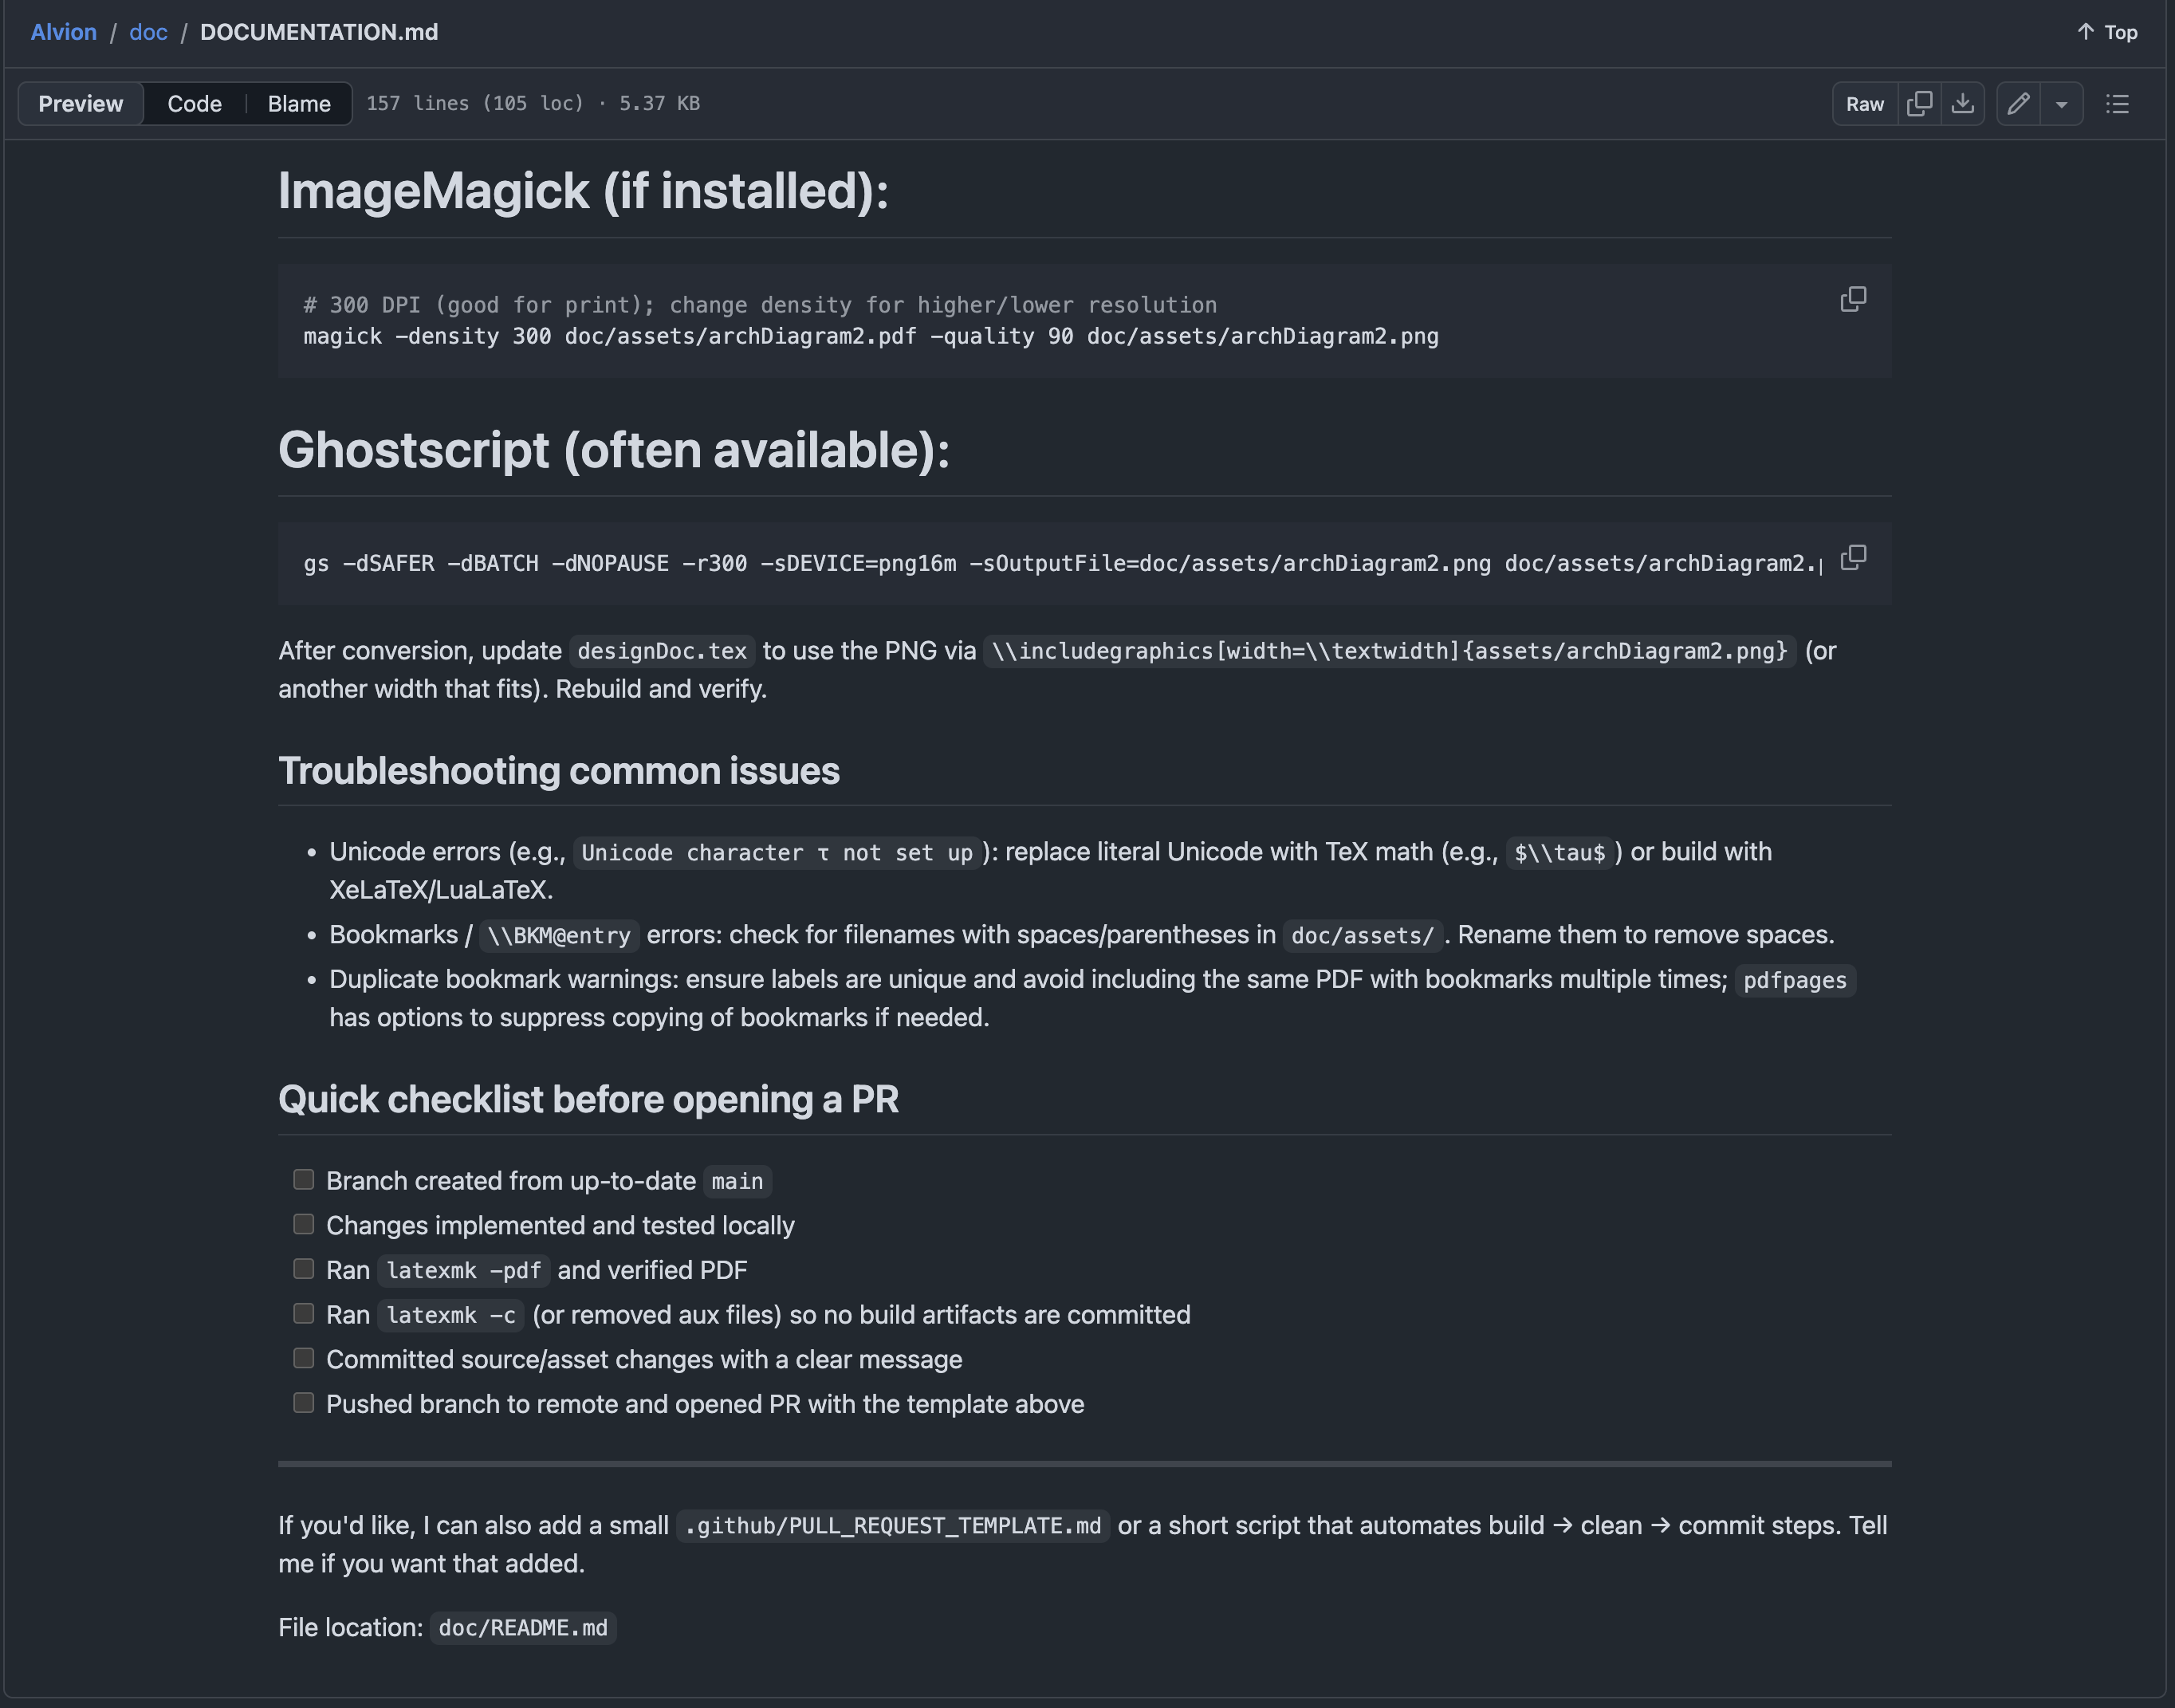
\includegraphics[width=0.95\textwidth]{assets/pm_doc_readme_checklist.png}
    \caption{Repository documentation showing the checklist used before opening a pull request.}
    \label{fig:pm-doc-readme-checklist}
\end{figure}

Figure~\ref{fig:pm-doc-readme-checklist} shows the checklist used before opening a pull request. The checklist required contributors to branch from an up-to-date main branch, test changes locally, run the LaTeX build, clean auxiliary files, commit source or asset changes with a clear message, and push the branch before opening a pull request.

\subsection*{PM.3 GitHub Issue Tracking Evidence}

GitHub Issues were used as a primary task management tool throughout the ALVION project. The issue tracker allowed the team to create work items, categorize them with labels, associate them with contributors, track discussion, and close tasks after completion. This gave the team a visible record of planned work, active work, completed work, bugs, documentation tasks, testing tasks, and feature development.

\begin{figure}[H]
    \centering
    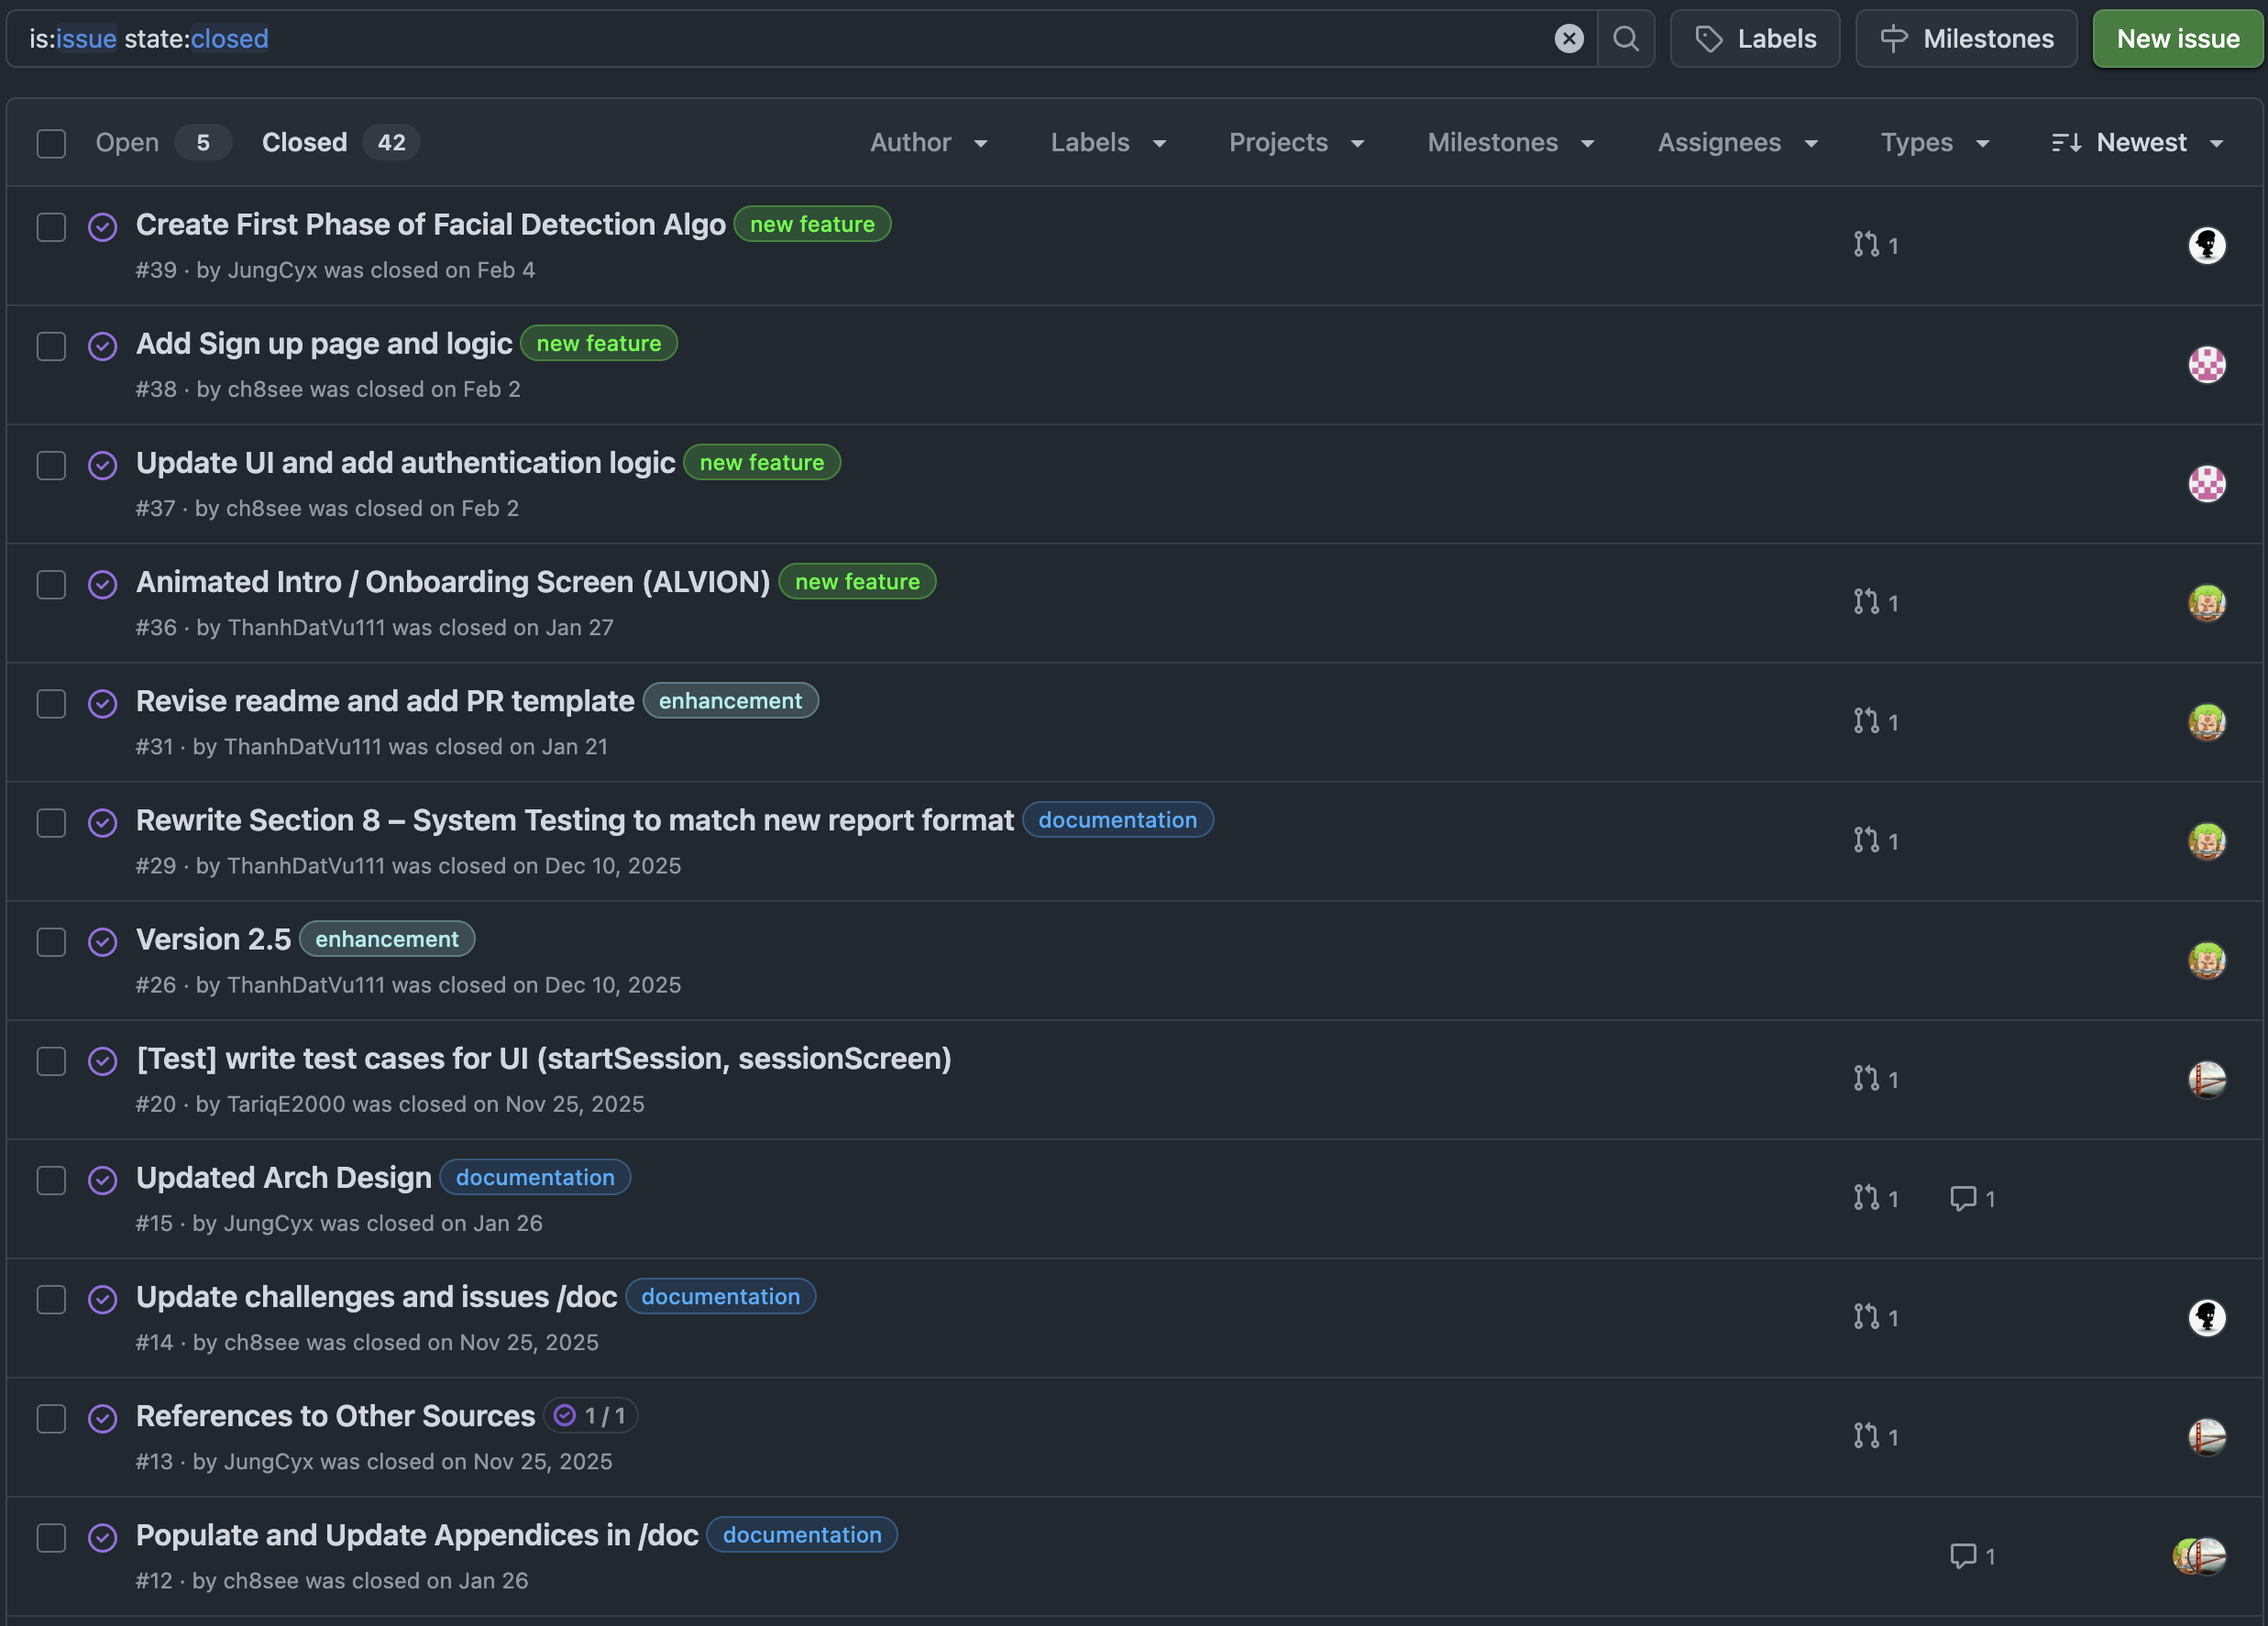
\includegraphics[width=0.98\textwidth]{assets/pm_issues_overview.png}
    \caption{GitHub closed issue overview showing 42 closed issues, 5 open issues, labels, authors, dates, and task activity across the project.}
    \label{fig:pm-issues-overview}
\end{figure}

Figure~\ref{fig:pm-issues-overview} shows the repository's closed issue tracker. The screenshot includes issue labels such as \textit{new feature}, \textit{enhancement}, and \textit{documentation}, along with issue authors, close dates, comments, and linked development activity. This demonstrates that the team tracked work items in GitHub rather than relying only on informal communication.

\begin{figure}[H]
    \centering
    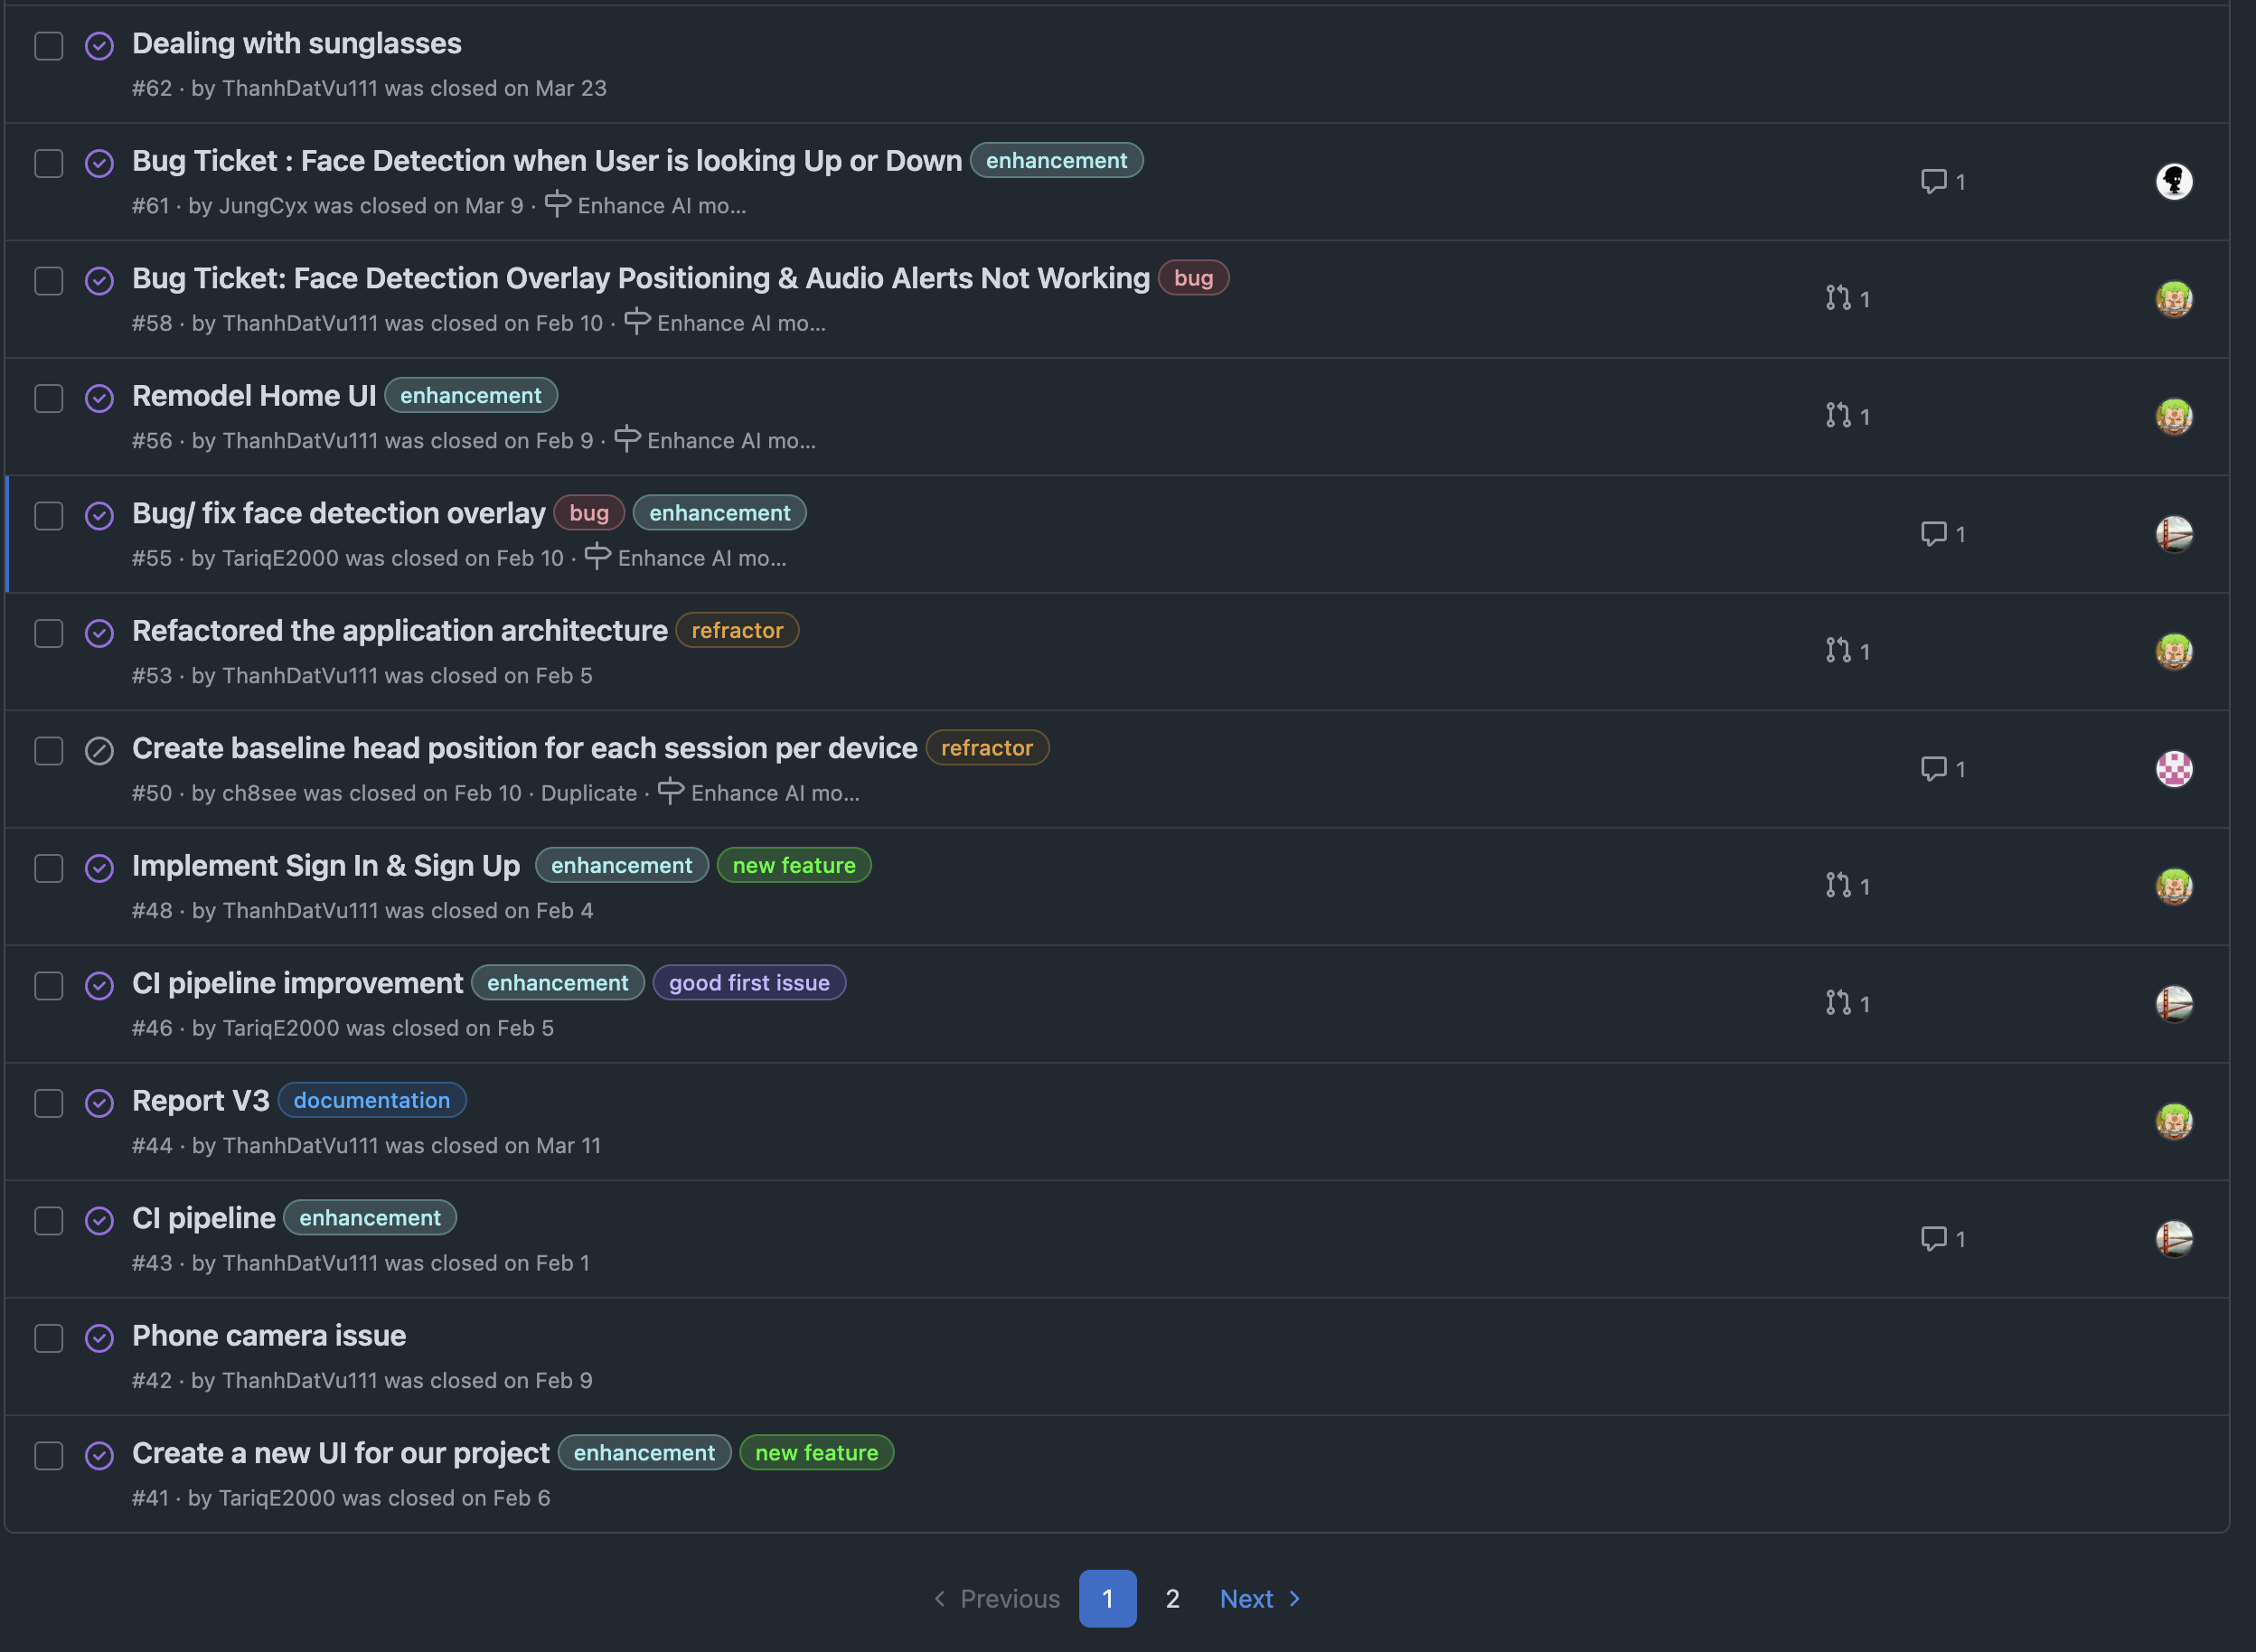
\includegraphics[width=0.98\textwidth]{assets/pm_issues_implementation.png}
    \caption{GitHub issues showing implementation, bug-fixing, refactoring, authentication, CI pipeline, and UI development tasks.}
    \label{fig:pm-issues-implementation}
\end{figure}

Figure~\ref{fig:pm-issues-implementation} shows issue records from active implementation phases. These issues include face detection bug fixes, application architecture refactoring, sign-in and sign-up implementation, CI pipeline improvements, camera issues, and UI redesign. This evidence shows that the team tracked technical implementation work, defects, and process improvements through GitHub Issues.

\begin{figure}[H]
    \centering
    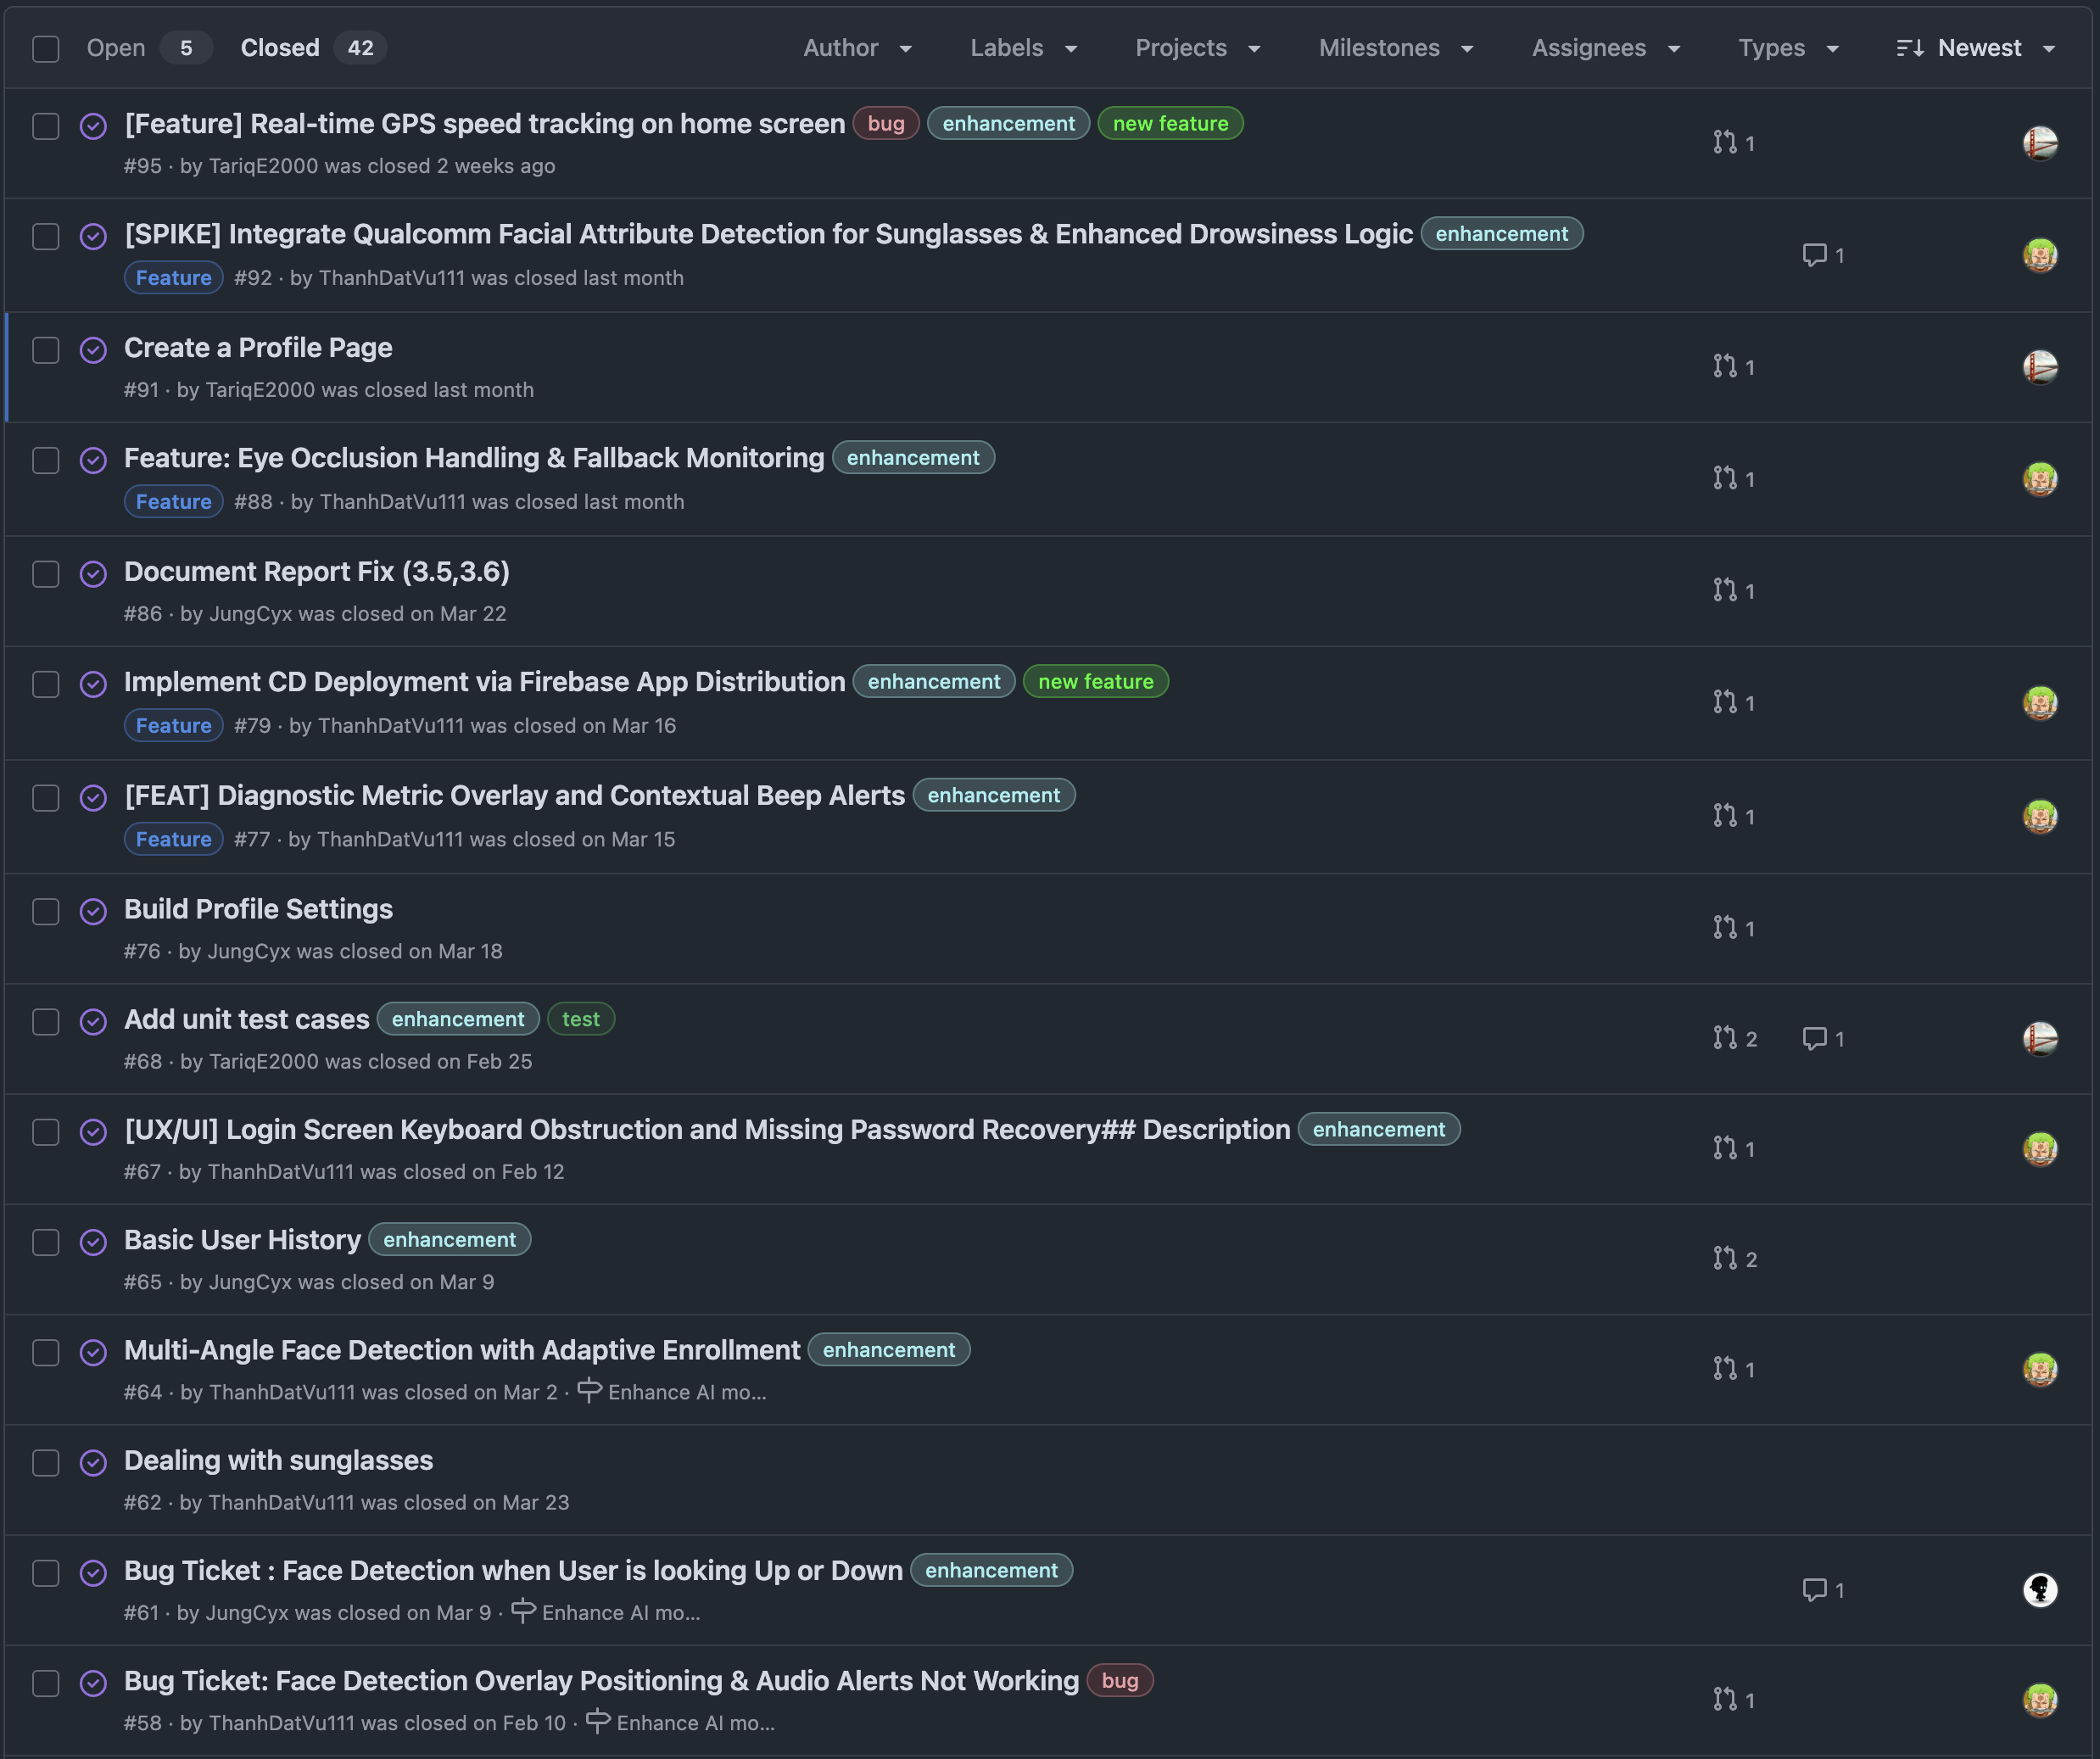
\includegraphics[width=0.98\textwidth]{assets/pm_issues_late_stage.png}
    \caption{GitHub issues showing later-stage feature work, deployment work, profile work, testing work, and AI robustness improvements.}
    \label{fig:pm-issues-late-stage}
\end{figure}

Figure~\ref{fig:pm-issues-late-stage} shows later-stage issue tracking. The issues include real-time GPS speed tracking, Qualcomm facial attribute detection, profile page creation, eye occlusion handling, Firebase App Distribution deployment, diagnostic overlays, profile settings, unit test cases, user history, and multi-angle face detection. This demonstrates that the team continued using project management records through the later phases of development.

\begin{figure}[H]
    \centering
    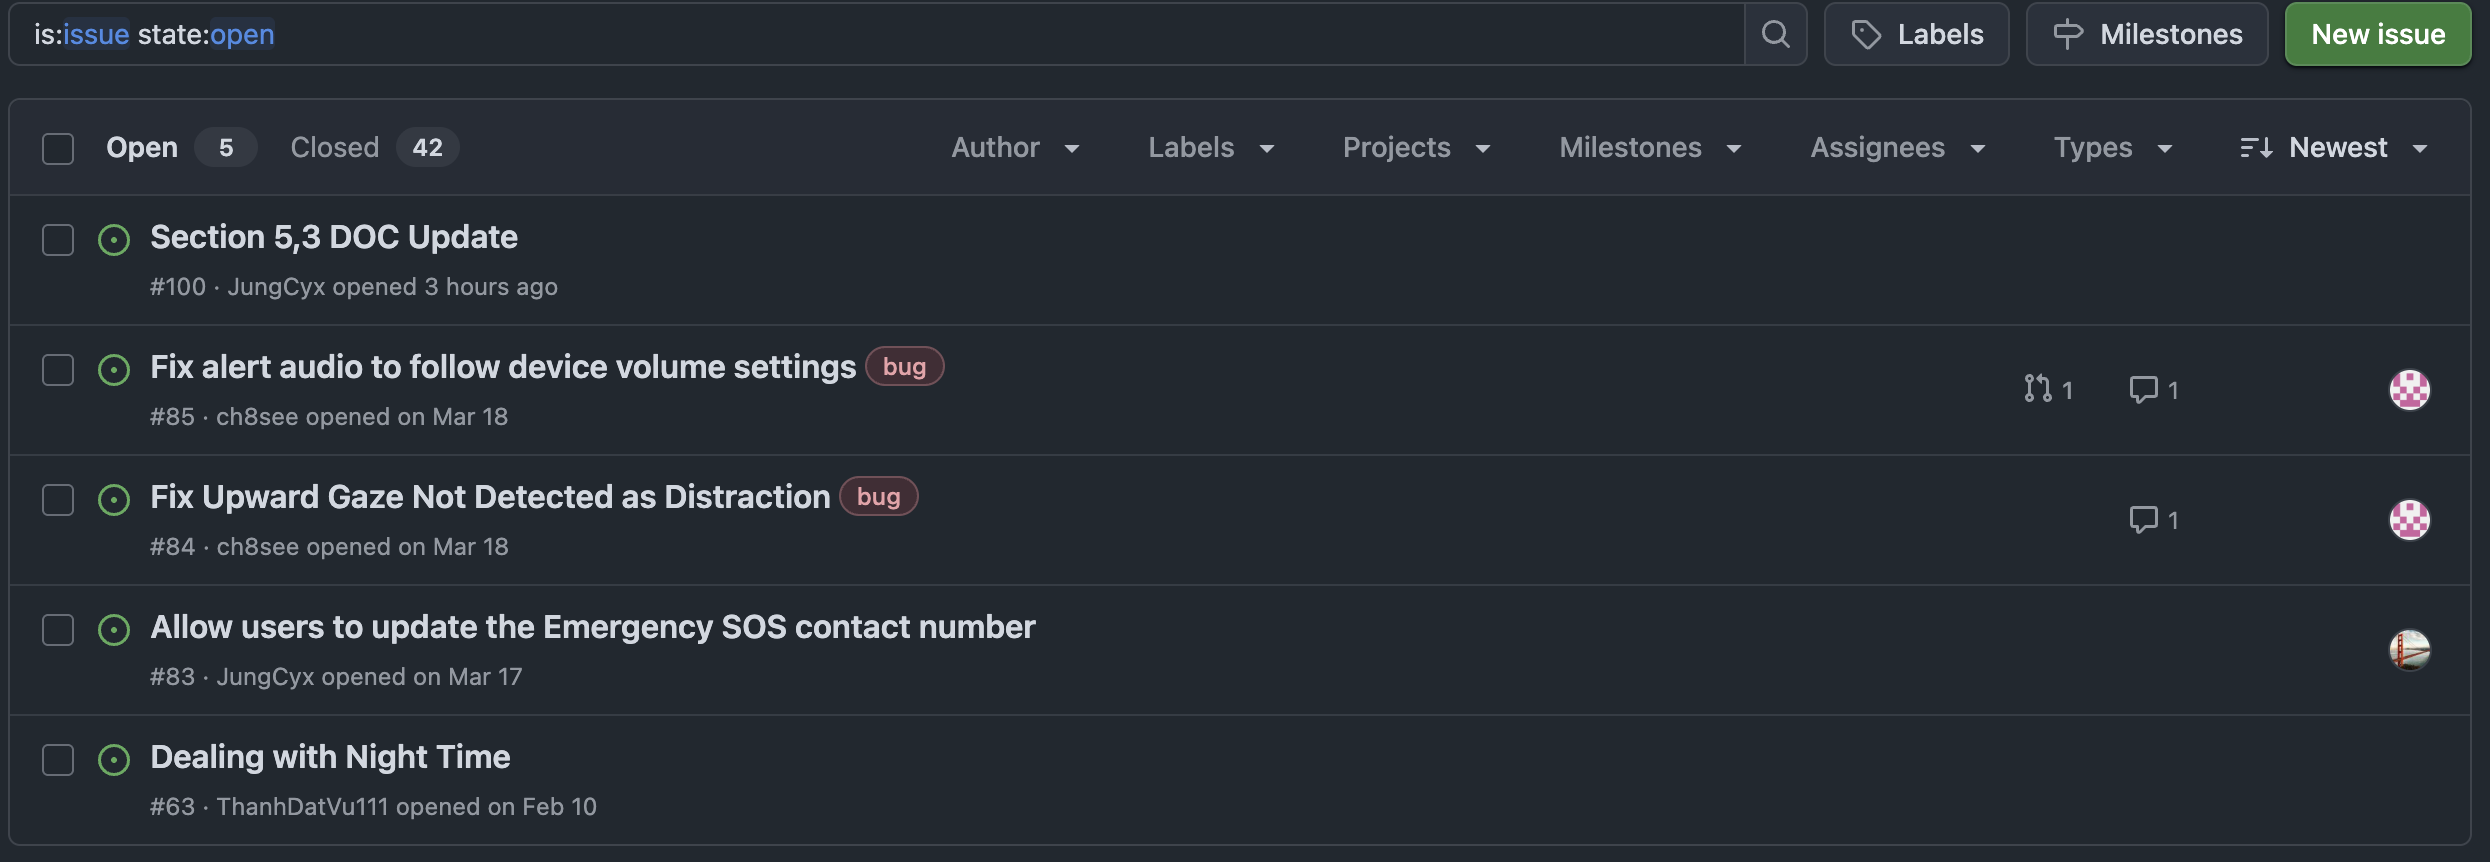
\includegraphics[width=0.98\textwidth]{assets/pm_issues_open_items.png}
    \caption{GitHub open issue list showing remaining work items and unresolved bugs tracked by the team.}
    \label{fig:pm-issues-open-items}
\end{figure}

Figure~\ref{fig:pm-issues-open-items} shows the open issue list near the end of the project. These open issues include remaining documentation updates, audio behavior fixes, upward gaze detection, emergency contact updates, and night-time handling. This shows that the team tracked both completed tasks and remaining work, which is important for project status visibility.

Overall, the issue tracker provides evidence of project management across multiple categories of work. The team used issues to organize feature development, bug resolution, documentation, testing, refactoring, CI/CD improvements, and unresolved follow-up tasks throughout the project lifecycle.

\subsection*{PM.4 Task Allocation and Individual Contributions}

The repository history provides evidence of individual task allocation through pull request authorship, issue authorship, branch names, review requests, issue references, and merged implementation records. While some tasks were discussed and completed collaboratively, the GitHub records show clear ownership patterns for major work areas.

\begin{longtable}{|p{3cm}|p{5cm}|p{6cm}|}
\hline
\textbf{Team Member} & \textbf{Primary Contribution Areas} & \textbf{Repository Evidence} \\
\hline
\endfirsthead

\hline
\textbf{Team Member} & \textbf{Primary Contribution Areas} & \textbf{Repository Evidence} \\
\hline
\endhead

Thanh Dat Vu &
Onboarding UI, Firebase authentication, app architecture refactoring, Home dashboard redesign, calibration and diagnostic overlay improvements, CI/CD deployment, final UI redesign, and report updates. &
Pull requests show work on the onboarding intro screen, Firebase Auth, architecture refactor, Home UI redesign, diagnostic overlay/contextual alerts, Firebase App Distribution deployment, revised UI, and Report V4 documentation. \\
\hline

Tariq Elamin &
Repository setup, early UI updates, UI testing, vibration alerts, face-detection unit testing, profile page work, and GPS speed tracking. &
Pull requests show work on branch protection, icon/color updates, UI test cases, vibration feature, face analyzer unit-test refactor, additional face-detection unit tests, profile page creation, and live GPS speed tracking. \\
\hline

Salman Shekh &
Core facial detection implementation, profile/settings features, and history-related development. &
Pull requests and issue records show work on the ML Kit facial detection pipeline, profile settings, and history/profile feature development. \\
\hline

Chase Tanner &
Contributed to end-to-end testing, ML Kit model development including calibration, and bug discovery. Additionally handled audio alert fixes, issue tracking, documentation-related tasks, and review participation. &
Repository records show ML Kit model development and calibration, bug discovery, audio fixes, documentation, and participation in review/requested-review workflows. \\
\hline

\end{longtable}

\begin{figure}[H]
    \centering
    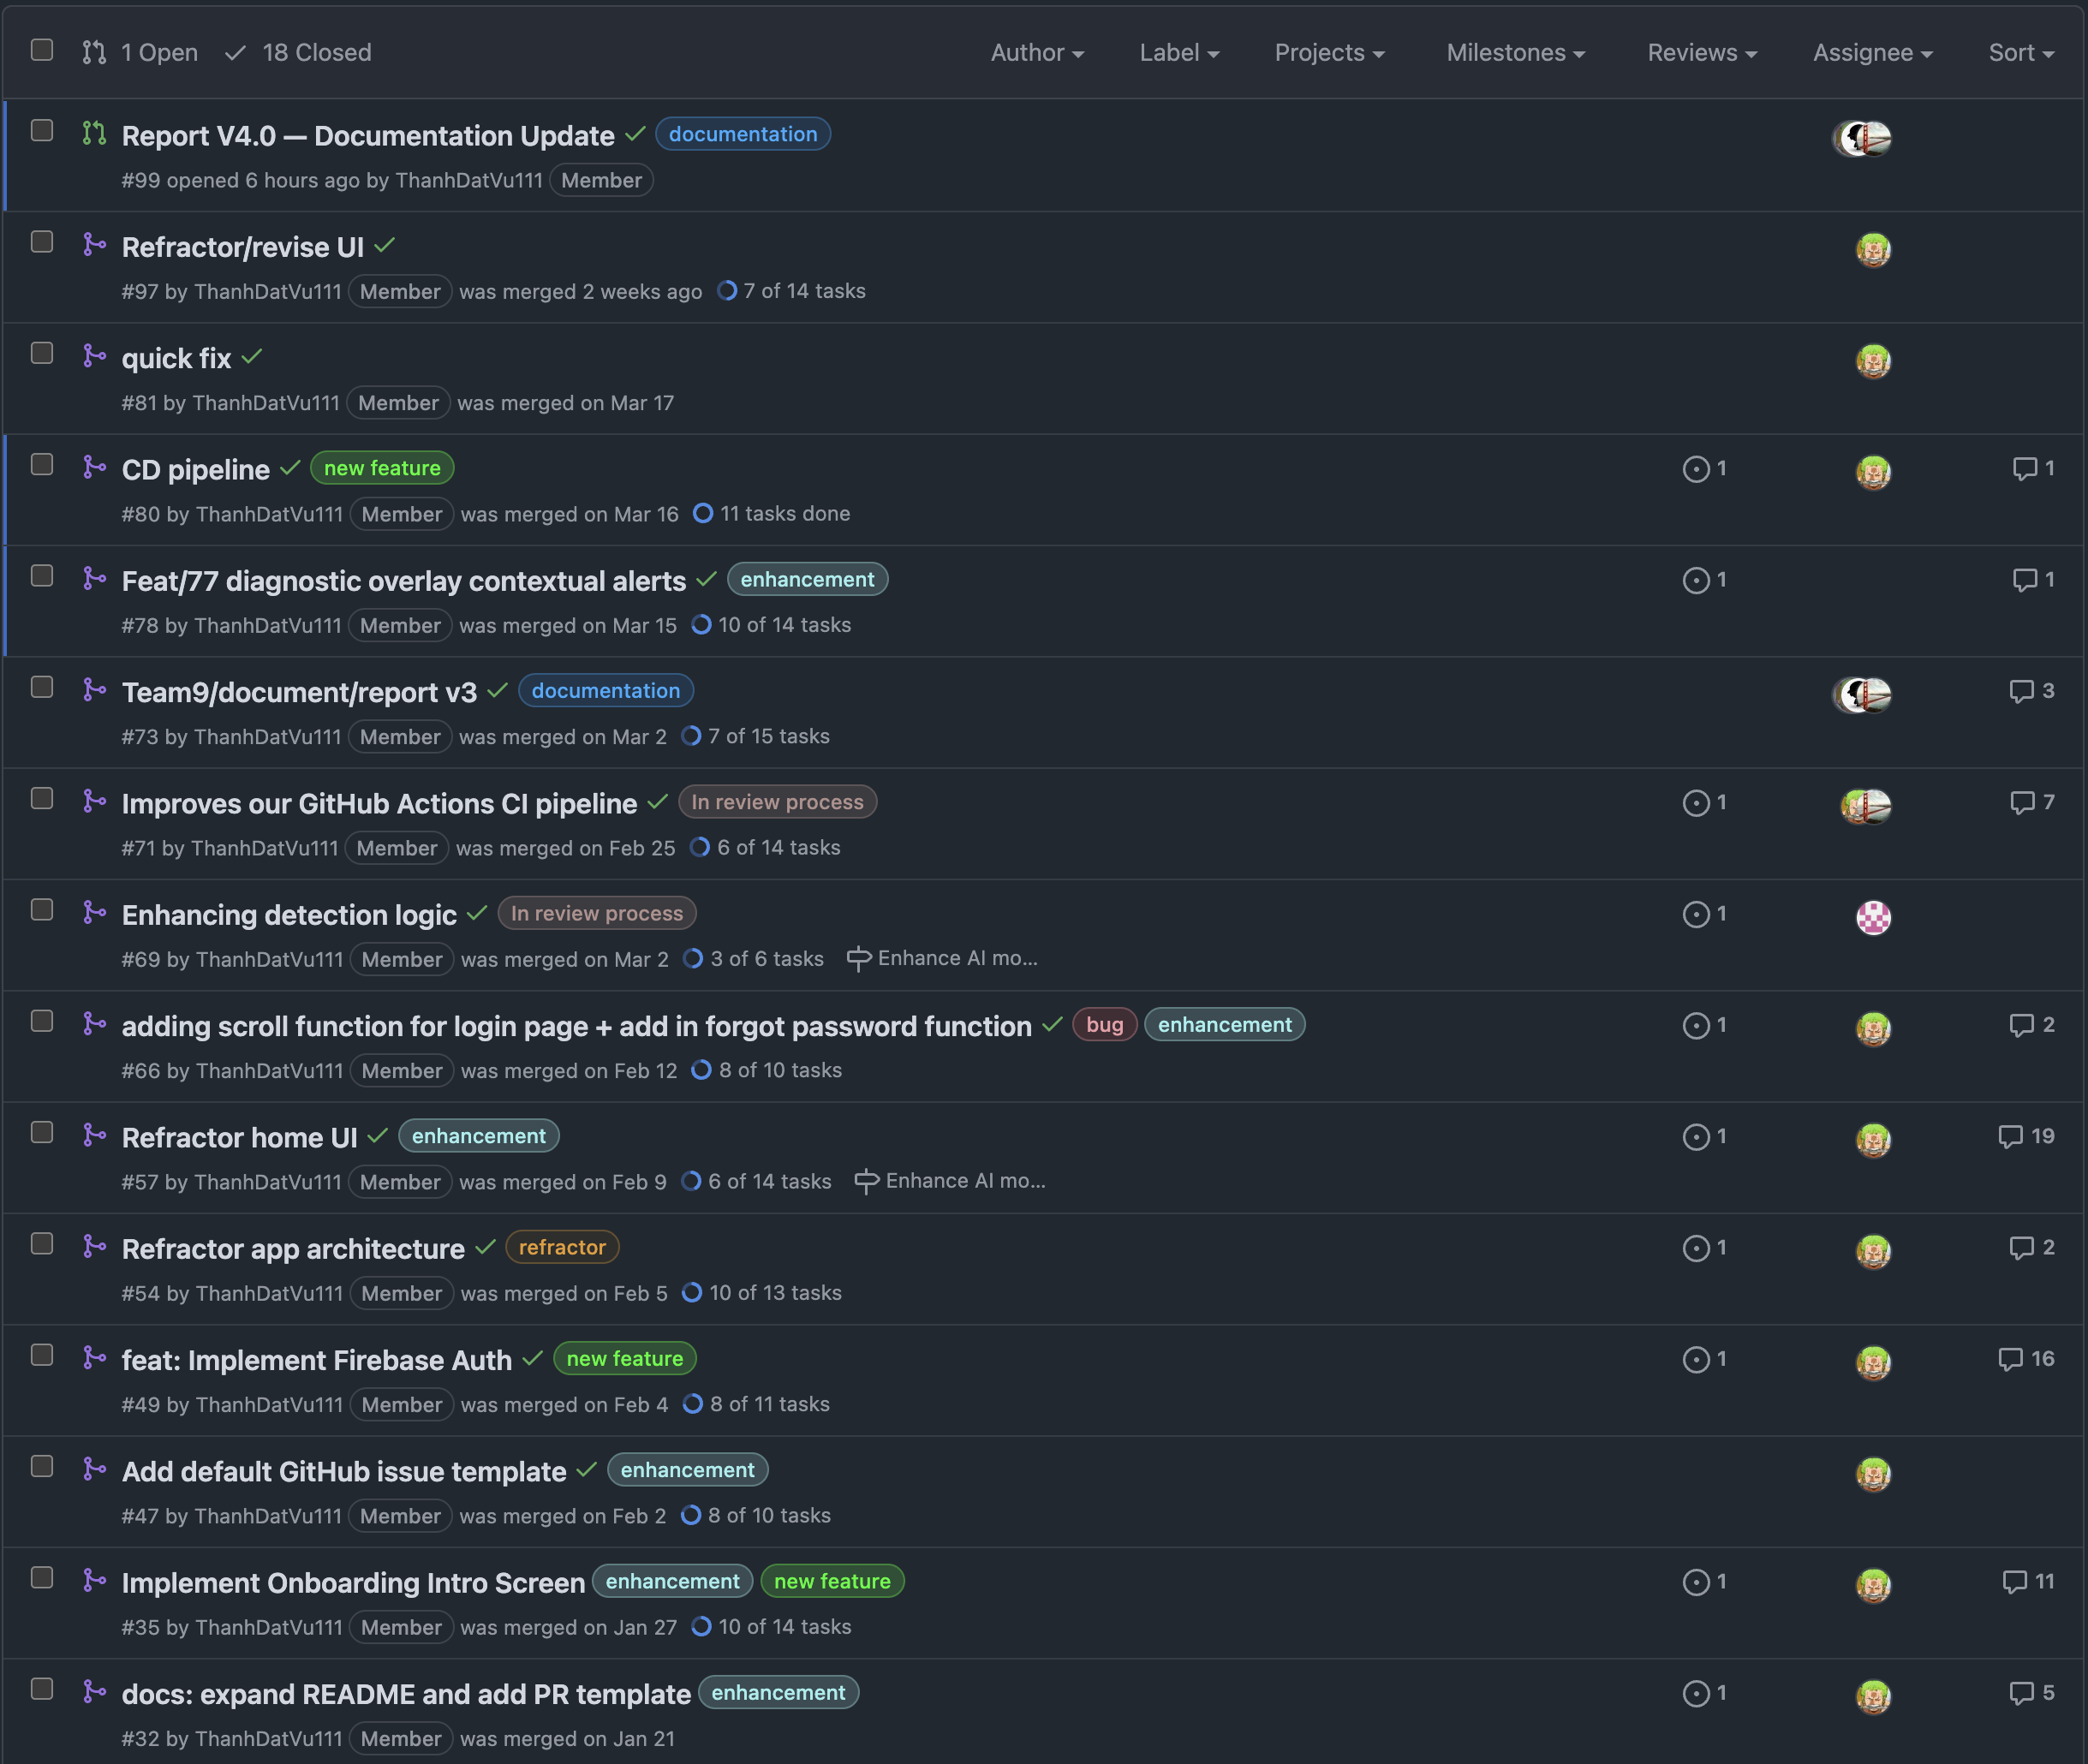
\includegraphics[width=0.98\textwidth]{assets/pm_contributions_thanh.png}
    \caption{GitHub pull request records filtered by Thanh Dat Vu, showing ownership of UI, architecture, authentication, CI/CD, and documentation work.}
    \label{fig:pm-contributions-thanh}
\end{figure}

Figure~\ref{fig:pm-contributions-thanh} shows repository records for Thanh Dat Vu's contributions. The pull request history provides evidence of ownership across major implementation and documentation areas, including onboarding, authentication, app architecture, Home UI, diagnostic overlays, deployment, and report updates.

\begin{figure}[H]
    \centering
    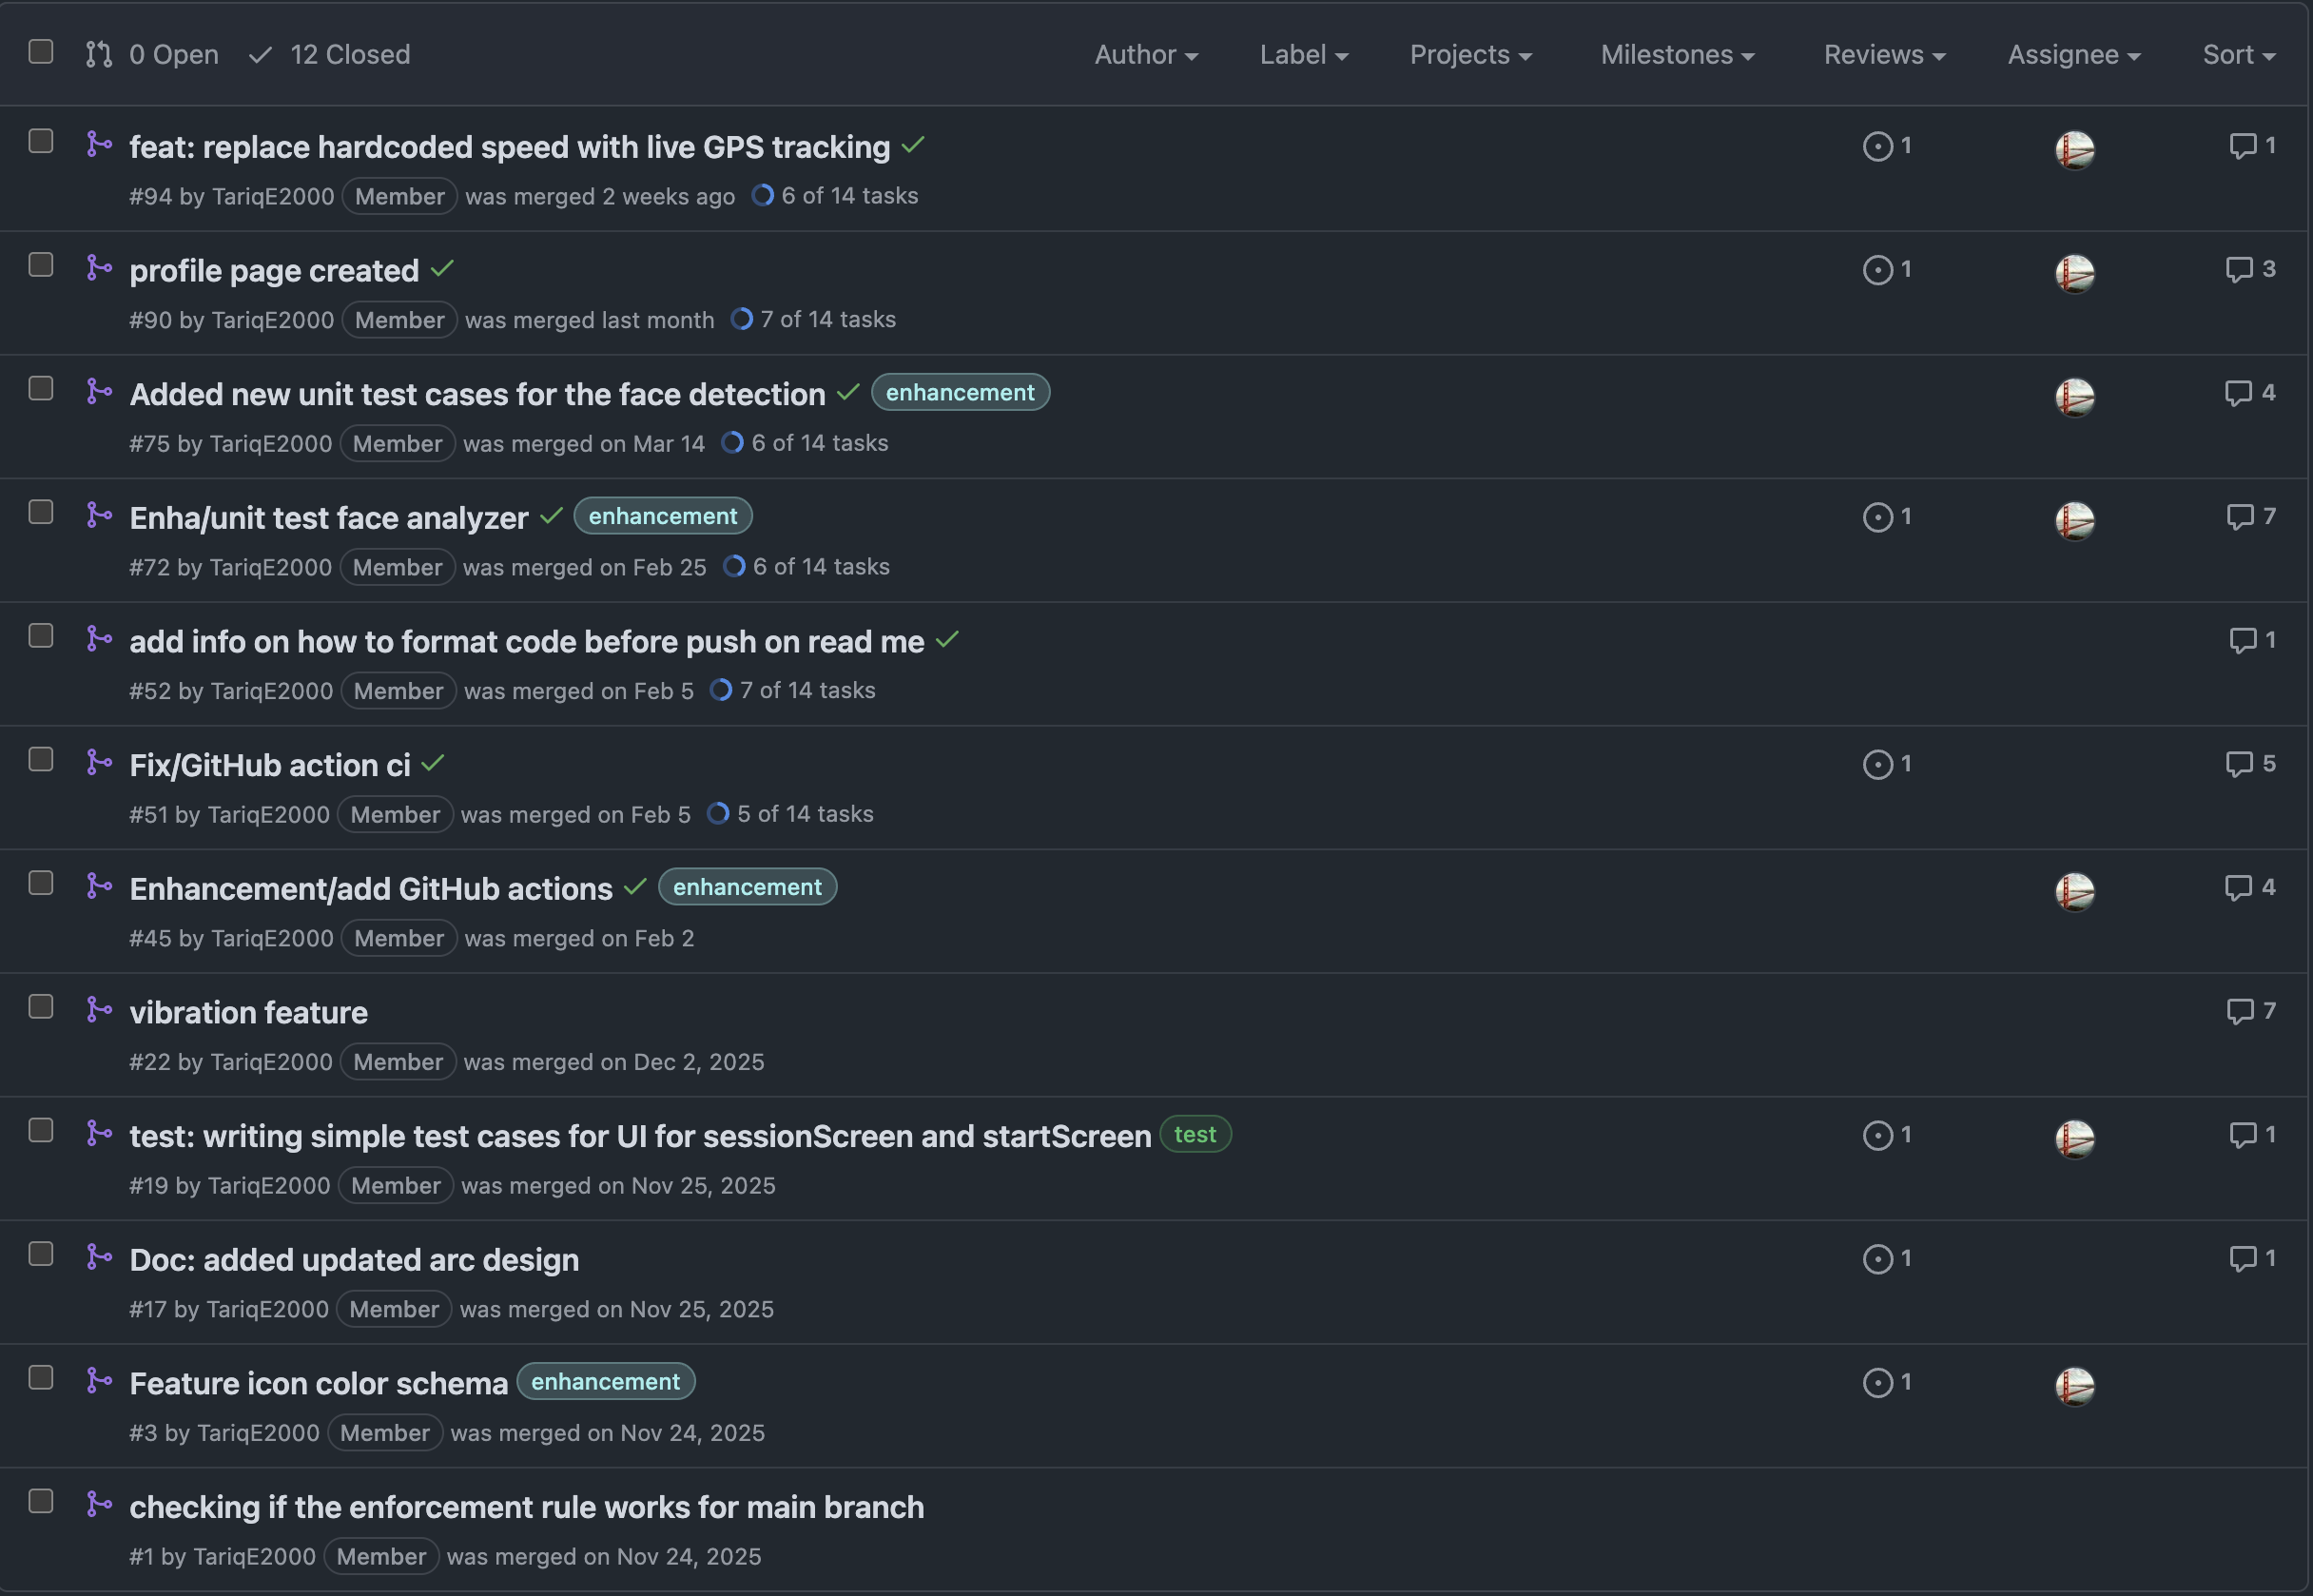
\includegraphics[width=0.98\textwidth]{assets/pm_contributions_tariq.png}
    \caption{GitHub pull request records filtered by Tariq Elamin, showing ownership of testing, profile, GPS speed tracking, alert, and repository setup work.}
    \label{fig:pm-contributions-tariq}
\end{figure}

Figure~\ref{fig:pm-contributions-tariq} shows repository records for Tariq Elamin's contributions. The pull request history provides evidence of work on early repository setup, UI updates, testing, vibration alerts, face-detection unit tests, profile page implementation, and GPS speed tracking.

\begin{figure}[H]
    \centering
    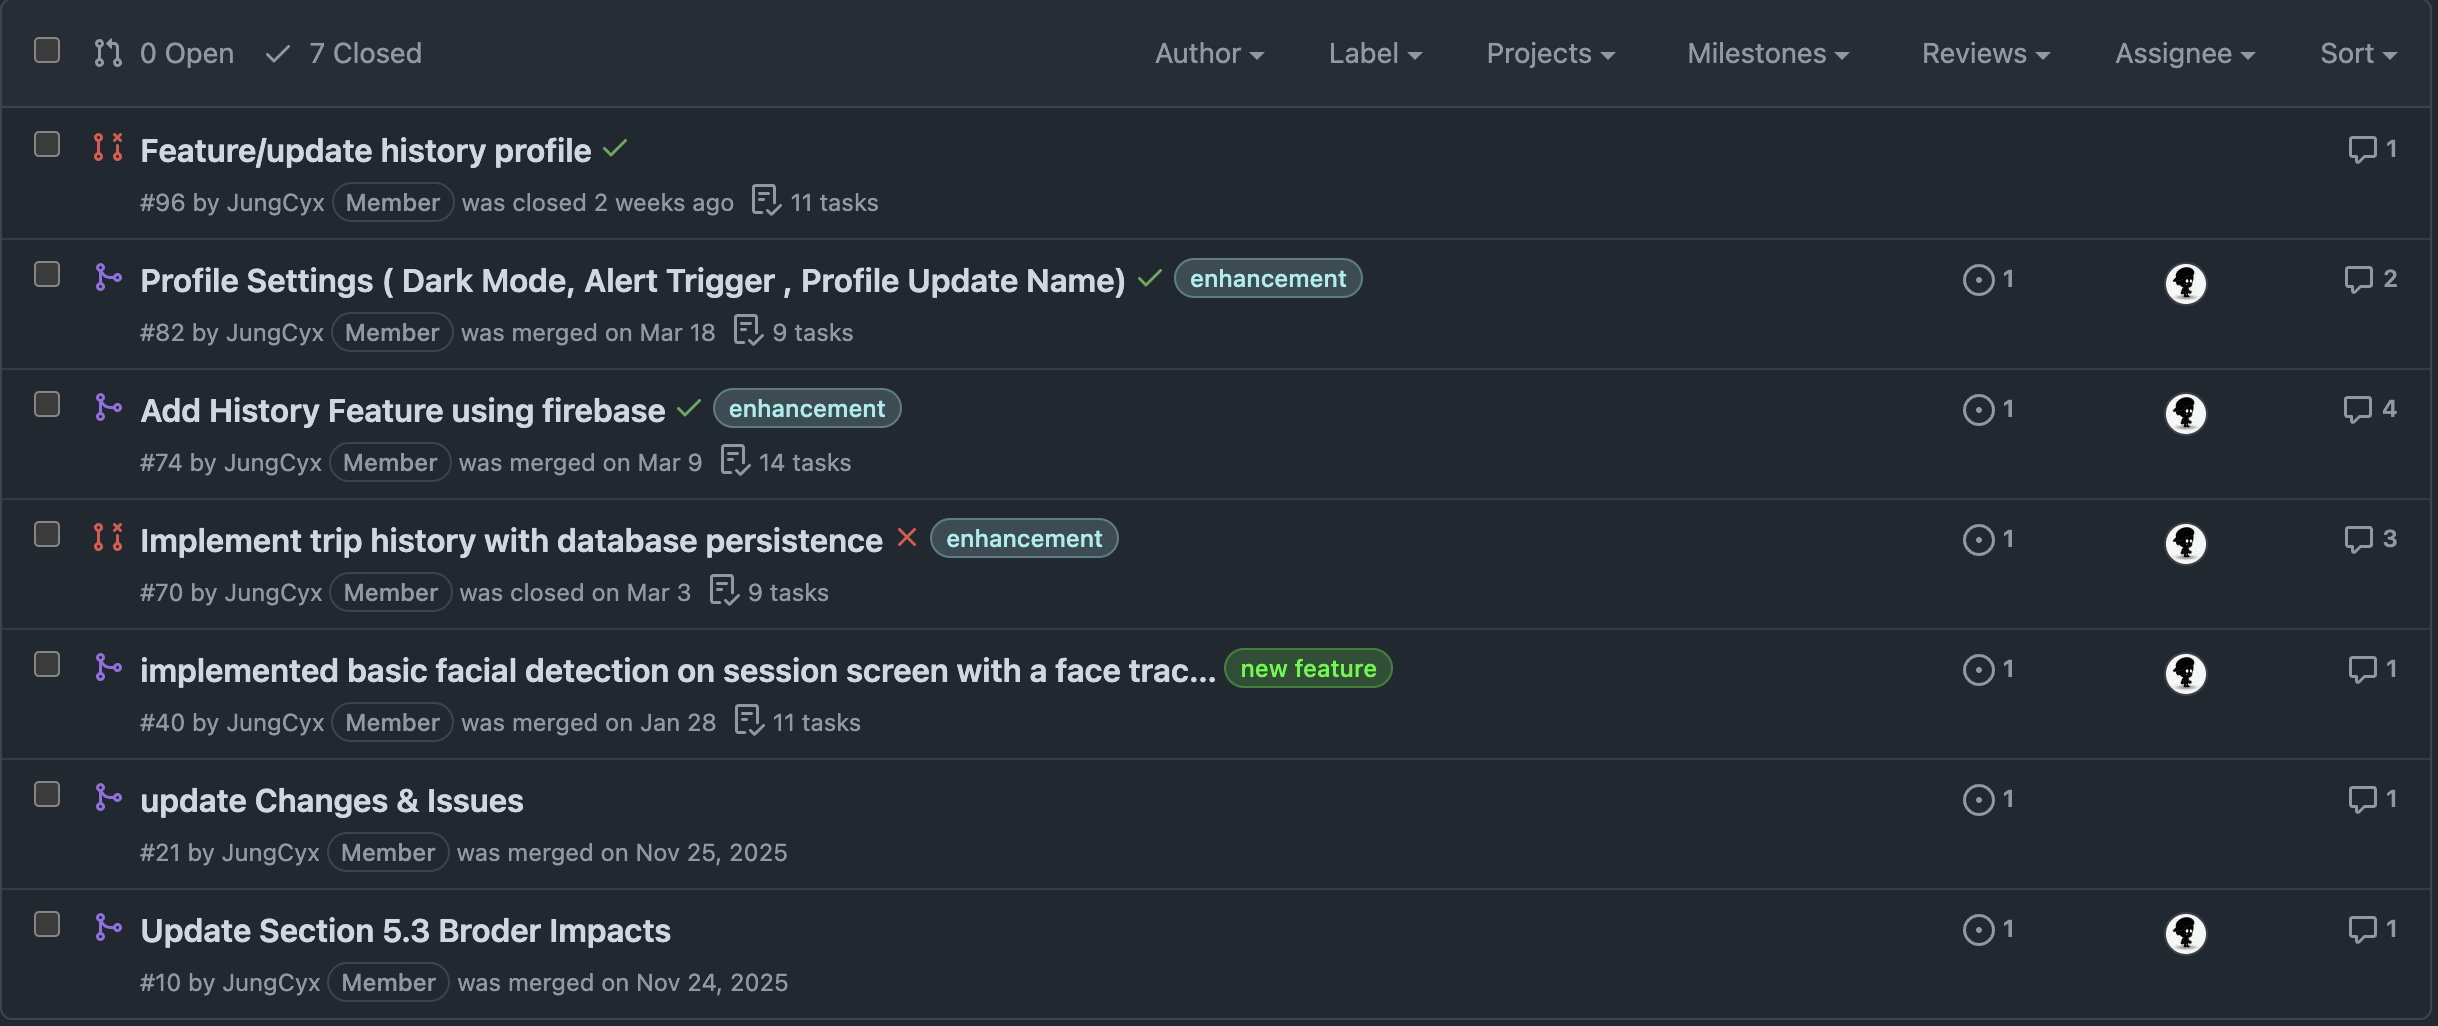
\includegraphics[width=0.98\textwidth]{assets/pm_contributions_salman.png}
    \caption{GitHub pull request records filtered by Salman Shekh, showing ownership of facial detection, profile/settings, and history-related development work.}
    \label{fig:pm-contributions-salman}
\end{figure}

Figure~\ref{fig:pm-contributions-salman} shows repository records for Salman Shekh's contributions. The records provide evidence of work related to the facial detection MVP, profile settings, and history/profile feature development.

\begin{figure}[H]
    \centering
    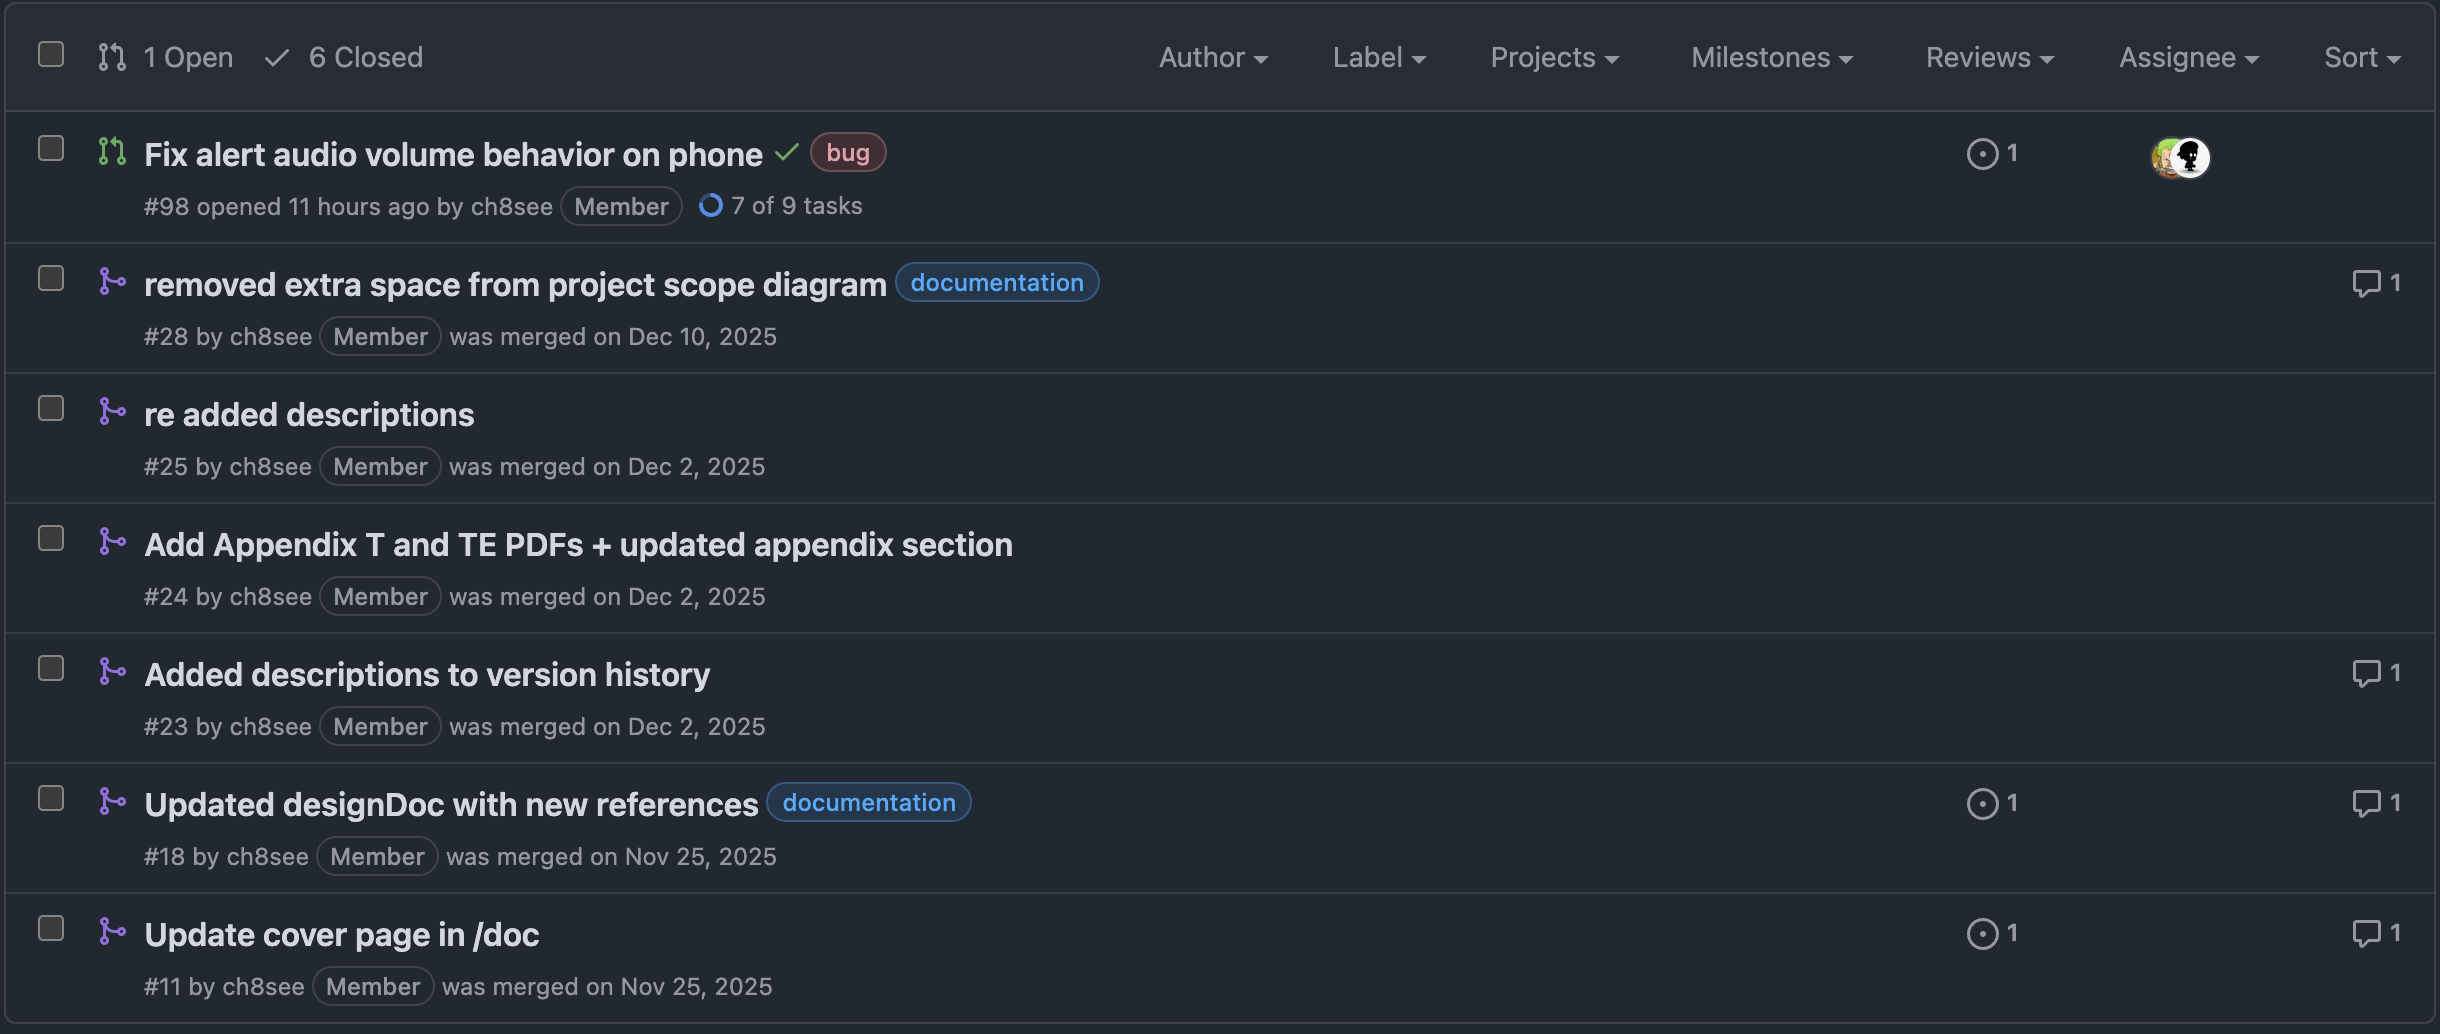
\includegraphics[width=0.98\textwidth]{assets/pm_contributions_chase.png}
    \caption{GitHub records filtered by Chase Tanner, showing issue ownership, audio-related fixes, documentation work, and review participation.}
    \label{fig:pm-contributions-chase}
\end{figure}

Figure~\ref{fig:pm-contributions-chase} shows repository records for Chase Tanner's contributions. The records provide evidence of issue ownership, audio-related bug tracking or fixes, documentation-related work, and participation in the team's GitHub workflow.

Overall, these contribution records show that the team divided work across members and maintained visible ownership of tasks. The records support both task allocation and individual contribution tracking, which are required project management artifacts.

\subsection*{PM.5 Pull Request Review and Branch Workflow}

GitHub Pull Requests were used to manage review and merging of project changes. Contributors worked on separate branches and opened pull requests to describe the purpose of their changes, identify the type of work completed, document testing performed, and provide checklists before merging. This helped the team review changes before they entered the main branch.

Pull requests also provided accountability because each record showed the author, branch name, merge status, changed files, commits, checks, and testing notes. This made it possible to trace implementation work back to contributors and verify that major changes were reviewed before becoming part of the main project.

\begin{figure}[H]
    \centering
    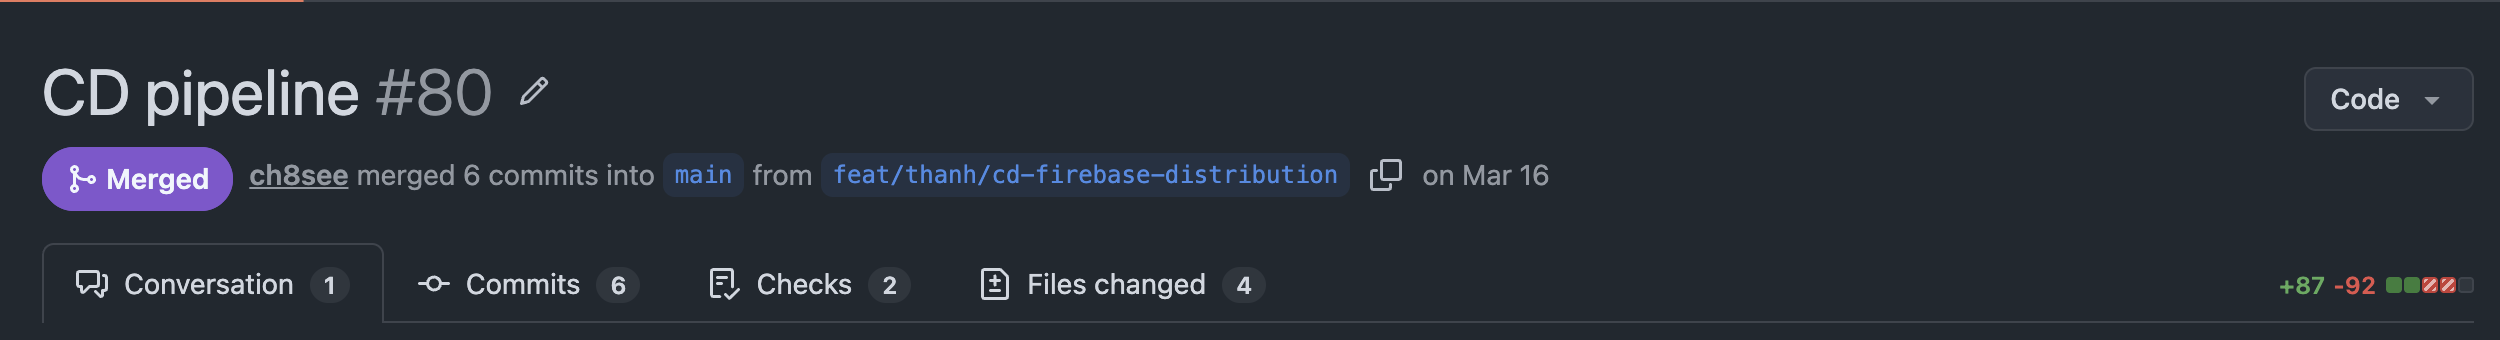
\includegraphics[width=0.98\textwidth]{assets/pm_pr_merged_workflow.png}
    \caption{Merged GitHub pull request showing branch-based development, merge status, commits, checks, and changed files.}
    \label{fig:pm-pr-merged-workflow}
\end{figure}

Figure~\ref{fig:pm-pr-merged-workflow} shows PR \#80 for the CD pipeline. The record shows that the work was completed on a separate feature branch, \texttt{feat/thanh/cd-firebase-distribution}, and then merged into \texttt{main}. It also shows the number of commits, checks, changed files, and code additions/deletions. This supports the team's use of branch-based development and pull request review instead of direct untracked changes to the main branch.

\begin{figure}[H]
    \centering
    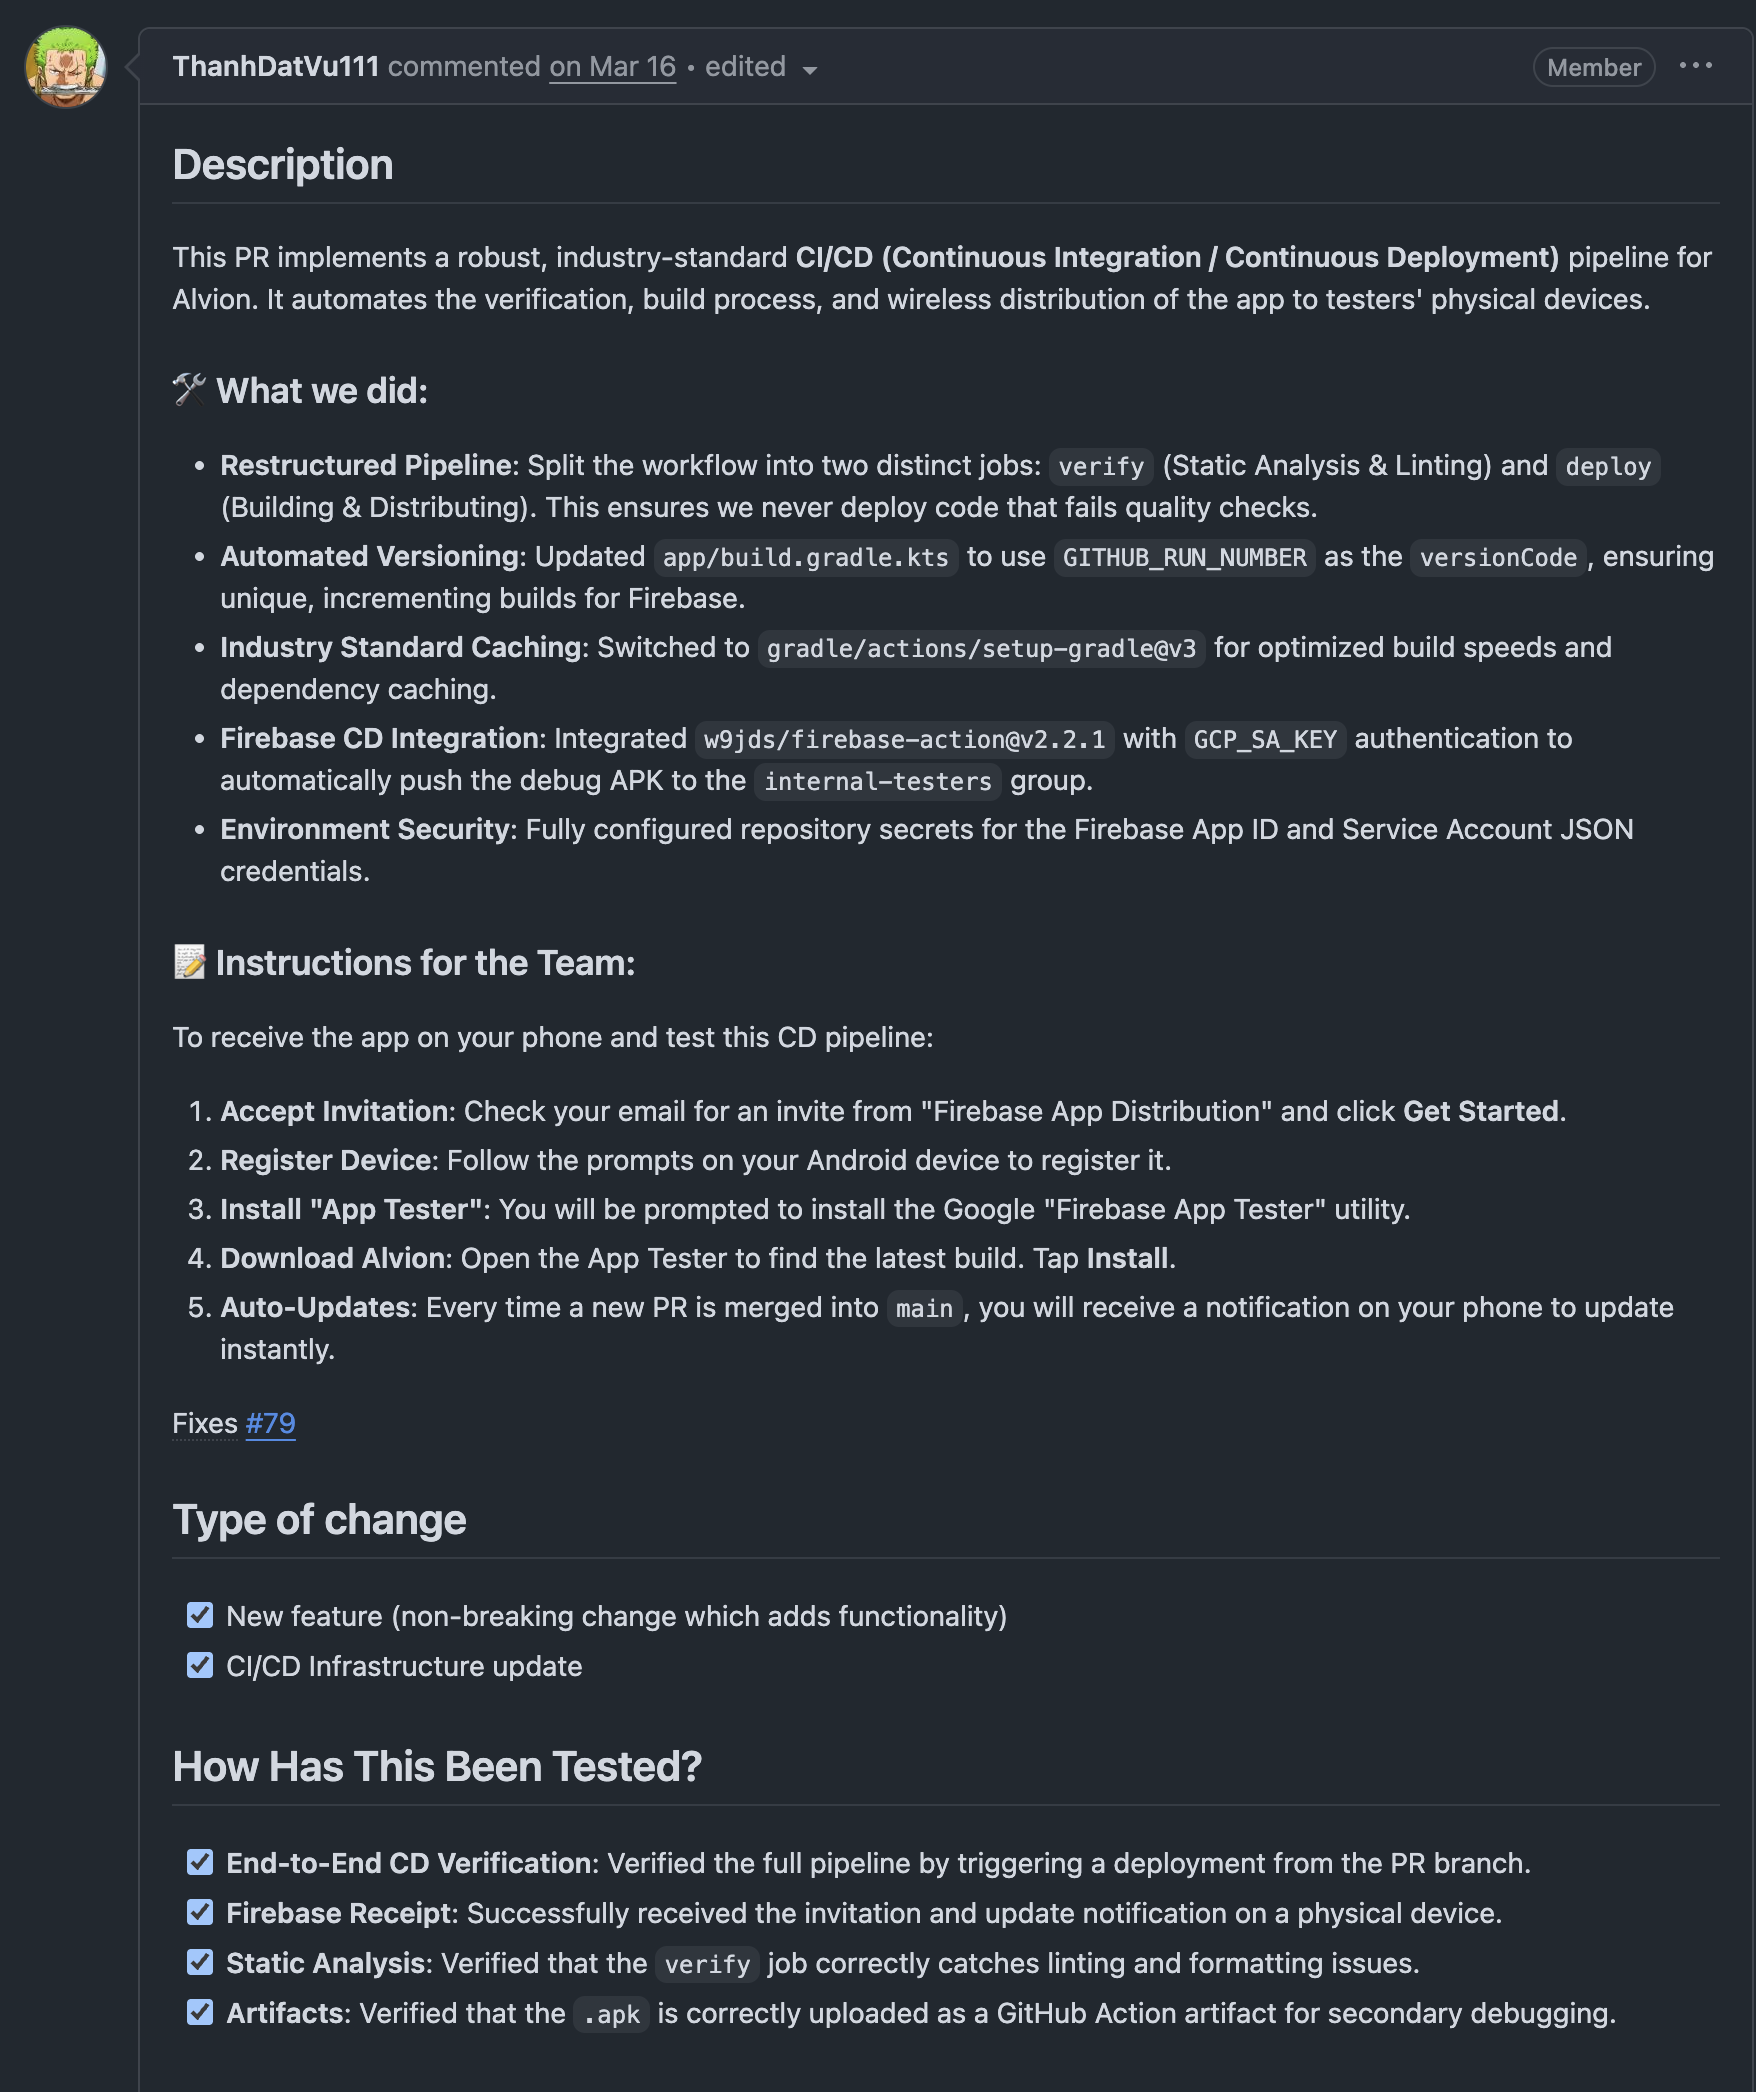
\includegraphics[width=0.98\textwidth]{assets/pm_pr_checklist_testing.png}
    \caption{Pull request description showing summary, implementation details, type of change, and testing evidence.}
    \label{fig:pm-pr-checklist-testing}
\end{figure}

Figure~\ref{fig:pm-pr-checklist-testing} shows the pull request body for the CD pipeline work. The PR description explains what was implemented, including the verification job, deployment job, automated versioning, dependency caching, Firebase App Distribution integration, and repository secret configuration. The testing section records end-to-end CD verification, Firebase receipt, static analysis checks, and artifact upload verification.

\begin{figure}[H]
    \centering
    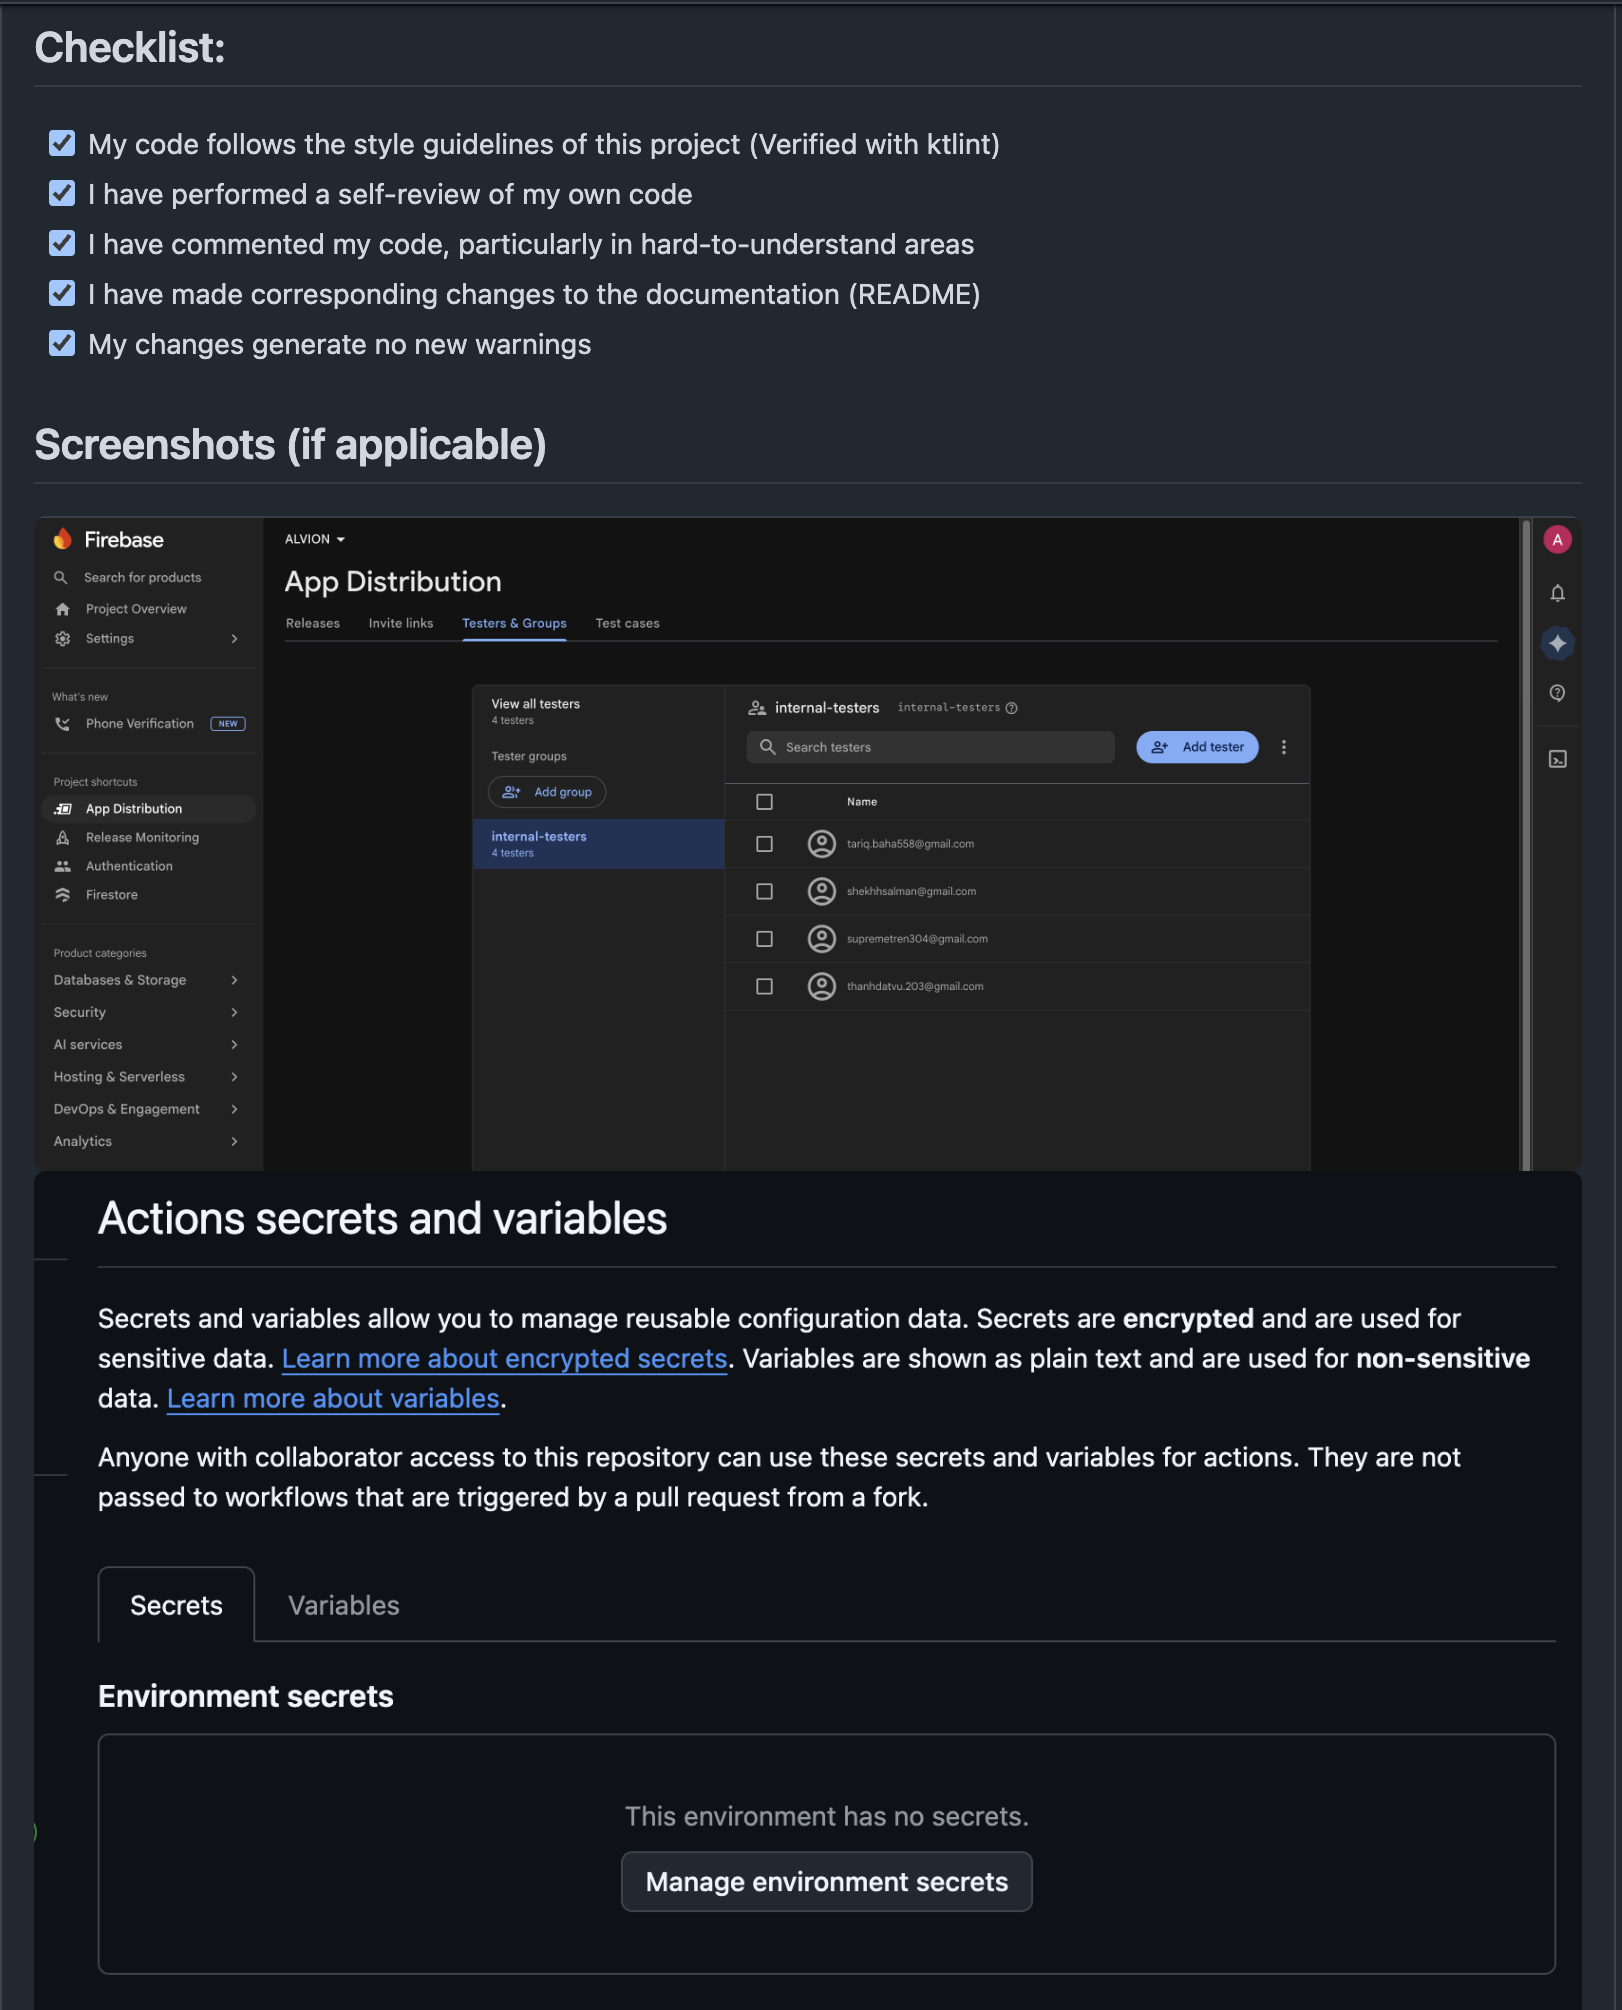
\includegraphics[width=0.98\textwidth]{assets/pm_pr_cd_evidence.png}
    \caption{Pull request checklist and deployment evidence showing completed review checklist items and Firebase App Distribution setup.}
    \label{fig:pm-pr-cd-evidence}
\end{figure}

Figure~\ref{fig:pm-pr-cd-evidence} shows the checklist and deployment evidence associated with the CD pipeline pull request. The checklist records that the contributor followed style guidelines, performed a self-review, commented the code, updated documentation, and confirmed no new warnings. The Firebase App Distribution screenshot provides additional evidence that the deployment workflow supported tester distribution.

Overall, the pull request records show that the team used a branch-based workflow with review checkpoints, testing notes, and documented verification before merging. This helped manage technical risk, improve code quality, document decisions, and maintain a clear history of project contributions.

\subsection*{PM.6 CI/CD and Testing Management Evidence}

The ALVION team used GitHub Actions to support automated quality control during development. The CI/CD workflow helped verify that changes could be checked, built, and prepared for deployment before becoming part of the main project. This provided an additional project management record because workflow runs showed when automated checks were triggered, whether they passed or failed, and which changes required follow-up.

The team also used CI/CD improvements as tracked project tasks. GitHub Issues and Pull Requests included work related to CI pipeline setup, linting, build verification, unit testing, artifact generation, and Firebase App Distribution. These records show that testing and deployment were managed as part of the project process rather than treated as informal final steps.

\begin{figure}[H]
    \centering
    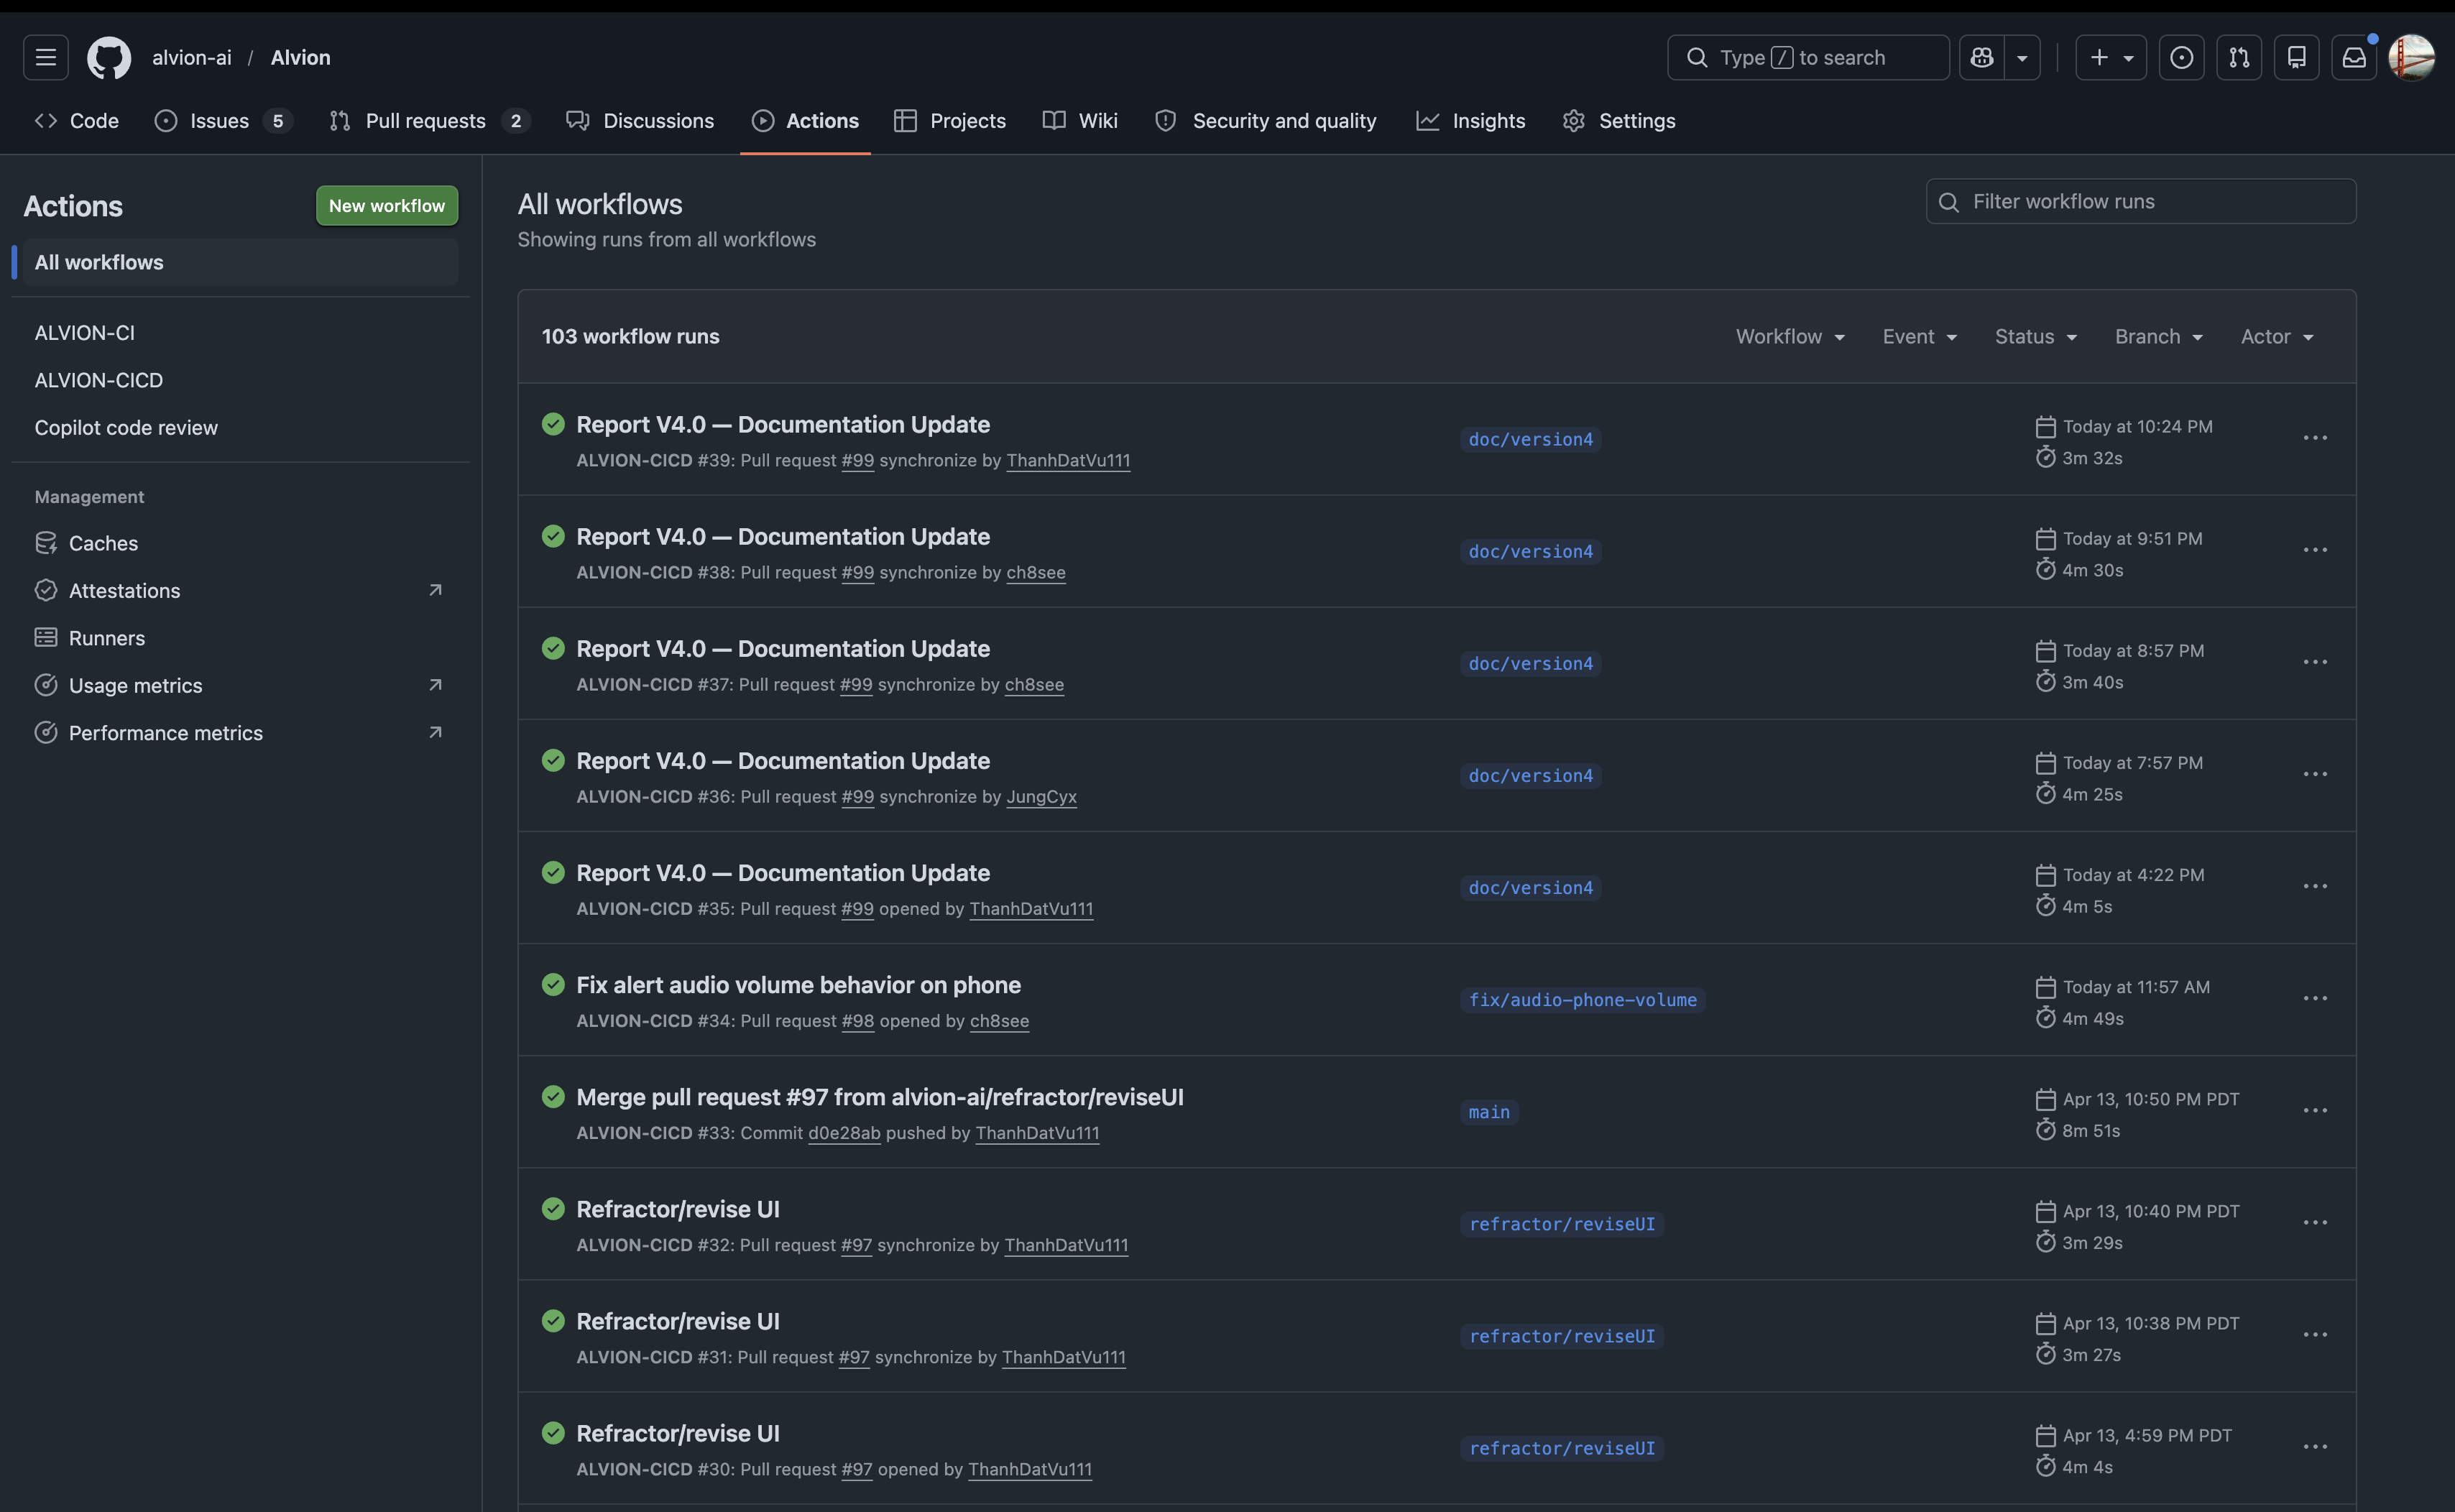
\includegraphics[width=0.98\textwidth]{assets/pm_actions_successful_run.png}
    \caption{GitHub Actions workflow list showing automated CI/CD runs used to verify project changes.}
    \label{fig:pm-actions-workflow-runs}
\end{figure}

Figure~\ref{fig:pm-actions-workflow-runs} shows the GitHub Actions workflow history for the repository. The workflow list provides evidence that automated checks were run throughout development. This helped the team monitor build health, identify failing changes, and maintain visibility into the status of the codebase.

\begin{figure}[H]
    \centering
    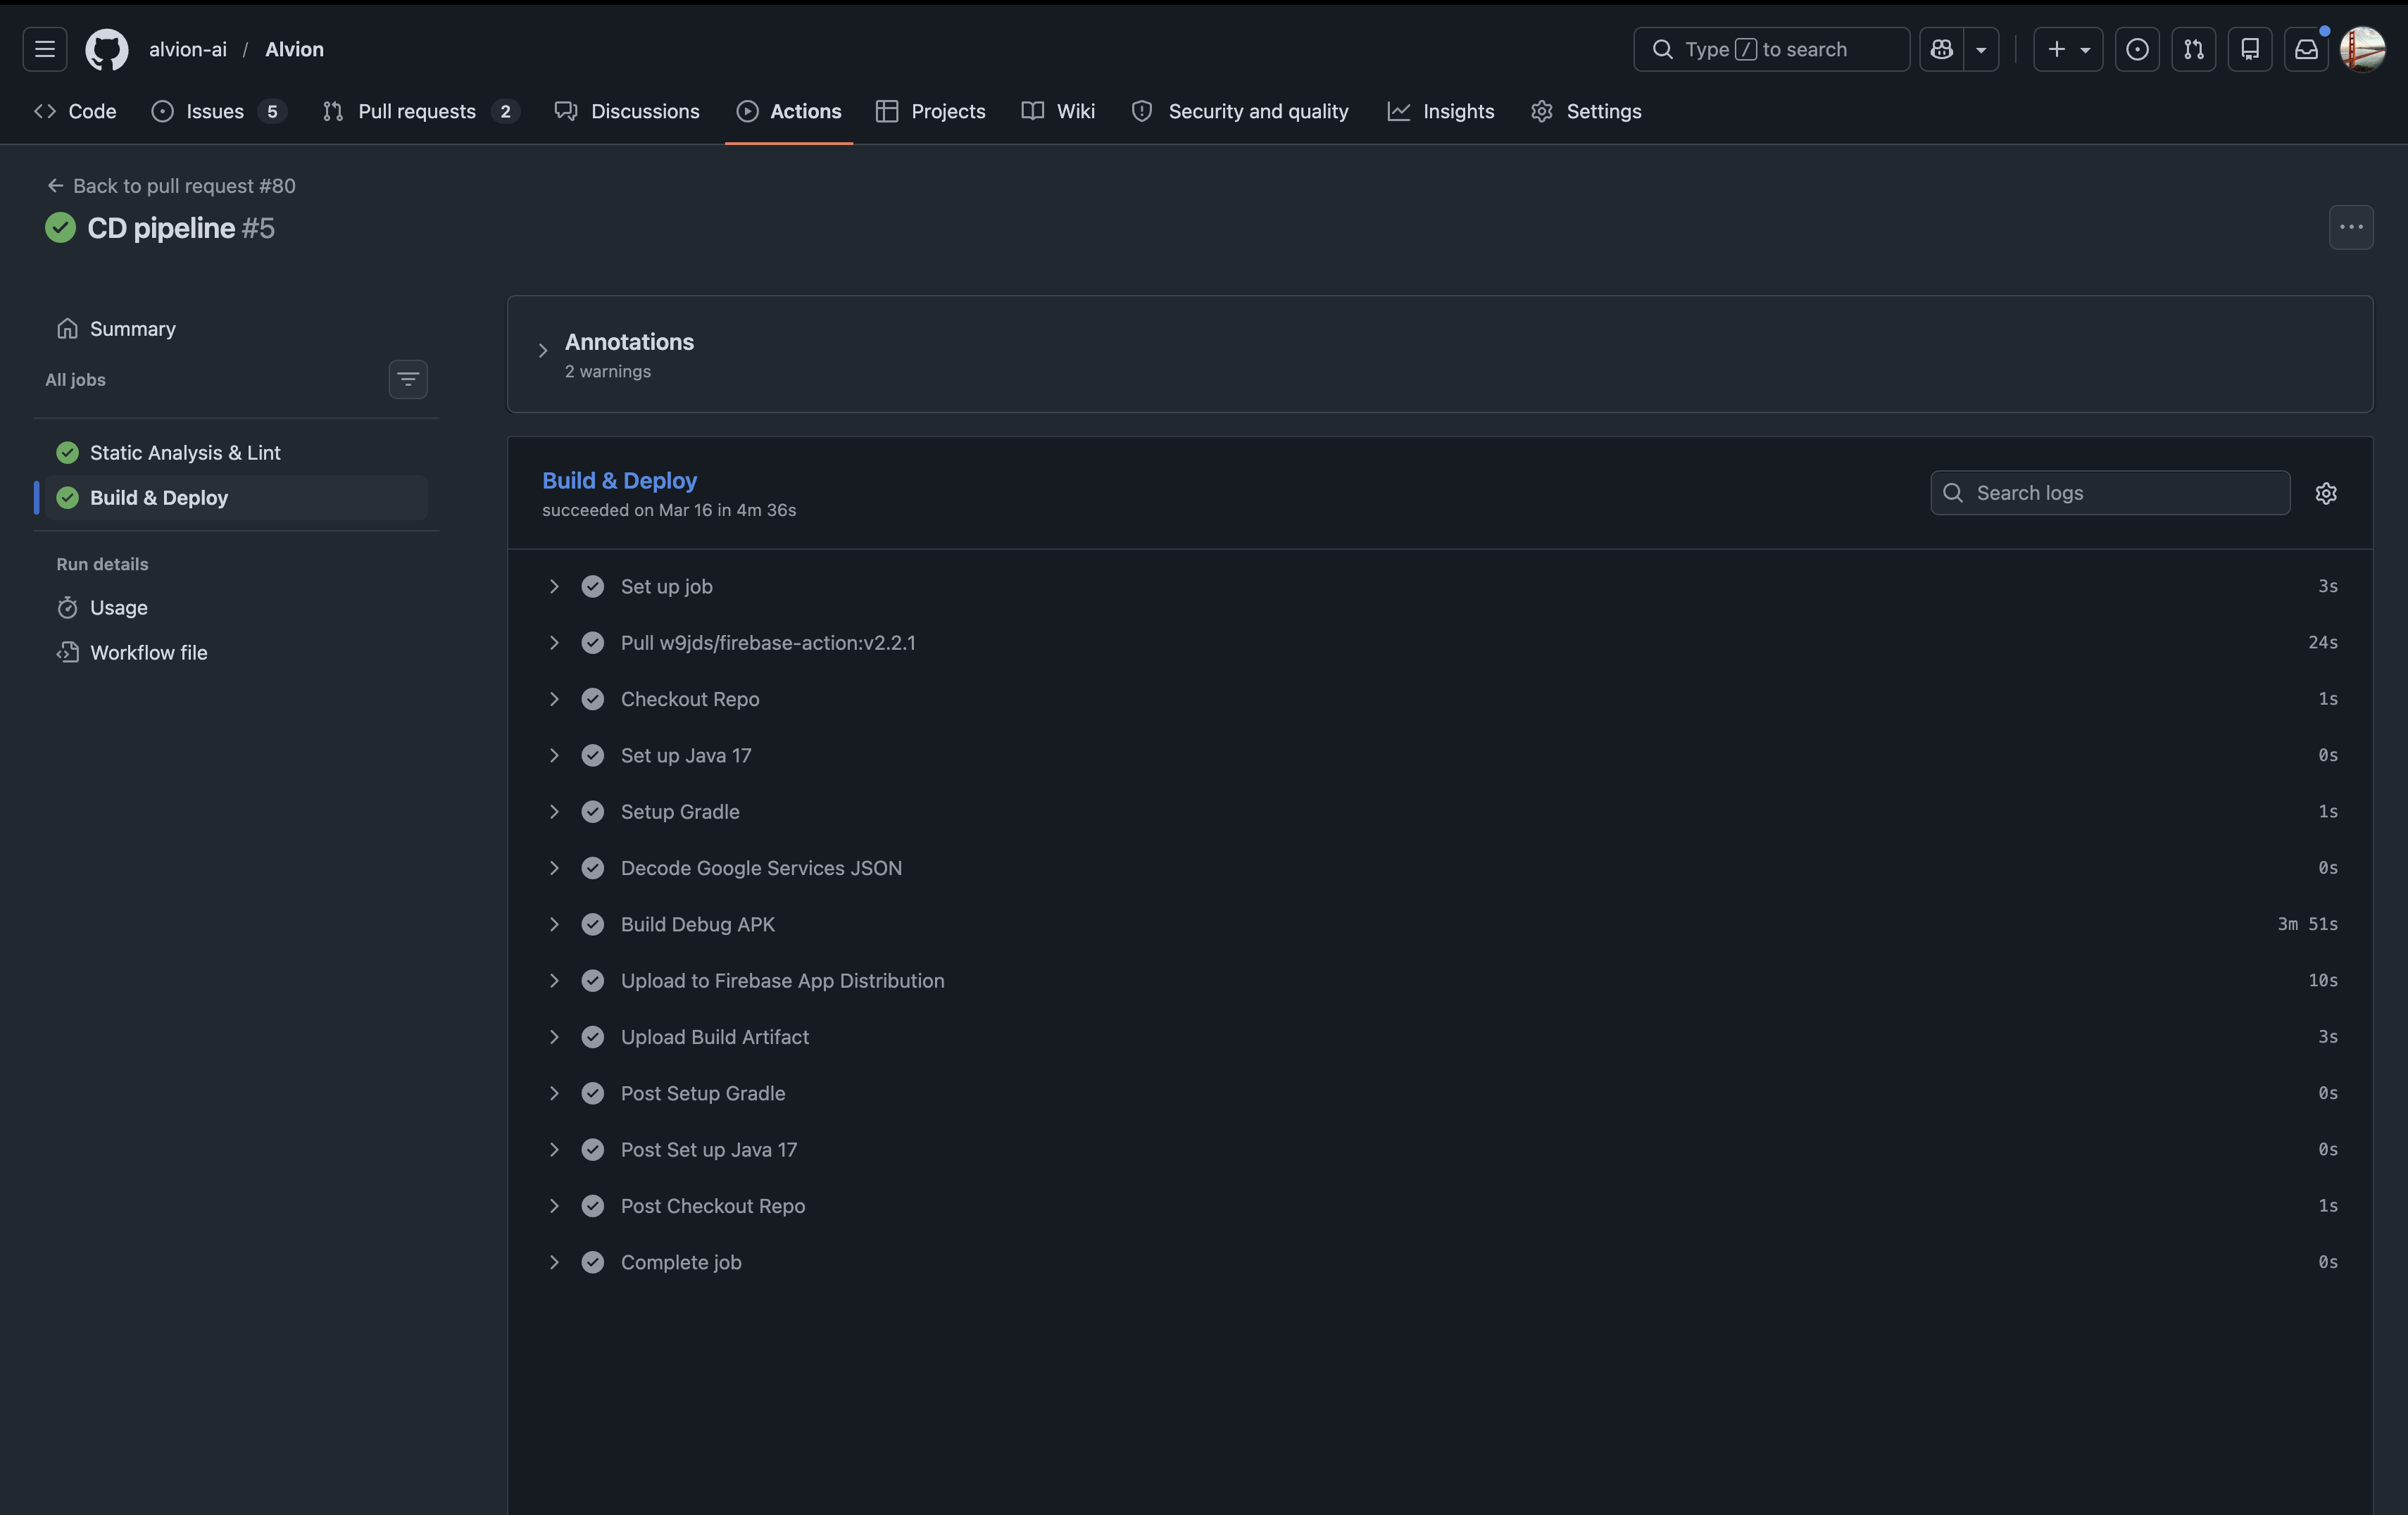
\includegraphics[width=0.98\textwidth]{assets/pm_actions_workflow_runs.png}
    \caption{Successful GitHub Actions workflow run showing automated verification steps such as build, lint, test, or deployment checks.}
    \label{fig:pm-actions-successful-run}
\end{figure}

Figure~\ref{fig:pm-actions-successful-run} shows a detailed successful workflow run. The run demonstrates that the team used automated verification steps as part of the development process. These checks helped reduce the risk of merging broken code and provided repeatable evidence that project changes were validated.

Overall, the CI/CD evidence shows that the team managed quality control through automated workflows. Combined with issue tracking and pull request review, GitHub Actions helped the team maintain a structured process for testing, building, and deploying the ALVION application.

\subsection*{PM.7 Project Management Summary}

The evidence in Appendix PM shows that the ALVION team followed a structured project management process throughout the capstone project. GitHub Issues were used to create and track tasks, classify work using labels, document bugs, manage feature requests, and record remaining open items. This provided a visible record of project progress across documentation, implementation, testing, refactoring, and deployment work.

The pull request records show that the team used a branch-based workflow instead of making direct untracked changes to the main branch. Pull requests documented the purpose of each change, the type of work completed, testing performed, checklist items, commits, changed files, and merge status. This supported review, accountability, and traceability across major project changes.

The contribution records show that work was divided across team members. Individual contributors owned different areas of the project, including UI/UX development, authentication, facial detection, calibration logic, profile and history features, documentation, testing, CI/CD, GPS speed tracking, and audio alert fixes. This demonstrates both task allocation and individual contribution tracking.

The CI/CD records show that the team used automated workflows to support quality control. GitHub Actions helped verify changes through automated checks such as build, lint, testing, and deployment-related steps. This reduced the risk of merging broken changes and provided repeatable evidence that the project was actively maintained.

Overall, the project management evidence demonstrates that the team planned, assigned, reviewed, tested, and completed work across the full project lifecycle. The records included in this appendix support the highest rubric level because they provide detailed project management evidence from GitHub Issues, Pull Requests, contribution records, workflow documentation, CI/CD checks, and remaining open-task tracking.
\end{document}
